% Options for packages loaded elsewhere
\PassOptionsToPackage{unicode}{hyperref}
\PassOptionsToPackage{hyphens}{url}
%
\documentclass[
]{book}
\usepackage{amsmath,amssymb}
\usepackage{lmodern}
\usepackage{iftex}
\ifPDFTeX
  \usepackage[T1]{fontenc}
  \usepackage[utf8]{inputenc}
  \usepackage{textcomp} % provide euro and other symbols
\else % if luatex or xetex
  \usepackage{unicode-math}
  \defaultfontfeatures{Scale=MatchLowercase}
  \defaultfontfeatures[\rmfamily]{Ligatures=TeX,Scale=1}
\fi
% Use upquote if available, for straight quotes in verbatim environments
\IfFileExists{upquote.sty}{\usepackage{upquote}}{}
\IfFileExists{microtype.sty}{% use microtype if available
  \usepackage[]{microtype}
  \UseMicrotypeSet[protrusion]{basicmath} % disable protrusion for tt fonts
}{}
\makeatletter
\@ifundefined{KOMAClassName}{% if non-KOMA class
  \IfFileExists{parskip.sty}{%
    \usepackage{parskip}
  }{% else
    \setlength{\parindent}{0pt}
    \setlength{\parskip}{6pt plus 2pt minus 1pt}}
}{% if KOMA class
  \KOMAoptions{parskip=half}}
\makeatother
\usepackage{xcolor}
\usepackage{color}
\usepackage{fancyvrb}
\newcommand{\VerbBar}{|}
\newcommand{\VERB}{\Verb[commandchars=\\\{\}]}
\DefineVerbatimEnvironment{Highlighting}{Verbatim}{commandchars=\\\{\}}
% Add ',fontsize=\small' for more characters per line
\usepackage{framed}
\definecolor{shadecolor}{RGB}{248,248,248}
\newenvironment{Shaded}{\begin{snugshade}}{\end{snugshade}}
\newcommand{\AlertTok}[1]{\textcolor[rgb]{0.94,0.16,0.16}{#1}}
\newcommand{\AnnotationTok}[1]{\textcolor[rgb]{0.56,0.35,0.01}{\textbf{\textit{#1}}}}
\newcommand{\AttributeTok}[1]{\textcolor[rgb]{0.77,0.63,0.00}{#1}}
\newcommand{\BaseNTok}[1]{\textcolor[rgb]{0.00,0.00,0.81}{#1}}
\newcommand{\BuiltInTok}[1]{#1}
\newcommand{\CharTok}[1]{\textcolor[rgb]{0.31,0.60,0.02}{#1}}
\newcommand{\CommentTok}[1]{\textcolor[rgb]{0.56,0.35,0.01}{\textit{#1}}}
\newcommand{\CommentVarTok}[1]{\textcolor[rgb]{0.56,0.35,0.01}{\textbf{\textit{#1}}}}
\newcommand{\ConstantTok}[1]{\textcolor[rgb]{0.00,0.00,0.00}{#1}}
\newcommand{\ControlFlowTok}[1]{\textcolor[rgb]{0.13,0.29,0.53}{\textbf{#1}}}
\newcommand{\DataTypeTok}[1]{\textcolor[rgb]{0.13,0.29,0.53}{#1}}
\newcommand{\DecValTok}[1]{\textcolor[rgb]{0.00,0.00,0.81}{#1}}
\newcommand{\DocumentationTok}[1]{\textcolor[rgb]{0.56,0.35,0.01}{\textbf{\textit{#1}}}}
\newcommand{\ErrorTok}[1]{\textcolor[rgb]{0.64,0.00,0.00}{\textbf{#1}}}
\newcommand{\ExtensionTok}[1]{#1}
\newcommand{\FloatTok}[1]{\textcolor[rgb]{0.00,0.00,0.81}{#1}}
\newcommand{\FunctionTok}[1]{\textcolor[rgb]{0.00,0.00,0.00}{#1}}
\newcommand{\ImportTok}[1]{#1}
\newcommand{\InformationTok}[1]{\textcolor[rgb]{0.56,0.35,0.01}{\textbf{\textit{#1}}}}
\newcommand{\KeywordTok}[1]{\textcolor[rgb]{0.13,0.29,0.53}{\textbf{#1}}}
\newcommand{\NormalTok}[1]{#1}
\newcommand{\OperatorTok}[1]{\textcolor[rgb]{0.81,0.36,0.00}{\textbf{#1}}}
\newcommand{\OtherTok}[1]{\textcolor[rgb]{0.56,0.35,0.01}{#1}}
\newcommand{\PreprocessorTok}[1]{\textcolor[rgb]{0.56,0.35,0.01}{\textit{#1}}}
\newcommand{\RegionMarkerTok}[1]{#1}
\newcommand{\SpecialCharTok}[1]{\textcolor[rgb]{0.00,0.00,0.00}{#1}}
\newcommand{\SpecialStringTok}[1]{\textcolor[rgb]{0.31,0.60,0.02}{#1}}
\newcommand{\StringTok}[1]{\textcolor[rgb]{0.31,0.60,0.02}{#1}}
\newcommand{\VariableTok}[1]{\textcolor[rgb]{0.00,0.00,0.00}{#1}}
\newcommand{\VerbatimStringTok}[1]{\textcolor[rgb]{0.31,0.60,0.02}{#1}}
\newcommand{\WarningTok}[1]{\textcolor[rgb]{0.56,0.35,0.01}{\textbf{\textit{#1}}}}
\usepackage{longtable,booktabs,array}
\usepackage{calc} % for calculating minipage widths
% Correct order of tables after \paragraph or \subparagraph
\usepackage{etoolbox}
\makeatletter
\patchcmd\longtable{\par}{\if@noskipsec\mbox{}\fi\par}{}{}
\makeatother
% Allow footnotes in longtable head/foot
\IfFileExists{footnotehyper.sty}{\usepackage{footnotehyper}}{\usepackage{footnote}}
\makesavenoteenv{longtable}
\usepackage{graphicx}
\makeatletter
\def\maxwidth{\ifdim\Gin@nat@width>\linewidth\linewidth\else\Gin@nat@width\fi}
\def\maxheight{\ifdim\Gin@nat@height>\textheight\textheight\else\Gin@nat@height\fi}
\makeatother
% Scale images if necessary, so that they will not overflow the page
% margins by default, and it is still possible to overwrite the defaults
% using explicit options in \includegraphics[width, height, ...]{}
\setkeys{Gin}{width=\maxwidth,height=\maxheight,keepaspectratio}
% Set default figure placement to htbp
\makeatletter
\def\fps@figure{htbp}
\makeatother
\setlength{\emergencystretch}{3em} % prevent overfull lines
\providecommand{\tightlist}{%
  \setlength{\itemsep}{0pt}\setlength{\parskip}{0pt}}
\setcounter{secnumdepth}{5}
\usepackage{booktabs}
\usepackage{amsthm}
\usepackage{listings}
\lstset{
  breaklines=true
}
\makeatletter
\def\thm@space@setup{%
  \thm@preskip=8pt plus 2pt minus 4pt
  \thm@postskip=\thm@preskip
}
\makeatother

\usepackage{fvextra}
\usepackage{listings}
\lstset{
breaklines=true
  }
\DefineVerbatimEnvironment{Highlighting}{Verbatim}{
  breaksymbolleft={}, 
  showspaces = false,
  showtabs = false,
  breaklines,
  commandchars=\\\{\}
}

\ifLuaTeX
  \usepackage{selnolig}  % disable illegal ligatures
\fi
\usepackage[]{natbib}
\bibliographystyle{apalike}
\IfFileExists{bookmark.sty}{\usepackage{bookmark}}{\usepackage{hyperref}}
\IfFileExists{xurl.sty}{\usepackage{xurl}}{} % add URL line breaks if available
\urlstyle{same} % disable monospaced font for URLs
\hypersetup{
  pdftitle={Introduction à R et aux statistiques en sciences sociales},
  pdfauthor={Lev Lhommeau},
  hidelinks,
  pdfcreator={LaTeX via pandoc}}

\title{Introduction à R et aux statistiques en sciences sociales}
\author{Lev Lhommeau}
\date{2023-02-16}

\begin{document}
\maketitle

{
\setcounter{tocdepth}{1}
\tableofcontents
}
\hypertarget{remarques-pruxe9liminaires}{%
\chapter{Remarques préliminaires}\label{remarques-pruxe9liminaires}}

Ceci est une introduction au langage de programmation R et à l'analyse statistique en sciences sociales. Ce syllabus s'adresse aux étudiants en sciences sociales, telles que la science politique, la sociologie et la communication, ainsi qu'à toute personne qui souhaite découvrir les bases de l'analyse statistique des phénomènes sociaux avec R. Ce syllabus veut contribuer à combler une lacune dans les publications existantes en langue française: il existe certes de très bons ouvrages théoriques d'introduction aux statistiques à l'usage des sciences sociales, tout comme il existe de bons ouvrages d'introduction à la programmation avec R. En revanche, une introduction pratique à l'analyse des phénomènes sociaux avec R fait encore défaut. C'est cette lacune que vise la présente introduction.

Ce syllabus se fonde sur les travaux pratiques que j'assure sous la direction de Philippe Bocquier et Bruno Schoumaker à l'UCLouvain. Au vu du public cible, les concepts mathématiques et statistiques mobilisés dans cette introduction sont tout à fait abordables. Cette introduction essayera de faire au maximum l'économie de formules mathématiques et si elles sont indispensables, elles s'efforcera de les ``traduire'' en langue française. Il est cependant préférable, si le lecteur ne dispose pas de connaissances en statistiques, d'accompagner la lecture de ce syllabus de la lecture d'un manuel de statistiques ou du suivi d'un cours de statistiques. À cette fin, l'on peut conseiller en langue française, les ressources et ouvrages suivants (liste non exhaustive):

Masuy-Stroobant \& Costa (2013): Analyser les données en sciences sociales. De la préparation des données à l'analyse multivariée, Bruxelles: P.I.E. Peter Lang.

Cette introduction a vocation à être accessible à des personnes sans aucune expérience en programmation. Aucun prérequis en programmation n'est donc requis pour la suivre. Elle ne prétend pas à l'exhaustivité, mais souhaite donner un premier aperçu des statistiques en sciences sociales et des possibilités qu'offre le langage de programmation R. Vu qu'il s'agit d'une introduction aux statistiques, les autres usages de R, notamment pour les présentations (avec \href{https://rmarkdown.rstudio.com/}{\emph{R Markdown}} ou \href{https://shiny.rstudio.com/}{\emph{Shiny}}) et l'automatisation de certaines tâches, ne seront pas traités. Si vous cherchez une introduction spécifique à la programmation en R en langue française, nous vous conseillons, l'ouvrage suivant:

Vincent Goulet: Introduction à la programmation en R, (téléchargez le \href{https://cran.r-project.org/doc/contrib/Goulet_introduction_programmation_R.pdf}{ici})

Notons enfin, que nous avons fait le choix de montrer, outre le R de base, les méthodes issues du \protect\hyperlink{packages}{\emph{package}} \href{https://www.tidyverse.org/}{\emph{tydiverse}}. \href{https://www.tidyverse.org/}{\emph{Tydiverse}} est ce qu'on appelle un ``dialecte'' dans une langue de programmation. Un ``dialecte'' modifie une langue de programmation sans l'altérer fondamentalement. Pourquoi ajouter un ``dialecte'' à cette introduction? Le R de base ne suffit-il pas? Le \href{https://www.tidyverse.org/}{\emph{tydiverse}} est très utilisé et il est donc plus qu'utile de le connaître si l'on souhaite se lancer dans R. De plus, le \href{https://www.tidyverse.org/}{\emph{tydiverse}} avec ses \protect\hyperlink{packages}{\emph{package}} tels que \href{https://dplyr.tidyverse.org/}{\emph{dplyr}} et \href{https://ggplot2.tidyverse.org/}{\emph{ggplot2}} a grandement simplifié la manipulation des données et la réalisation de graphiques de qualité\footnote{Si vous voulez lire une introduction en français plus complète au \emph{tidyverse} nous renvoyons à l'ouvrage \href{https://juba.github.io/tidyverse/}{``Introduction à R et au tidyverse''} de Julien Barnier.}.

\hypertarget{installer-r}{%
\section{Installer R}\label{installer-r}}

Pour suivre cette introduction, veuillez installer le langage de programmation R et \emph{ensuite} l'environnement de développement \href{https://posit.co/}{\emph{RStudio}}\footnote{\href{https://posit.co/}{\emph{RStudio}} est un environnement de développement spécialisé pour R, mais il peut également exécuter le langage de programmation plus généraliste \href{https://www.python.org/}{\emph{Python}}. Vous pouvez également utiliser R sans environnement de développement ou avec un autre environnement que \href{https://posit.co/}{\emph{RStudio}}, tel que \href{https://code.visualstudio.com/}{\emph{VSCode}}. \href{https://posit.co/}{\emph{RStudio}} est cependant l'environnement le plus utilisé pour coder en R et certainement le plus adapté aux débutants.} (bien dans cet ordre-là: installez \textbf{d'abord} R et ensuite \emph{RStudio Desktop}) sur votre ordinateur. R est une langue de programmation libre, c'est-à-dire qu'elle est entièrement gratuite! Plus besoin d'acheter d'onéreuses licences pour des programmes d'analyse statistique payants tels que \href{https://www.stata.com/}{\emph{Stata}}, \href{https://www.ibm.com/fr-fr/products/spss-statistics}{\emph{SPSS}} et \href{https://www.sas.com/}{\emph{SAS}}, bien souvent moins performants que R. \href{https://posit.co/}{\emph{RStudio}} est également gratuit dans sa version de base (\emph{RStudio Desktop}), entièrement suffisante pour l'usage que nous allons en faire.

Pour télécharger R, rendez-vous sur le site du \href{https://cran.r-project.org/}{\emph{CRAN}} et installez la dernière version de R pour votre système d'exploitation (Linux, Windows ou macOS):

\url{https://cran.r-project.org/}

Pour télécharger RStudio rendez-vous sur le site de \emph{posit}, l'entreprise qui développe \href{https://posit.co/}{\emph{RStudio}}, et installez la dernière version de \href{https://posit.co/}{\emph{RStudio}} pour votre système d'exploitation (Linux, Windows ou macOS):

\url{https://posit.co/}

\hypertarget{se-retrouver-uxe0-lintuxe9rieur-de-ce-syllabus}{%
\section{Se retrouver à l'intérieur de ce syllabus}\label{se-retrouver-uxe0-lintuxe9rieur-de-ce-syllabus}}

Ce syllabus est composé de plusieurs chapitres qui abordent chacun des questions différentes. Le syllabus suit une progression: la complexité augmente avec les chapitres. Il est donc conseillé, surtout au début, de bien suivre l'ordre de celui-ci. Au fur et à mesure que vous avancerez, vous pourrez prendre davantage de libertés avec l'ordre dans lequel vous lisez les chapitres.

Vous pouvez naviguer entre les chapitres et les sous-chapitres dans le volet de gauche. Vous pouvez, par ailleurs, naviguer entre les chapitres en appuyant sur les touches de gauche et de droite. Vous pouvez télécharger la version PDF et epub de ce syllabus en cliquant sur l'icône de téléchargement en haut de la page\footnote{Notez que pas toutes les fonctions ``interactives'' de ce syllabus ne pourront pas être maintenus au format PDF et epub et que des difficultés de mise en page ne sont pas exclues.}.

Les codes R à introduire se trouvent dans des encadrés comme celui-ci:

\begin{Shaded}
\begin{Highlighting}[]
\CommentTok{\# Le signe \# marque un commentaire qui sera ignoré par R.}
\CommentTok{\#Si vous voulez afficher le fameux "Hello World", vous pouvez le faire ainsi:}
\FunctionTok{print}\NormalTok{(}\StringTok{"Hello world!"}\NormalTok{)}
\CommentTok{\#Ou ainsi:}
\FunctionTok{message}\NormalTok{(}\StringTok{"Hello world!"}\NormalTok{)}
\end{Highlighting}
\end{Shaded}

Si vous passez votre souris sur cet encadré, vous verrez apparaître, en haut à droite de l'encadré, une icône vous permettant de copier son contenu. Celui-ci pourra être collé dans votre code R puis exécuté. Si vous copiez ce code dans votre R Code puis l'exécutez (ou le copiez directement dans votre console puis appuyez sur la touche ``\emph{Entrée}'' de votre clavier), voilà ce qui devrait apparaître dans votre console:

\begin{verbatim}
## [1] "Hello world!"
\end{verbatim}

\begin{verbatim}
## Hello world!
\end{verbatim}

Si vous avez des questions ou des remarques, n'hésitez pas à me contacter: \href{mailto:lev.lhommeau@uclouvain.be}{\nolinkurl{lev.lhommeau@uclouvain.be}} / \href{mailto:lhommeau@gmail.com}{\nolinkurl{lhommeau@gmail.com}}\footnote{Si je ne réponds pas à l'une de ces adresses, essayez de me contacter par l'autre.}.

\hypertarget{Priseenmain}{%
\chapter{Prise en main de R}\label{Priseenmain}}

\hypertarget{Commandes}{%
\section{Commandes dans R}\label{Commandes}}

Vous vous demandez peut-être comment exécuter des commandes dans R. Si vous utilisez \href{https://posit.co/}{\emph{RStudio}}, vous avez deux possibilités. Vous pouvez indiquer le code directement dans la console qui se trouve dans l'onglet ``Console''. une fois que la commande est introduite, appuyez sur la touche \emph{Entrée} de votre clavier pour la soumettre à l'\href{https://fr.wikipedia.org/wiki/Interpr\%C3\%A8te_(informatique)}{interpréteur} de R. Cependant, cette manière ne sera pas votre moyen principal de soumettre des commandes à R. Vous allez plutôt utiliser des fichiers \emph{R Script} dans lesquels vous noterez votre code: pour créer un nouveau fichier \emph{R Script}, cliquez en haut à gauche dans \href{https://posit.co/}{\emph{RStudio}} sur l'icône représentant une feuille blanche avec un signe plus (+) sur fond vert et choisissez \emph{R Script} dans le menu déroulant.

Un fichier \emph{R Script} est un document texte rassemblant l'ensemble des commandes que vous souhaitez soumettre à R. C'est un peu comme une ``recette'' où chaque commande correspond à un ingrédient ou une manipulation à faire pour obtenir le plat désiré. Sauf, bien entendu, que le plat désiré ne sera pas une mousse au chocolat ou un rôti de bœuf, mais le résultat d'un calcul, d'une manipulation de données, d'une analyse statistique ou une représentation graphique. Ce fichier \emph{R Script} peut être enregistré sous un nom de votre choix suivi du suffixe ``.R'' (par exemple: ``Analyse.R''). Cela vous permet de commenter et de reproduire les commandes que vous avez faites: si vous indiquiez vos commandes uniquement dans la console, vous pourriez que difficilement reproduire vos manipulations et analyses. Or, la reproductibilité est un critère essentiel de la scientificité. Par ailleurs, le code que vous avez écrit peut être réutilisé lors d'analyses futures. Cela vous fera gagner du temps!

Mais comment exécuter les commandes que vous avez notées dans votre fichier de \emph{R Script}? Il suffit de placer le curseur sur une commande et d'appuyer sur la flèche verte ``Run'' qui se situe au-dessus à droite de l'onglet où se trouve votre code. Vous pouvez aussi appuyer sur les touches ``\emph{Contrôle + Entrée}'' de votre clavier. Par ailleurs, vous pouvez sélectionner une partie de votre code, puis exécuter cette partie du code de la même manière.

\hypertarget{Fonctions_aides}{%
\section{Fonctions et aide dans R}\label{Fonctions_aides}}

Comme \href{https://www.microsoft.com/fr-be/microsoft-365/excel}{\emph{Excel}} (ou d'autres langues de programmation tels que \href{https://www.python.org/}{\emph{Python}} ou \emph{C}), R dispose de fonctions que vous allez pouvoir utiliser pour mener vos analyses statistiques et manipuler vos données. En informatique, une fonction est un programme qui exécute une (suite de) commande(s) dont elle retourne un résultat et que l'on peut réutiliser dans d'autres programmes. Les fonctions en R sont composées de leur nom\footnote{Attention: R est sensible à la casse: ``Mean'' est différent de ``mean''. Soyeuz fonc toujours très attentif à la casse lorsque vous codez en R.}, suivi d'une parenthèse dans laquelle vous pourrez indiquer, le cas échéant, les arguments séparés par des virgules. Ainsi, si vous voulez connaitre la moyenne de la suite \(A=\{0,1,2,3,4,5,6,7,8,9,10\}\), vous pouvez utiliser la fonction \href{https://www.rdocumentation.org/packages/base/versions/3.6.2/topics/mean}{\emph{mean()}}. Avant il faut créer le \emph{vecteur}\footnote{Pour savoir comment créer des vecteurs en R, nous renvoyons à la page suivante: \url{http://www.sthda.com/french/wiki/les-vecteurs-vector}.} \emph{suite\_a}:

\begin{Shaded}
\begin{Highlighting}[]
\CommentTok{\#Nous créons la suite A allant de 0 à 10 et la nommons suite\_a dans R:}
\NormalTok{suite\_a}\OtherTok{\textless{}{-}}\FunctionTok{c}\NormalTok{(}\DecValTok{0}\NormalTok{,}\DecValTok{1}\NormalTok{,}\DecValTok{2}\NormalTok{,}\DecValTok{3}\NormalTok{,}\DecValTok{4}\NormalTok{,}\DecValTok{5}\NormalTok{,}\DecValTok{6}\NormalTok{,}\DecValTok{7}\NormalTok{,}\DecValTok{8}\NormalTok{,}\DecValTok{9}\NormalTok{,}\DecValTok{10}\NormalTok{)}

\CommentTok{\#À l\textquotesingle{}aide de la fonction mean(), nous calculons la moyenne de cette suite:}
\FunctionTok{mean}\NormalTok{(suite\_a)}
\end{Highlighting}
\end{Shaded}

\begin{verbatim}
## [1] 5
\end{verbatim}

L'\protect\hyperlink{objets_envir}{objet} suite\_a contenant la suite \(A\) est l'argument de la fonction \href{https://www.rdocumentation.org/packages/base/versions/3.6.2/topics/mean}{\emph{mean()}} que l'on note dans la parenthèse de la fonction. Comme vous pouvez le voir, la moyenne de cette suite \(A\) est de 5.

Si vous avez besoin d'aide concernant une fonction dans R, écrivez la fonction précédée de ``?''. Par exemple:

\begin{Shaded}
\begin{Highlighting}[]
\NormalTok{?setwd}
\end{Highlighting}
\end{Shaded}

Dans RStudio, dans l'onglet ``\emph{Help}'' en bas à droite, s'affiche alors l'aide. Vous pouvez également sélectionner une fonction et appuyer sur la touche ``\emph{F1}'' de votre clavier.

Outre les fonctions déjà existantes dans R et ses \protect\hyperlink{packages}{\emph{packages}}, vous pouvez définir vos propres fonctions. Celles-ci vous permettent de réaliser ce dont vous avez besoin sur mesure (analyse statistique, transformation de données, etc.). Cela peut être réalisé de manière assez simple dans R\footnote{Ce syllabus contient des exemples de fonctions créés, cependant cela ne fait pas partie de ses objets principaux. Nous renvoyons donc à d'autres ouvrages à ce sujet.}.

\hypertarget{working_directory}{%
\section{\texorpdfstring{Espace de travail (\emph{working directory})}{Espace de travail (working directory)}}\label{working_directory}}

Lorsque l'on travaille avec R, il faut définir un espace de travail. C'est le dossier où R sauvegardera et charge les fichiers et bases de données avec lesquels vous travaillez. Si vous ne le déterminez pas, R choisit un dossier par défaut. Sur un ordinateur Windows, cela sera bien souvent le dossier ``Documents''. Nous vous conseillons de créer un dossier dédié à votre travail en R et de définir celui-ci comme répertoire de travail. Si vous aviez créé un dossier ``Espace\_R'' dans un dossier ``Revisions'' sur votre disque dur C, vous soumettriez le code suivant à R pour en faire votre espace de travail:

\begin{Shaded}
\begin{Highlighting}[]
\FunctionTok{setwd}\NormalTok{(}\StringTok{"C:/Revisions/Espace\_R"}\NormalTok{) }\CommentTok{\# Indiquez le chemin du dossier qui doit être votre répertoire de travail}
\end{Highlighting}
\end{Shaded}

Vous aurez remarqué que le chemin d'accès et les dossiers sont entre guillemets. Par ailleurs, dans R, les chemins d'accès entre dossiers (``Revision'') et sous-dossiers (``Espace\_R'') sont séparés par des barres obliques (/), comme pour une division. Dans Windows, les chemins d'accès sont notés par des barres obliques inversées (\textbackslash). Il faut donc corriger cela lorsque vous copiez des chemins d'accès dans R.

Sous Windows, vous pouvez aussi choisir manuellement le dossier dans lequel se trouve votre espace de travail:

\begin{Shaded}
\begin{Highlighting}[]
\FunctionTok{setwd}\NormalTok{(}\FunctionTok{choose.dir}\NormalTok{()) }\CommentTok{\# Indiquez le chemin du dossier qui doit être votre répertoire de travail}
\end{Highlighting}
\end{Shaded}

Si vous lancez ce code, une fenêtre s'ouvre dans laquelle vous pourrez cliquer sur le dossier que vous souhaitez déterminer en tant que dossier de travail. Malheureusement, cela fonctionne uniquement sous Windows et pas sous Linux et macOS.

Que votre système d'exploitation soit Linux, macOS ou Windows, vous pouvez définir votre espace de travail grâce aux menus de \href{https://posit.co/}{\emph{RStudio}}. Allez sur le menu ``Session'' puis choisissez ``\emph{Set Working Directory}'' dans le menu déroulant. Parmi les options disponibles cliquez sur ``\emph{Choose Directory}''. Une fenêtre s'ouvre alors dans laquelle vous pourrez choisir le fichier de votre choix pour déterminer l'emplacement de votre espace de travail.

\hypertarget{packages}{%
\section{\texorpdfstring{Installer et lancer des \emph{packages} (bibliothèques)}{Installer et lancer des packages (bibliothèques)}}\label{packages}}

Comme d'autres langues de programmation, R dispose d'un grand nombre de \emph{packages}\footnote{En français, l'on parle de bibliothèques. Nous alignons cependant ce syllabus sur l'usage en anglais que l'on retrouve dans R. Nous parlerons donc de \emph{package(s)}.}. Ceux-ci enrichissent le langage de nouvelles fonctions qui n'étaient pas encore présentes dans sa version initiale. R est particulièrement riche en \emph{packages.} Sur \href{https://cran.r-project.org/}{\emph{CRAN}}, le répertoire ``officiel'' de R, \(19136\) \emph{packages} étaient répertoriés en janvier 2023.

Pour installer un \emph{package}, il y a la commande générique \emph{install.packages()}. Lors de cette formation, nous allons beaucoup utiliser des \emph{packages} issus du \href{https://www.tidyverse.org/}{\emph{tydiverse}}, un ensemble de \emph{packages}, permettant de manipuler les données et de les représenter graphiquement. Cette suite de \emph{packages} est particulièrement populaire et très largement utilisée. Nous allons donc installer cet ensemble de \emph{packages} avec la commande \href{https://www.rdocumentation.org/packages/utils/versions/3.6.2/topics/install.packages}{\emph{install.packages()}}:

\begin{Shaded}
\begin{Highlighting}[]
\FunctionTok{install.packages}\NormalTok{(tidyverse, }\AttributeTok{dependencies=}\NormalTok{T) }\CommentTok{\#l\textquotesingle{}argument "dependencies=T" permet}
        \CommentTok{\#d\textquotesingle{}installer automatiquement tous les packages dont à besoin le package}
        \CommentTok{\#que l\textquotesingle{}on installe pour fonctionner correctement.}
\end{Highlighting}
\end{Shaded}

Installer un \emph{package} ne suffit pas pour l'utiliser. Il doit être chargé à chaque fois que R est fermé puis redémarré. Cela se fait avec la commande \href{https://www.rdocumentation.org/packages/base/versions/3.6.2/topics/library}{\emph{library()}}. Lançons donc le package \emph{tidyverse}:

\begin{Shaded}
\begin{Highlighting}[]
\FunctionTok{library}\NormalTok{(tidyverse)}
\end{Highlighting}
\end{Shaded}

Le \emph{package} est à présent chargé et peut être utilisé. Si R vous retourne une erreur lorsque vous chargez un \emph{package}, cela est souvent dû au fait que le \emph{package} demandé n'est pas (correctement) installé (vérifiez aussi de l'avoir orthographié correctement et d'avoir respecté la casse). Si vous lancez une fonction et que celle-ci ne s'exécute pas (et renvoie une erreur), vérifiez que le \emph{package} à laquelle elle appartient est bien chargé. Vous verrez cela dans l'onglet ``\emph{Packages}'' en bas à droite de \href{https://posit.co/}{\emph{RStudio}}: si le \emph{package} apparaît dans la liste, c'est qu'il est installé. S'il est coché, c'est qu'il est chargé. S'il n'apparaît pas dans la liste, installez-le. S'il n'est pas coché, lancez-le. Vous pouvez le lancer avec la commande \href{https://www.rdocumentation.org/packages/base/versions/3.6.2/topics/library}{\emph{library()}}, mais vous pouvez aussi la lancer en cochant le \emph{package} dans l'onglet.

Une façon plus simple d'installer et de charger les \emph{packages} est le package \href{http://trinker.github.io/pacman/vignettes/Introduction_to_pacman.html}{\emph{pacman}}. Celui-ci permet d'installer les \emph{packages} et de les lancer en une seule commande: \href{https://www.rdocumentation.org/packages/pacman/versions/0.5.1/topics/p_load}{\emph{p\_load}}. Cette commande vérifie si un \emph{package} est installé: s'il est installé, il le lance, s'il ne l'est pas, il l'installe, puis le lance. Cela peut rendre le lancement de \emph{packages} plus facile et rapide. Par ailleurs, cela permet de plus facilement partager son code: l'interlocuteur peut exécuter votre code sans devoir vérifier s'il a installé les \emph{packages} que vous utilisez:

\begin{Shaded}
\begin{Highlighting}[]
\ControlFlowTok{if}\NormalTok{ (}\SpecialCharTok{!}\FunctionTok{require}\NormalTok{(}\StringTok{"pacman"}\NormalTok{)) }\FunctionTok{install.packages}\NormalTok{(}\StringTok{"pacman"}\NormalTok{) }\CommentTok{\#Cela vérifie}
                             \CommentTok{\#si le package pacman est installé.}
                             \CommentTok{\#S\textquotesingle{}il ne l\textquotesingle{}est pas, il est installé.}

\NormalTok{pacman}\SpecialCharTok{::}\FunctionTok{p\_load}\NormalTok{(tidyverse) }\CommentTok{\#On lance le package tidyverse s\textquotesingle{}il est installé,}
                          \CommentTok{\#sinon on l\textquotesingle{}installe puis le lance automatiquement.}
\end{Highlighting}
\end{Shaded}

Si vous voulez lancer plusieurs \emph{packages} en même temps, il suffit de les ajouter à la suite, séparés par des virgules, entre les parenthèses suivant la fonction \href{https://www.rdocumentation.org/packages/pacman/versions/0.5.1/topics/p_load}{\emph{p\_load}}. Ainsi, si nous voulions charger les \emph{packages} du \href{https://www.tidyverse.org/}{\emph{tydiverse}}, ainsi que le \emph{package} \href{https://rstudio.github.io/DT/}{\emph{DT}}\footnote{Le \emph{package} \emph{DT} permet de créer des tableaux interactifs assez pratiques pour se faire une idée des données. Attention cependant, car les bases de données avec un nombre trop important de lignes (des dizaines de milliers) peuvent faire ``crasher'' R.}.

\begin{Shaded}
\begin{Highlighting}[]
\ControlFlowTok{if}\NormalTok{ (}\SpecialCharTok{!}\FunctionTok{require}\NormalTok{(}\StringTok{"pacman"}\NormalTok{)) }\FunctionTok{install.packages}\NormalTok{(}\StringTok{"pacman"}\NormalTok{) }\CommentTok{\#Cela vérifie}
                             \CommentTok{\#si le package pacman est installé.}
                             \CommentTok{\#S\textquotesingle{}il ne l\textquotesingle{}est pas, il est installé.}

\NormalTok{pacman}\SpecialCharTok{::}\FunctionTok{p\_load}\NormalTok{(tidyverse, DT) }\CommentTok{\#La liste des packages, séparés}
                      \CommentTok{\#par des virgules, que l\textquotesingle{}on souhaite}
                      \CommentTok{\#charger et, si nécessaire, installer.}
\end{Highlighting}
\end{Shaded}

Vous pouvez aligner à la suite autant de \emph{packages} que vous le souhaiter en les séparant par des virgules.

Dans ce syllabus, nous allons utiliser cette méthode avec \href{http://trinker.github.io/pacman/vignettes/Introduction_to_pacman.html}{\emph{pacman}} pour éviter de devoir vérifier si certains \emph{packages} sont installés avant de les lancer.

\hypertarget{objets_envir}{%
\section{Objets et environnement dans R}\label{objets_envir}}

R est une langue de programmation orientée objet. Cela signifie que l'on définit des objets (bases de données, valeurs, fonctions, etc.) que l'on fait interagir les uns avec les autres pour obtenir le résultat escompté\footnote{Une introduction un peu technique à la programmation orientée objet (POO) se trouve ici: \url{https://hdd34.developpez.com/cours/artpoo/}}. Vous pouvez vous imaginer cela un peu comme différentes pièces de ``Légo'' que vous assemblez pour construire un château à votre goût.

Dans R, l'on crée un objet avec le symbole ``\textless-'', une flèche pointant vers la gauche. La flèche montre vers le nom de l'objet à créer à gauche et à droite l'on définit le contenu de cet objet (valeur, vecteur, matrice, etc.).

L'on peut ainsi créer l'objet \emph{bombe\_atomique} qui contient la valeur \(1000^2\):

\begin{Shaded}
\begin{Highlighting}[]
\NormalTok{bombe\_atomique }\OtherTok{\textless{}{-}} \DecValTok{1000}\SpecialCharTok{\^{}}\DecValTok{2} \CommentTok{\# À gauche: le nom de l\textquotesingle{}objet (bombe\_atomique), à droite la valeur}
                         \CommentTok{\#qu\textquotesingle{}elle contient (1000\^{}2)}
\NormalTok{bombe\_atomique           }\CommentTok{\#Maintenant, on se fait afficher le contenu de cet objet dans la console.}
\end{Highlighting}
\end{Shaded}

\begin{verbatim}
## [1] 1e+06
\end{verbatim}

La valeur de l'objet \emph{bombe\_atomique} apparaît dans la console. Par ailleurs, le nom de l'objet apparaît en haut à droite dans l'onglet ``\emph{Environement}'' de \emph{RStudio}. Si vous avez calculé la moyenne de la suite \(A\) dans la section \protect\hyperlink{Fonctions_aides}{Fonctions et aide dans R}, vous y verrez aussi l'objet \emph{suite\_a}. Dans R un environnement\footnote{R connaît plusieurs environnements. L'environnement où est enregistré l'objet définit sa portée, c'est-à-dire dans quelles circonstances les objets sont accessibles. Dans ce syllabus, nous utiliserons consciemment (pratiquement) exclusivement l'environnement global dénommé ``\emph{.GlobalEnv}''. Vu qu'il s'agit d'une introduction, nous ne nous attardons pas sur ce point.} est un espace où les objets sont enregistrés vous permettant de les analyser et de les manipuler.

Vous aurez peut-être remarqué que la valeur de l'objet \emph{bombe\_atomique} est affichée en notation scientifique:

\begin{verbatim}
## [1] 1e+06
\end{verbatim}

Vous pouvez désactiver cet affichage avec la commande suivante:

\begin{Shaded}
\begin{Highlighting}[]
\FunctionTok{options}\NormalTok{(}\AttributeTok{scipen=}\DecValTok{999}\NormalTok{)}
\end{Highlighting}
\end{Shaded}

Vérifiez à nouveau la valeur de l'objet \emph{bombe\_atomique}:

\begin{Shaded}
\begin{Highlighting}[]
\NormalTok{bombe\_atomique}
\end{Highlighting}
\end{Shaded}

\begin{verbatim}
## [1] 1000000
\end{verbatim}

Comme vous pouvez le voir, la notation scientifique à disparue. Cela peut vous faciliter la lecture des résultats de vos analyses!

\hypertarget{import_donnees}{%
\section{Importer et enregistrer des données}\label{import_donnees}}

R dispose de nombreuses fonctions intégrées pour importer des données sous différents formats (\emph{read.table}, \emph{read.delim}, \emph{read.csv}, etc.). Il y a, par ailleurs, un certain nombre de \emph{packages} qui ajoutent de nouvelles fonctions et d'autres formats de données que l'on peut intégrer.

Ainsi, le package \href{https://readr.tidyverse.org/}{\emph{readr}}, appartenant à ``l'univers'' \href{https://www.tidyverse.org/}{\emph{tydiverse}} étant ainsi automatiquement chargé si vous chargez le \href{https://www.tidyverse.org/}{\emph{tydiverse}} (voir \protect\hyperlink{packages}{ici}), ajoute des fonctions assez intéressantes pour charger des données au format texte (\emph{csv}, \emph{txt}): \emph{read\_delim}, \emph{read\_csv}, \emph{read\_csv2}, etc. De même, le \emph{package} \href{https://readxl.tidyverse.org/}{\emph{readxl}} permet de charger des fichiers au format Excel dans R. Bien que ce \emph{package} appartienne également à ``l'univers'' \href{https://www.tidyverse.org/}{\emph{tydiverse}}, le \emph{package} \href{https://readr.tidyverse.org/}{\emph{readr}} doit être chargé séparément. Un troisième \emph{package} issu de cet ``univers'' est le \emph{package} \href{https://haven.tidyverse.org/}{\emph{haven}}: il permet de charger des bases de données enregistrées au format des logiciels statistiques payants \href{https://www.sas.com/}{\emph{SAS}}, \href{https://www.stata.com/}{\emph{Stata}} et \href{https://www.ibm.com/fr-fr/products/spss-statistics}{\emph{SPSS}}. En effet, beaucoup de bases de données sont enregistrées dans l'un de ces formats qui ont l'avantage, contrairement aux formats \emph{CSV} et \emph{Excel}, de pouvoir notamment enregistrer des libellées des variables et des valeurs. Le \emph{package} \href{https://haven.tidyverse.org/}{\emph{haven}} permet de préserver ces avantages lorsque l'on importe les données dans R:

\begin{Shaded}
\begin{Highlighting}[]
\ControlFlowTok{if}\NormalTok{ (}\SpecialCharTok{!}\FunctionTok{require}\NormalTok{(}\StringTok{"pacman"}\NormalTok{)) }\FunctionTok{install.packages}\NormalTok{(}\StringTok{"pacman"}\NormalTok{) }\CommentTok{\#Cela vérifie}
                             \CommentTok{\#si le package pacman est installé.}
                             \CommentTok{\#S\textquotesingle{}il ne l\textquotesingle{}est pas, il est installé.}

\NormalTok{pacman}\SpecialCharTok{::}\FunctionTok{p\_load}\NormalTok{(readxl,haven) }\CommentTok{\#On lance les packages readxl et haven.}
\end{Highlighting}
\end{Shaded}

Lors de cette introduction nous allons utiliser les données issues de l'Enquête sociale européenne/\href{https://www.europeansocialsurvey.org/}{\emph{European social survey (ESS)}}\footnote{Davantage d'informations sur l'Enquête sociale européenne peuvent être trouvées sur son site: \url{https://www.europeansocialsurvey.org/about/}}. Nous allons utiliser la version 9 de l'\href{https://www.europeansocialsurvey.org/}{\emph{ESS}} (ESS 9), contenant des données récoltées en 2018. Les données de l'\href{https://www.europeansocialsurvey.org/}{\emph{ESS}} sont mises à disposition aux formats \href{https://www.ibm.com/fr-fr/products/spss-statistics}{\emph{SPSS}} (avec le suffixe ``.sav''), \href{https://www.stata.com/}{\emph{Stata}} (avec le suffixe ``.dta'') et \href{https://www.sas.com/}{\emph{SAS}} (avec le suffixe ``.sas''). Nous allons télécharger les données de l'\href{https://www.europeansocialsurvey.org/}{\emph{ESS}} au format \href{https://www.ibm.com/fr-fr/products/spss-statistics}{\emph{SPSS}} (avec le suffixe ``.sav'').

Pour pouvoir télécharger les données, il faut s'inscrire sur le site de l'\href{https://www.europeansocialsurvey.org/}{\emph{ESS}}. Cette inscription est entièrement gratuite. Les données de l'\href{https://www.europeansocialsurvey.org/}{\emph{ESS}} peuvent être librement utilisées à des fins non commerciales, notamment pour la recherche et l'enseignement. Nous vous demanderons de vous inscrire sur le le \href{https://www.europeansocialsurvey.org/}{site} de l'\href{https://www.europeansocialsurvey.org/}{\emph{ESS}} et de télécharger les données: téléchargez les données de l'\href{https://www.europeansocialsurvey.org/}{\emph{ESS}} 9 (\emph{ESS Round 9}) pour tous les pays au format \href{https://www.ibm.com/fr-fr/products/spss-statistics}{\emph{SPSS}} (fichier se terminant par ``.sav'').

Nous vous laissons suivre les indications sur le site (en anglais) pour vous inscrire et télécharger les données\footnote{Si vous suivez un enseignement avec \href{mailto:lhommeau@gmail.com}{Lev Lhommeau}, il se peut que ces données vous soient mises à disposition dans ce cadre.}. Il existe le \emph{package} \href{https://cran.r-project.org/web/packages/essurvey/vignettes/intro_ess.html}{\emph{esssurvey}} qui permettait de télécharger directement les données de l'\href{https://www.europeansocialsurvey.org/}{\emph{ESS}} dans R. Malheureusement, en raison de changements concernant l'accès aux données de l'\href{https://www.europeansocialsurvey.org/}{\emph{ESS}} au cours de 2022, ce \emph{package} ne fonctionne plus (janvier 2023).

Une fois que vous avez téléchargé le fichier de l'\href{https://www.europeansocialsurvey.org/}{\emph{ESS}} 9 (2018) au format \href{https://www.ibm.com/fr-fr/products/spss-statistics}{\emph{SPSS}} (fichier se terminant par ``.sav''), il faudra charger la base de données dans R. Pour cela, copiez le fichier dans le dossier dans lequel se trouve votre \protect\hyperlink{working_directory}{espace de travail} R\footnote{Il est possible de charger des fichiers ne se trouvant pas dans votre \protect\hyperlink{working_directory}{espace de travail}. Cela nécessite cependant d'indiquer l'ensemble du chemin d'accès dans R, ce qui peut être laborieux.}. Notre fichier se nomme ``ESS9e03\_1.sav''. Adapter le nom du fichier, s'il porte un autre nom chez vous. Une fois que le fichier de l'\href{https://www.europeansocialsurvey.org/}{\emph{ESS}} 9 se trouve dans votre espace de travail, indiquez le code suivant\footnote{L'exécution de cette commande nécessite le chargement préalable du \emph{package} ``\emph{haven}'', comme indiqué plus haut.}:

\begin{Shaded}
\begin{Highlighting}[]
\NormalTok{ESS9}\OtherTok{\textless{}{-}}\FunctionTok{read\_sav}\NormalTok{(}\StringTok{"ESS9e03\_1.sav"}\NormalTok{) }\CommentTok{\#Vous indiquez le nom de votre fichier}
                      \CommentTok{\#entre guillemets (""). Si le fichier ne se}
                      \CommentTok{\#trouve pas dans votre espace de travail, vous}
                      \CommentTok{\#devrez indiquer tout le chemin d\textquotesingle{}accès.}
\end{Highlighting}
\end{Shaded}

Avec cette commande, vous avez chargé la base de données dans l'environnement de R. Vous l'avez nommé ``ESS9''\footnote{Vous aurez aussi pu la nommer différemment. Pour cela il suffit de changer le nom à gauche de la flèche (\textless-).}. Elle apparaît dans l'onglet ``\emph{Environement}'' en haut à droite de \href{https://posit.co/}{\emph{RStudio}}. Si vous utilisez le système d'exploitation Windows, vous pouvez aussi utiliser la commande \emph{choose.files} à l'intérieur de la fonction \emph{read\_sav}. Lorsque vous exécutez cette commande, une fenêtre s'ouvre vous permettant de choisir manuellement le fichier à charger:

\begin{Shaded}
\begin{Highlighting}[]
\NormalTok{ESS9}\OtherTok{\textless{}{-}}\FunctionTok{read\_sav}\NormalTok{(}\FunctionTok{choose.files}\NormalTok{())}
\end{Highlighting}
\end{Shaded}

Le fichier étant chargé dans l'environnement, vous pouvez l'étudier et le manipuler dans R. Sélectionnez l'objet et exécutez-le:

\begin{Shaded}
\begin{Highlighting}[]
\NormalTok{ESS9}
\end{Highlighting}
\end{Shaded}

Dans votre console s'affichera alors un extrait de la base de données:

\begin{verbatim}
## # A tibble: 49,519 x 572
##    name  essro~1 edition prodd~2  idno cntry    dweight pspwght pweight anwei~3 nwspol netus~4 netustm ppltrst pplfair pplhlp polintr pspps~5 actro~6 psppi~7 cptpp~8 trstprl
##    <chr>   <dbl> <chr>   <chr>   <dbl> <chr+lb>   <dbl>   <dbl>   <dbl>   <dbl> <dbl+> <dbl+l> <dbl+l> <dbl+l> <dbl+l> <dbl+> <dbl+l> <dbl+l> <dbl+l> <dbl+l> <dbl+l> <dbl+l>
##  1 ESS9~       9 3.1     17.02.~    27 AT [Aus~   0.581   0.218   0.302  0.0659 60     5 [Eve~ 180     2 [2]   2 [2]   2 [2]  3 [Har~ 3 [Som~ 2 [A l~ 2 [Ver~ 2 [A l~ 5 [5]  
##  2 ESS9~       9 3.1     17.02.~   137 AT [Aus~   1.06    0.413   0.302  0.125  10     5 [Eve~  20     7 [7]   8 [8]   7 [7]  2 [Qui~ 3 [Som~ 2 [A l~ 3 [Som~ 2 [A l~ 7 [7]  
##  3 ESS9~       9 3.1     17.02.~   194 AT [Aus~   1.38    2.27    0.302  0.686  60     4 [Mos~ 180     5 [5]   7 [7]   7 [7]  4 [Not~ 2 [Ver~ 1 [Not~ 3 [Som~ 2 [A l~ 6 [6]  
##  4 ESS9~       9 3.1     17.02.~   208 AT [Aus~   0.993   0.386   0.302  0.117  45     5 [Eve~ 120     3 [3]   9 [9]   5 [5]  3 [Har~ 2 [Ver~ 2 [A l~ 3 [Som~ 1 [Not~ 0 [No ~
##  5 ESS9~       9 3.1     17.02.~   220 AT [Aus~   0.377   1.03    0.302  0.312  30     1 [Nev~  NA     5 [5]   8 [8]   4 [4]  2 [Qui~ 1 [Not~ 1 [Not~ 1 [Not~ 3 [Qui~ 7 [7]  
##  6 ESS9~       9 3.1     17.02.~   254 AT [Aus~   1.48    0.576   0.302  0.174  45     2 [Onl~  NA     8 [8]   7 [7]   6 [6]  2 [Qui~ 2 [Ver~ 2 [A l~ 3 [Som~ 2 [A l~ 6 [6]  
##  7 ESS9~       9 3.1     17.02.~   290 AT [Aus~   0.992   0.721   0.302  0.218  60     1 [Nev~  NA     6 [6]   1 [1]   3 [3]  4 [Not~ 2 [Ver~ 2 [A l~ 3 [Som~ 2 [A l~ 0 [No ~
##  8 ESS9~       9 3.1     17.02.~   301 AT [Aus~   0.310   0.130   0.302  0.0393 30     1 [Nev~  NA     7 [7]   7 [7]   7 [7]  3 [Har~ 1 [Not~ 1 [Not~ 1 [Not~ 2 [A l~ 5 [5]  
##  9 ESS9~       9 3.1     17.02.~   305 AT [Aus~   1.23    1.77    0.302  0.535  30     5 [Eve~ 120     2 [2]   9 [9]   9 [9]  3 [Har~ 1 [Not~ 1 [Not~ 1 [Not~ 4 [Ver~ 1 [1]  
## 10 ESS9~       9 3.1     17.02.~   400 AT [Aus~   0.459   0.743   0.302  0.224  25     4 [Mos~ 360     7 [7]   4 [4]   4 [4]  4 [Not~ 2 [Ver~ 2 [A l~ 2 [Ver~ 1 [Not~ 3 [3]  
## # ... with 49,509 more rows, 550 more variables: trstlgl <dbl+lbl>, trstplc <dbl+lbl>, trstplt <dbl+lbl>, trstprt <dbl+lbl>, trstep <dbl+lbl>, trstun <dbl+lbl>,
## #   vote <dbl+lbl>, prtvtcat <dbl+lbl>, prtvtdbe <dbl+lbl>, prtvtdbg <dbl+lbl>, prtvtgch <dbl+lbl>, prtvtbcy <dbl+lbl>, prtvtecz <dbl+lbl>, prtvede1 <dbl+lbl>,
## #   prtvede2 <dbl+lbl>, prtvtddk <dbl+lbl>, prtvtgee <dbl+lbl>, prtvtees <dbl+lbl>, prtvtdfi <dbl+lbl>, prtvtdfr <dbl+lbl>, prtvtcgb <dbl+lbl>, prtvtahr <dbl+lbl>,
## #   prtvtfhu <dbl+lbl>, prtvtcie <dbl+lbl>, prtvtcis <dbl+lbl>, prtvtcit <dbl+lbl>, prtvblt1 <dbl+lbl>, prtvblt2 <dbl+lbl>, prtvblt3 <dbl+lbl>, prtvtalv <dbl+lbl>,
## #   prtvtme <dbl+lbl>, prtvtgnl <dbl+lbl>, prtvtbno <dbl+lbl>, prtvtdpl <dbl+lbl>, prtvtcpt <dbl+lbl>, prtvtrs <dbl+lbl>, prtvtcse <dbl+lbl>, prtvtfsi <dbl+lbl>,
## #   prtvtdsk <dbl+lbl>, contplt <dbl+lbl>, wrkprty <dbl+lbl>, wrkorg <dbl+lbl>, badge <dbl+lbl>, sgnptit <dbl+lbl>, pbldmn <dbl+lbl>, bctprd <dbl+lbl>, pstplonl <dbl+lbl>,
## #   clsprty <dbl+lbl>, prtcldat <dbl+lbl>, prtcldbe <dbl+lbl>, prtcldbg <dbl+lbl>, prtclgch <dbl+lbl>, prtclbcy <dbl+lbl>, prtclecz <dbl+lbl>, prtclede <dbl+lbl>, ...
\end{verbatim}

Comme pour d'autres logiciels statistiques, les colonnes représentent les variables et les lignes les observations. Ici, une vingtaine de variables sont affichées (sur \(572\)). De même, les dix premières observations (sur \(49519\)) sont affichées\footnote{Cet affichage est le réglage par défaut d'un \href{https://tibble.tidyverse.org/}{\emph{tibble}}, une forme spéciale de base données dans R. Si vous avez une base de données par défaut (\emph{data.frame}) de R, cela s'affichera un peu différemment. Pour plus de détails en français: \url{https://juba.github.io/tidyverse/06-tidyverse.html}}. Si vous voulez voir l'ensemble de la base de données, vous pouvez utiliser la fonction \emph{View()}\footnote{Mais attention, la base de données étant grande avec près de \(500000\) observations, cela peut prendre un certain temps.}:

\begin{Shaded}
\begin{Highlighting}[]
\FunctionTok{View}\NormalTok{(ESS9)}
\end{Highlighting}
\end{Shaded}

Si vous voulez enregistrer la base de données sous un format R, utilisez le format \emph{RDS}. Celui-ci vous permet d'enregistrer un objet R. La base de données de l'\href{https://www.europeansocialsurvey.org/}{\emph{ESS}} étant chargé sous le nom ``\emph{ESS9}'' comme objet R dans l'\protect\hyperlink{objets_envir}{environnement global} il vous suffira d'exécuter la commande \emph{saveRDS()} pour l'enregistrer. Dans cette commande vous indiquez le nom de l'objet R à enregistrer en tant que premier argument. Ensuite, vous indiquez, séparé par une virgule, comme second argument, le nom sous lequel vous voulez enregistrer l'objet. Ce nom doit être indiqué entre guillemets. Ici, nous voulons enregistrer l'objet ``\emph{ESS9}'' sous le nom ``ESS9.RDS'', afin de le réutiliser lors du prochain chapitre. Exécutez donc le code suivant:

\begin{Shaded}
\begin{Highlighting}[]
\FunctionTok{saveRDS}\NormalTok{(ESS9,}\StringTok{"ESS9.RDS"}\NormalTok{)}
\end{Highlighting}
\end{Shaded}

Le fichier ``ESS9.RDS'' contenant votre base de données est alors enregistré dans votre \protect\hyperlink{working_directory}{espace de travail}. Vous pourrez la charger ensuite pour continuer à travailler avec. C'est ce que nous allons faire dans le prochain chapitre portant sur les distributions.

\hypertarget{close_R}{%
\section{Fermer R}\label{close_R}}

Lorsque vous fermez R, \href{https://posit.co/}{\emph{RStudio}} va vous proposer d'enregistrer l'\protect\hyperlink{objets_envir}{environnement global}. Si vous l'acceptez, un fichier contenant tous les objets se trouvant dans votre \protect\hyperlink{objets_envir}{environnement global} sera enregistré dans votre \protect\hyperlink{working_directory}{espace de travail}. Lorsque vous rouvrez R plus tard, tous les objets que vous aviez dans votre espace de travail au moment de la fermeture de R seront à nouveau accessibles. Cela vous permettra de reprendre votre travail où vous en étiez avant de fermer R. Si vous n'enregistrez pas l'\protect\hyperlink{working_directory}{espace de travail}, il sera vierge lorsque vous ouvrez R à nouveau. Il faudra exécuter les commandes de la dernière session pour arriver au même stade qu'avant la fermeture. \textbf{Attention:} même si vous enregistrez l'\protect\hyperlink{working_directory}{espace de travail}, il faudra relancer les \protect\hyperlink{packages}{\emph{packages}} que vous souhaitez utiliser lorsque vous rouvrez R. Lorsque vous ouvrez \href{https://posit.co/}{\emph{RStudio}} les fichier \protect\hyperlink{Commandes}{\emph{R Script}} qui étaient ouverts lorsque vous avez fermé \href{https://posit.co/}{\emph{RStudio}} s'ouvrent automatiquement.

\hypertarget{charge_code_filtrer}{%
\chapter{Charger des bases de données et les filtrer}\label{charge_code_filtrer}}

Dans ce chapitre,
nous allons voir comment charger des bases de données, créer des \emph{Codebook} et filtrer des données. L'objectif est de créer une base de données reprenant seulement les observations belges. Cela nous sera nécessaire pour analyser les salaires en Belgique au \protect\hyperlink{salaire_belge_stat_desc}{prochain chapitre}.

Si vous avez éteint R depuis le dernier chapitre, il faudra lancer les \protect\hyperlink{packages}{\emph{packages}} avant de reprendre les analyses. À cette fin, exécutez les commandes suivantes:

\begin{Shaded}
\begin{Highlighting}[]
\ControlFlowTok{if}\NormalTok{ (}\SpecialCharTok{!}\FunctionTok{require}\NormalTok{(}\StringTok{"pacman"}\NormalTok{)) }\FunctionTok{install.packages}\NormalTok{(}\StringTok{"pacman"}\NormalTok{) }\CommentTok{\#Cela vérifie}
                             \CommentTok{\#si le package pacman est installé.}
                             \CommentTok{\#S\textquotesingle{}il ne l\textquotesingle{}est pas, il est installé.}

\NormalTok{pacman}\SpecialCharTok{::}\FunctionTok{p\_load}\NormalTok{(tidyverse, descr, rcompanion, codebook,}
\NormalTok{               DT, sjPlot, labelled) }\CommentTok{\#On lance les packages}
\end{Highlighting}
\end{Shaded}

\hypertarget{charger-des-donnuxe9es-au-format-r-.rds}{%
\section{\texorpdfstring{Charger des données au format R (\emph{.RDS})}{Charger des données au format R (.RDS)}}\label{charger-des-donnuxe9es-au-format-r-.rds}}

Pour commencer nos analyses, il faut charger les données. Dans le \protect\hyperlink{import_donnees}{chapitre précédent}, nous avons vu comment importer des données depuis le format \href{https://www.ibm.com/fr-fr/products/spss-statistics}{\emph{SPSS}} (suffixe \emph{.sav}) et comment les enregistrer au format ``\emph{RDS}'' de R. Nous avions enregistré la base de données de 'l'Enquête sociale européenne/\href{https://www.europeansocialsurvey.org/}{\emph{European social survey (ESS)}} ``\emph{ESS 9}'' sous le nom ``\emph{ESS9.RDS}''. Nous allons à présent charger ce fichier pour continuer nos analyses avec cette base de données.

Assurez-vous que le fichier ``\emph{ESS9.RDS}'' se trouve dans votre \protect\hyperlink{working_directory}{espace de travail}. Si vous ne l'avez pas, effectuez les étapes décrites dans le \protect\hyperlink{import_donnees}{chapitre précédent}\footnote{Si vous suivez un enseignement de \href{mailto:lhommeau@gmail.com}{Lev Lhommeau}, il est probable que l'on vous mette le fichier à disposition}. Chargez donc le fichier à l'aide de la commande \href{https://www.rdocumentation.org/packages/base/versions/3.6.2/topics/readRDS}{\emph{readRDS()}}:

\begin{Shaded}
\begin{Highlighting}[]
\NormalTok{ESS9}\OtherTok{\textless{}{-}}\FunctionTok{readRDS}\NormalTok{(}\StringTok{"ESS9.RDS"}\NormalTok{)}\CommentTok{\#Vous nommez la base de données ESS9}
\end{Highlighting}
\end{Shaded}

Lorsque vous chargez une base de données (ou un autre objet R) à l'aide de la fonction ``\emph{readRDS()}'', il faut lui attribuer un nom sous lequel le charger dans l'espace de travail. Ici nous le faisons en plaçant une flèche (\textless-) à gauche de la fonction et en indiquant le nom de l'objet au bout de cette flèche: \emph{ESS9}. Si vous ne nommez pas l'objet, et écrivez simplement la commande sans lui attribuer de nom, la base de données apparaîtra certes dans la sortie de la console, mais ne sera pas enregistrée dans l'\protect\hyperlink{objets_envir}{environnement global}. Vous ne pourrez alors pas faire d'analyse avec cette base de données. Assurez-vous que l'objet est bien chargé en vérifiant s'il apparaît dans l'onglet ``\emph{Environment}'' à droite dans \href{https://posit.co/}{\emph{RStudio}}. Par ailleurs, faites-vous afficher l'objet en exécutant le code suivant:

\begin{Shaded}
\begin{Highlighting}[]
\NormalTok{ESS9 }\CommentTok{\#En exécutant le nom de l\textquotesingle{}objet, il s\textquotesingle{}affiche}
\end{Highlighting}
\end{Shaded}

\begin{verbatim}
## # A tibble: 49,519 x 572
##    name  essro~1 edition prodd~2  idno cntry    dweight pspwght pweight anwei~3 nwspol netus~4 netustm ppltrst pplfair pplhlp polintr pspps~5 actro~6 psppi~7 cptpp~8 trstprl
##    <chr>   <dbl> <chr>   <chr>   <dbl> <chr+lb>   <dbl>   <dbl>   <dbl>   <dbl> <dbl+> <dbl+l> <dbl+l> <dbl+l> <dbl+l> <dbl+> <dbl+l> <dbl+l> <dbl+l> <dbl+l> <dbl+l> <dbl+l>
##  1 ESS9~       9 3.1     17.02.~    27 AT [Aus~   0.581   0.218   0.302  0.0659 60     5 [Eve~ 180     2 [2]   2 [2]   2 [2]  3 [Har~ 3 [Som~ 2 [A l~ 2 [Ver~ 2 [A l~ 5 [5]  
##  2 ESS9~       9 3.1     17.02.~   137 AT [Aus~   1.06    0.413   0.302  0.125  10     5 [Eve~  20     7 [7]   8 [8]   7 [7]  2 [Qui~ 3 [Som~ 2 [A l~ 3 [Som~ 2 [A l~ 7 [7]  
##  3 ESS9~       9 3.1     17.02.~   194 AT [Aus~   1.38    2.27    0.302  0.686  60     4 [Mos~ 180     5 [5]   7 [7]   7 [7]  4 [Not~ 2 [Ver~ 1 [Not~ 3 [Som~ 2 [A l~ 6 [6]  
##  4 ESS9~       9 3.1     17.02.~   208 AT [Aus~   0.993   0.386   0.302  0.117  45     5 [Eve~ 120     3 [3]   9 [9]   5 [5]  3 [Har~ 2 [Ver~ 2 [A l~ 3 [Som~ 1 [Not~ 0 [No ~
##  5 ESS9~       9 3.1     17.02.~   220 AT [Aus~   0.377   1.03    0.302  0.312  30     1 [Nev~  NA     5 [5]   8 [8]   4 [4]  2 [Qui~ 1 [Not~ 1 [Not~ 1 [Not~ 3 [Qui~ 7 [7]  
##  6 ESS9~       9 3.1     17.02.~   254 AT [Aus~   1.48    0.576   0.302  0.174  45     2 [Onl~  NA     8 [8]   7 [7]   6 [6]  2 [Qui~ 2 [Ver~ 2 [A l~ 3 [Som~ 2 [A l~ 6 [6]  
##  7 ESS9~       9 3.1     17.02.~   290 AT [Aus~   0.992   0.721   0.302  0.218  60     1 [Nev~  NA     6 [6]   1 [1]   3 [3]  4 [Not~ 2 [Ver~ 2 [A l~ 3 [Som~ 2 [A l~ 0 [No ~
##  8 ESS9~       9 3.1     17.02.~   301 AT [Aus~   0.310   0.130   0.302  0.0393 30     1 [Nev~  NA     7 [7]   7 [7]   7 [7]  3 [Har~ 1 [Not~ 1 [Not~ 1 [Not~ 2 [A l~ 5 [5]  
##  9 ESS9~       9 3.1     17.02.~   305 AT [Aus~   1.23    1.77    0.302  0.535  30     5 [Eve~ 120     2 [2]   9 [9]   9 [9]  3 [Har~ 1 [Not~ 1 [Not~ 1 [Not~ 4 [Ver~ 1 [1]  
## 10 ESS9~       9 3.1     17.02.~   400 AT [Aus~   0.459   0.743   0.302  0.224  25     4 [Mos~ 360     7 [7]   4 [4]   4 [4]  4 [Not~ 2 [Ver~ 2 [A l~ 2 [Ver~ 1 [Not~ 3 [3]  
## # ... with 49,509 more rows, 550 more variables: trstlgl <dbl+lbl>, trstplc <dbl+lbl>, trstplt <dbl+lbl>, trstprt <dbl+lbl>, trstep <dbl+lbl>, trstun <dbl+lbl>,
## #   vote <dbl+lbl>, prtvtcat <dbl+lbl>, prtvtdbe <dbl+lbl>, prtvtdbg <dbl+lbl>, prtvtgch <dbl+lbl>, prtvtbcy <dbl+lbl>, prtvtecz <dbl+lbl>, prtvede1 <dbl+lbl>,
## #   prtvede2 <dbl+lbl>, prtvtddk <dbl+lbl>, prtvtgee <dbl+lbl>, prtvtees <dbl+lbl>, prtvtdfi <dbl+lbl>, prtvtdfr <dbl+lbl>, prtvtcgb <dbl+lbl>, prtvtahr <dbl+lbl>,
## #   prtvtfhu <dbl+lbl>, prtvtcie <dbl+lbl>, prtvtcis <dbl+lbl>, prtvtcit <dbl+lbl>, prtvblt1 <dbl+lbl>, prtvblt2 <dbl+lbl>, prtvblt3 <dbl+lbl>, prtvtalv <dbl+lbl>,
## #   prtvtme <dbl+lbl>, prtvtgnl <dbl+lbl>, prtvtbno <dbl+lbl>, prtvtdpl <dbl+lbl>, prtvtcpt <dbl+lbl>, prtvtrs <dbl+lbl>, prtvtcse <dbl+lbl>, prtvtfsi <dbl+lbl>,
## #   prtvtdsk <dbl+lbl>, contplt <dbl+lbl>, wrkprty <dbl+lbl>, wrkorg <dbl+lbl>, badge <dbl+lbl>, sgnptit <dbl+lbl>, pbldmn <dbl+lbl>, bctprd <dbl+lbl>, pstplonl <dbl+lbl>,
## #   clsprty <dbl+lbl>, prtcldat <dbl+lbl>, prtcldbe <dbl+lbl>, prtcldbg <dbl+lbl>, prtclgch <dbl+lbl>, prtclbcy <dbl+lbl>, prtclecz <dbl+lbl>, prtclede <dbl+lbl>, ...
\end{verbatim}

Si vous n'avez pas enregistré le fichier dans votre \protect\hyperlink{working_directory}{espace de travail}, mais que vous voulez malgré tout le charger, vous pouvez indiquer le sentier entier en argument comme montré dans la section \protect\hyperlink{working_directory}{Espace de travail}. Si vous utilisez Windows, vous pouvez aussi utiliser la fonction \emph{choose.files()}, comme montré dans la section \protect\hyperlink{import_donnees}{Importer et enregistrer des données}:

\begin{Shaded}
\begin{Highlighting}[]
\NormalTok{ESS9}\OtherTok{\textless{}{-}}\FunctionTok{readRDS}\NormalTok{(}\FunctionTok{choose.files}\NormalTok{())}
\end{Highlighting}
\end{Shaded}

Une fois les données importées, nous pouvons avancer sur les manipulations et les analyses.

\hypertarget{explorer-les-donnuxe9es-cruxe9er-un-codebook-interactif}{%
\section{\texorpdfstring{Explorer les données: créer un \emph{codebook} interactif}{Explorer les données: créer un codebook interactif}}\label{explorer-les-donnuxe9es-cruxe9er-un-codebook-interactif}}

Nous avons la base de données de l'ensemble du ``\emph{round}'' 9 de l'Enquête sociale européenne/\href{https://www.europeansocialsurvey.org/}{\emph{European social survey (ESS)}}. Quels pays a-t-il dans cette base de données?

Pour répondre à cette question, il faut savoir dans quelle variable cette information est stockée. Un \emph{codebook} nous permet de répondre à cette question. Un codebook est un document résumant les variables avec leurs noms, leurs libellés et les libellés des variables. Des logiciels tels que \href{https://www.stata.com/}{\emph{Stata}} et \href{https://www.ibm.com/fr-fr/products/spss-statistics}{\emph{SPSS}} proposent d'office cette possibilité. Ainsi \href{https://www.ibm.com/fr-fr/products/spss-statistics}{\emph{SPSS}} propose l'onglet ``\emph{Variable View}'' qui permet de se faire une idée des variables. À première vue, R semble moins convivial pour afficher les variables. Cependant, rien n'est plus faux: en effet, l'on peut créer un \emph{codebook} à l'aide du \emph{package} \href{https://rubenarslan.github.io/codebook/index.html}{\emph{codebook}}. Ce \emph{codebook} devient interactif, si l'on le combine avec la fonction \href{https://www.rdocumentation.org/packages/DT/versions/0.26/topics/datatable}{\emph{datatable}} du \emph{package} \href{https://rstudio.github.io/DT/}{DT}.

Il faut tout d'abord créer le \emph{codebook} avec la fonction \href{https://www.rdocumentation.org/packages/codebook/versions/0.9.2/topics/codebook_table}{\emph{codebook\_table}}. Nous l'appelons \emph{codebook\_ESS9}:

\begin{Shaded}
\begin{Highlighting}[]
\NormalTok{codebook\_ESS9 }\OtherTok{\textless{}{-}} \FunctionTok{codebook\_table}\NormalTok{(ESS9)}
\end{Highlighting}
\end{Shaded}

Ensuite, vous rendez ce \emph{codebook} interactif avec la fonction \href{https://www.rdocumentation.org/packages/DT/versions/0.26/topics/datatable}{\emph{datatable()}}. Ici, vous créez l'objet \emph{codebook\_ESS9\_DT}:

\begin{Shaded}
\begin{Highlighting}[]
\NormalTok{codebook\_ESS9\_DT }\OtherTok{\textless{}{-}} \FunctionTok{datatable}\NormalTok{(codebook\_ESS9, }\AttributeTok{options =} \FunctionTok{list}\NormalTok{(}\AttributeTok{scrollX =} \ConstantTok{TRUE}\NormalTok{))}
\end{Highlighting}
\end{Shaded}

Notons que chez vous, il devrait suffire d'exécuter le code ainsi, sans ajouter l'option pour ajouter une barre de défilement horizontale (``\emph{options = list(scrollX = TRUE)}''):

\begin{Shaded}
\begin{Highlighting}[]
\NormalTok{codebook\_ESS9\_DT }\OtherTok{\textless{}{-}} \FunctionTok{datatable}\NormalTok{(codebook\_ESS9)}
\end{Highlighting}
\end{Shaded}

Vous pouvez afficher ce \emph{codebook} de la manière suivante:

\begin{Shaded}
\begin{Highlighting}[]
\NormalTok{codebook\_ESS9\_DT}
\end{Highlighting}
\end{Shaded}

\begin{verbatim}
## PhantomJS not found. You can install it with webshot::install_phantomjs(). If it is installed, please make sure the phantomjs executable can be found via the PATH variable.
\end{verbatim}

Vous pouvez chercher des termes et des expressions dans le champ ``\emph{Search}''. Si vous y cherchez ``\emph{country}'' (pays), on vous affichera les variables où ce terme apparaît: vous verrez apparaître la variable ``\emph{cntry}'' reprend les pays. Quels pays sont représentés dans cette base de données?

Pour répondre à cette question, il faut sélectionner la variable ``\emph{cntry}'' et l'analyser. Mais comment sélectionne-t-on une variable? Dans le R de base, l'on utilise le signe dollar (\$) que l'on appose au nom de la base de données. Cela extrait cette variable en tant que vecteur. Concrètement, cela se fait ainsi:

\begin{Shaded}
\begin{Highlighting}[]
\NormalTok{ESS9}\SpecialCharTok{$}\NormalTok{cntry}
\end{Highlighting}
\end{Shaded}

\begin{verbatim}
## <labelled<character>[49519]>: Country
##    [1] AT AT AT AT AT AT AT AT AT AT AT AT AT AT AT AT AT AT AT AT AT AT AT AT AT AT AT AT AT AT AT AT AT AT AT AT AT AT AT AT AT AT AT AT AT AT AT AT AT AT AT AT AT AT AT
##   [56] AT AT AT AT AT AT AT AT AT AT AT AT AT AT AT AT AT AT AT AT AT AT AT AT AT AT AT AT AT AT AT AT AT AT AT AT AT AT AT AT AT AT AT AT AT AT AT AT AT AT AT AT AT AT AT
##  [111] AT AT AT AT AT AT AT AT AT AT AT AT AT AT AT AT AT AT AT AT AT AT AT AT AT AT AT AT AT AT AT AT AT AT AT AT AT AT AT AT AT AT AT AT AT AT AT AT AT AT AT AT AT AT AT
##  [166] AT AT AT AT AT AT AT AT AT AT AT AT AT AT AT AT AT AT AT AT AT AT AT AT AT AT AT AT AT AT AT AT AT AT AT AT AT AT AT AT AT AT AT AT AT AT AT AT AT AT AT AT AT AT AT
##  [221] AT AT AT AT AT AT AT AT AT AT AT AT AT AT AT AT AT AT AT AT AT AT AT AT AT AT AT AT AT AT AT AT AT AT AT AT AT AT AT AT AT AT AT AT AT AT AT AT AT AT AT AT AT AT AT
##  [276] AT AT AT AT AT AT AT AT AT AT AT AT AT AT AT AT AT AT AT AT AT AT AT AT AT AT AT AT AT AT AT AT AT AT AT AT AT AT AT AT AT AT AT AT AT AT AT AT AT AT AT AT AT AT AT
##  [331] AT AT AT AT AT AT AT AT AT AT AT AT AT AT AT AT AT AT AT AT AT AT AT AT AT AT AT AT AT AT AT AT AT AT AT AT AT AT AT AT AT AT AT AT AT AT AT AT AT AT AT AT AT AT AT
##  [386] AT AT AT AT AT AT AT AT AT AT AT AT AT AT AT AT AT AT AT AT AT AT AT AT AT AT AT AT AT AT AT AT AT AT AT AT AT AT AT AT AT AT AT AT AT AT AT AT AT AT AT AT AT AT AT
##  [441] AT AT AT AT AT AT AT AT AT AT AT AT AT AT AT AT AT AT AT AT AT AT AT AT AT AT AT AT AT AT AT AT AT AT AT AT AT AT AT AT AT AT AT AT AT AT AT AT AT AT AT AT AT AT AT
##  [496] AT AT AT AT AT AT AT AT AT AT AT AT AT AT AT AT AT AT AT AT AT AT AT AT AT AT AT AT AT AT AT AT AT AT AT AT AT AT AT AT AT AT AT AT AT AT AT AT AT AT AT AT AT AT AT
##  [551] AT AT AT AT AT AT AT AT AT AT AT AT AT AT AT AT AT AT AT AT AT AT AT AT AT AT AT AT AT AT AT AT AT AT AT AT AT AT AT AT AT AT AT AT AT AT AT AT AT AT AT AT AT AT AT
##  [606] AT AT AT AT AT AT AT AT AT AT AT AT AT AT AT AT AT AT AT AT AT AT AT AT AT AT AT AT AT AT AT AT AT AT AT AT AT AT AT AT AT AT AT AT AT AT AT AT AT AT AT AT AT AT AT
##  [661] AT AT AT AT AT AT AT AT AT AT AT AT AT AT AT AT AT AT AT AT AT AT AT AT AT AT AT AT AT AT AT AT AT AT AT AT AT AT AT AT AT AT AT AT AT AT AT AT AT AT AT AT AT AT AT
##  [716] AT AT AT AT AT AT AT AT AT AT AT AT AT AT AT AT AT AT AT AT AT AT AT AT AT AT AT AT AT AT AT AT AT AT AT AT AT AT AT AT AT AT AT AT AT AT AT AT AT AT AT AT AT AT AT
##  [771] AT AT AT AT AT AT AT AT AT AT AT AT AT AT AT AT AT AT AT AT AT AT AT AT AT AT AT AT AT AT AT AT AT AT AT AT AT AT AT AT AT AT AT AT AT AT AT AT AT AT AT AT AT AT AT
##  [826] AT AT AT AT AT AT AT AT AT AT AT AT AT AT AT AT AT AT AT AT AT AT AT AT AT AT AT AT AT AT AT AT AT AT AT AT AT AT AT AT AT AT AT AT AT AT AT AT AT AT AT AT AT AT AT
##  [881] AT AT AT AT AT AT AT AT AT AT AT AT AT AT AT AT AT AT AT AT AT AT AT AT AT AT AT AT AT AT AT AT AT AT AT AT AT AT AT AT AT AT AT AT AT AT AT AT AT AT AT AT AT AT AT
##  [936] AT AT AT AT AT AT AT AT AT AT AT AT AT AT AT AT AT AT AT AT AT AT AT AT AT AT AT AT AT AT AT AT AT AT AT AT AT AT AT AT AT AT AT AT AT AT AT AT AT AT AT AT AT AT AT
##  [991] AT AT AT AT AT AT AT AT AT AT
##  [ reached getOption("max.print") -- omitted 48519 entries ]
## 
## Labels:
##  value          label
##     AT        Austria
##     BE        Belgium
##     BG       Bulgaria
##     CH    Switzerland
##     CY         Cyprus
##     CZ        Czechia
##     DE        Germany
##     DK        Denmark
##     EE        Estonia
##     ES          Spain
##     FI        Finland
##     FR         France
##     GB United Kingdom
##     HR        Croatia
##     HU        Hungary
##     IE        Ireland
##     IS        Iceland
##     IT          Italy
##     LT      Lithuania
##     LV         Latvia
##     ME     Montenegro
##     NL    Netherlands
##     NO         Norway
##     PL         Poland
##     PT       Portugal
##     RS         Serbia
##     SE         Sweden
##     SI       Slovenia
##     SK       Slovakia
\end{verbatim}

Pour savoir quels pays sont dans la base de données, l'on peut utiliser la fonction \href{https://www.rdocumentation.org/packages/base/versions/3.6.2/topics/table}{\emph{table()}}, qui résume les données sous forme de tableau:

\begin{Shaded}
\begin{Highlighting}[]
\FunctionTok{table}\NormalTok{(ESS9}\SpecialCharTok{$}\NormalTok{cntry)}
\end{Highlighting}
\end{Shaded}

\begin{verbatim}
## 
##   AT   BE   BG   CH   CY   CZ   DE   DK   EE   ES   FI   FR   GB   HR   HU   IE   IS   IT   LT   LV   ME   NL   NO   PL   PT   RS   SE   SI   SK 
## 2499 1767 2198 1542  781 2398 2358 1572 1904 1668 1755 2010 2204 1810 1661 2216  861 2745 1835  918 1200 1673 1406 1500 1055 2043 1539 1318 1083
\end{verbatim}

Si vous voulez cependant obtenir un tableau plus lisible avec un diagramme en barre, vous pouvez utiliser la fonction \href{https://www.rdocumentation.org/packages/descr/versions/1.1.5/topics/freq}{\emph{freq()}} du package \href{https://cran.r-project.org/web/packages/descr/index.html}{\emph{descr}}:

\begin{Shaded}
\begin{Highlighting}[]
\FunctionTok{freq}\NormalTok{(ESS9}\SpecialCharTok{$}\NormalTok{cntry)}
\end{Highlighting}
\end{Shaded}

Cela donne le tableau très pratique suivant:

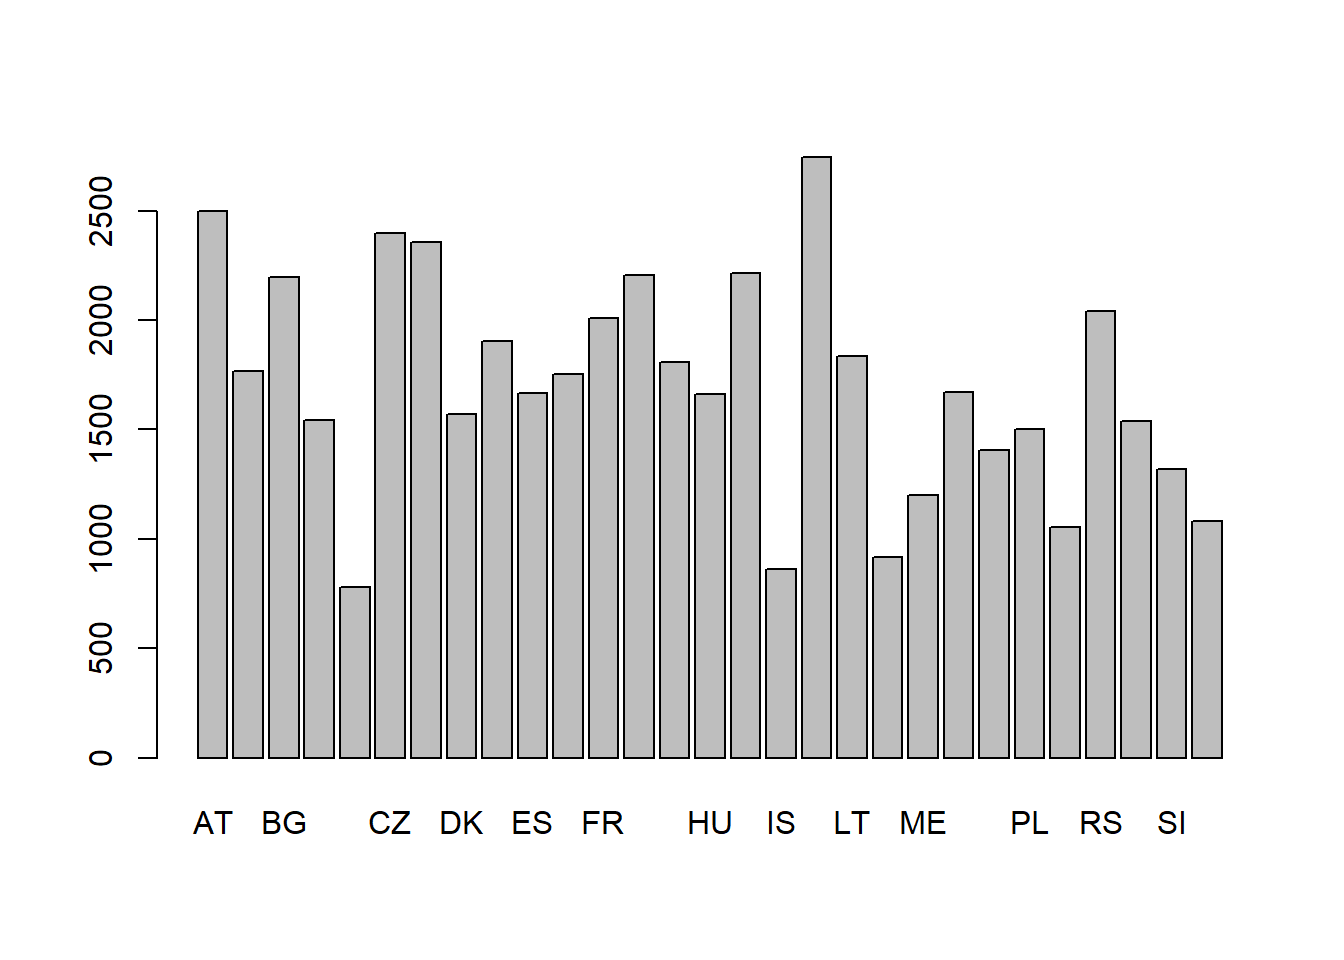
\includegraphics{bookdown-demo_files/figure-latex/unnamed-chunk-34-1.pdf}

\begin{verbatim}
## Country 
##       Frequency Percent
## AT         2499   5.047
## BE         1767   3.568
## BG         2198   4.439
## CH         1542   3.114
## CY          781   1.577
## CZ         2398   4.843
## DE         2358   4.762
## DK         1572   3.175
## EE         1904   3.845
## ES         1668   3.368
## FI         1755   3.544
## FR         2010   4.059
## GB         2204   4.451
## HR         1810   3.655
## HU         1661   3.354
## IE         2216   4.475
## IS          861   1.739
## IT         2745   5.543
## LT         1835   3.706
## LV          918   1.854
## ME         1200   2.423
## NL         1673   3.379
## NO         1406   2.839
## PL         1500   3.029
## PT         1055   2.130
## RS         2043   4.126
## SE         1539   3.108
## SI         1318   2.662
## SK         1083   2.187
## Total     49519 100.000
\end{verbatim}

On voit qu'il y a un certain nombre de pays, dont la Belgique, avec \(1767\) observations. Mais combien de pays y a-t-il exactement? R peut calculer cela pour vous. R comprend la fonction \href{https://www.rdocumentation.org/packages/base/versions/3.6.2/topics/unique}{\emph{unique()}} qui vous retourne les valeurs uniques sous forme de vecteur:

\begin{Shaded}
\begin{Highlighting}[]
\FunctionTok{unique}\NormalTok{(ESS9}\SpecialCharTok{$}\NormalTok{cntry)}
\end{Highlighting}
\end{Shaded}

\begin{verbatim}
## <labelled<character>[29]>: Country
##  [1] AT BE BG CH CY CZ DE DK EE ES FI FR GB HR HU IE IS IT LT LV ME NL NO PL PT RS SE SI SK
## 
## Labels:
##  value          label
##     AT        Austria
##     BE        Belgium
##     BG       Bulgaria
##     CH    Switzerland
##     CY         Cyprus
##     CZ        Czechia
##     DE        Germany
##     DK        Denmark
##     EE        Estonia
##     ES          Spain
##     FI        Finland
##     FR         France
##     GB United Kingdom
##     HR        Croatia
##     HU        Hungary
##     IE        Ireland
##     IS        Iceland
##     IT          Italy
##     LT      Lithuania
##     LV         Latvia
##     ME     Montenegro
##     NL    Netherlands
##     NO         Norway
##     PL         Poland
##     PT       Portugal
##     RS         Serbia
##     SE         Sweden
##     SI       Slovenia
##     SK       Slovakia
\end{verbatim}

Cela vous donne la liste des pays (ou plutôt des valeurs uniques) sous forme d'un nouveau vecteur. Cependant, cela ne vous informe pas sur leur nombre exact. Vous pouvez obtenir ce nombre par la fonction \emph{length()} qui compte le nombre d'éléments dans un vecteur. Vous pouvez l'appliquer soit en imbriquant les deux fonctions ainsi:

\begin{Shaded}
\begin{Highlighting}[]
\FunctionTok{length}\NormalTok{(}\FunctionTok{unique}\NormalTok{(ESS9}\SpecialCharTok{$}\NormalTok{cntry))}
\end{Highlighting}
\end{Shaded}

Vous pouvez aussi procéder en deux étapes en créant d'abord l'objet \emph{pays\_uniques}, reprenant la liste des pays sous forme de vecteur:

\begin{Shaded}
\begin{Highlighting}[]
\NormalTok{pays\_uniques}\OtherTok{\textless{}{-}}\FunctionTok{unique}\NormalTok{(ESS9}\SpecialCharTok{$}\NormalTok{cntry)}
\NormalTok{pays\_uniques}
\end{Highlighting}
\end{Shaded}

\begin{verbatim}
## <labelled<character>[29]>: Country
##  [1] AT BE BG CH CY CZ DE DK EE ES FI FR GB HR HU IE IS IT LT LV ME NL NO PL PT RS SE SI SK
## 
## Labels:
##  value          label
##     AT        Austria
##     BE        Belgium
##     BG       Bulgaria
##     CH    Switzerland
##     CY         Cyprus
##     CZ        Czechia
##     DE        Germany
##     DK        Denmark
##     EE        Estonia
##     ES          Spain
##     FI        Finland
##     FR         France
##     GB United Kingdom
##     HR        Croatia
##     HU        Hungary
##     IE        Ireland
##     IS        Iceland
##     IT          Italy
##     LT      Lithuania
##     LV         Latvia
##     ME     Montenegro
##     NL    Netherlands
##     NO         Norway
##     PL         Poland
##     PT       Portugal
##     RS         Serbia
##     SE         Sweden
##     SI       Slovenia
##     SK       Slovakia
\end{verbatim}

Puis, vous appliquez la fonction \emph{\href{https://www.rdocumentation.org/packages/base/versions/3.6.2/topics/length}{length()}} à l'objet \emph{pays\_uniques}. Cela vous donnera le nombre d'objets dans le vecteur \emph{pays\_uniques}, c'est-à-dire le nombre de pays dans la base de données \emph{ESS9}:

\begin{Shaded}
\begin{Highlighting}[]
\FunctionTok{length}\NormalTok{(pays\_uniques)}
\end{Highlighting}
\end{Shaded}

\begin{verbatim}
## [1] 29
\end{verbatim}

Cela nous indique, qu'il y a 29 pays dans la base de données \emph{ESS9}. Attention cependant: la fonction \emph{\href{https://www.rdocumentation.org/packages/base/versions/3.6.2/topics/length}{length()}} s'applique aux vecteurs ou listes, mais pas aux bases de données (\emph{data.frame} ou \emph{tibble}) ou matrices (\emph{matrix}). Si nous voulions connaître le nombre d'observations dans la base de données \emph{ESS9}, nous n'appliquons pas la fonction \emph{\href{https://www.rdocumentation.org/packages/base/versions/3.6.2/topics/length}{length()}}, mais la fonction \href{https://www.rdocumentation.org/packages/base/versions/3.6.2/topics/nrow}{\emph{nrow()}}, retournant le nombre de lignes (\emph{rows}) dans la base de données, ce qui revient à nous indiquer le nombre d'observations dans la base de données (vu que chaque ligne correspond à une observation):

\begin{Shaded}
\begin{Highlighting}[]
\FunctionTok{nrow}\NormalTok{(ESS9)}
\end{Highlighting}
\end{Shaded}

\begin{verbatim}
## [1] 49519
\end{verbatim}

Nous avons donc \(49519\) observations dans cette base de données. Mais comme nous l'avons expliqué, nous ne souhaitons pas analyser tous les pays, mais uniquement la Belgique. Pour continuer nos analyses, il faudra donc filtrer la base de données.

\hypertarget{filtrer-les-donnuxe9es}{%
\section{Filtrer les données}\label{filtrer-les-donnuxe9es}}

Vu que nous voulons analyser les salaires en Belgique, il faut sélectionner uniquement les observations belges. Pour sélectionner uniquement les observations belges, il faut vérifier quelle valeur dans la variable \emph{cntry} (\emph{Country}) de la base de données \emph{ESS9} (\emph{ESS9\$cntry} ) correspond à la Belgique. Nous pouvons faire cela en utilisant la fonction \href{https://www.rdocumentation.org/packages/labelled/versions/2.10.0/topics/val_labels}{\emph{val\_labels}} du \emph{package} \href{https://cran.r-project.org/web/packages/labelled/vignettes/intro_labelled.html}{\emph{labelled}}:

\begin{Shaded}
\begin{Highlighting}[]
\FunctionTok{val\_labels}\NormalTok{(ESS9}\SpecialCharTok{$}\NormalTok{cntry)}
\end{Highlighting}
\end{Shaded}

\begin{verbatim}
##        Austria        Belgium       Bulgaria    Switzerland         Cyprus        Czechia        Germany        Denmark        Estonia          Spain        Finland 
##           "AT"           "BE"           "BG"           "CH"           "CY"           "CZ"           "DE"           "DK"           "EE"           "ES"           "FI" 
##         France United Kingdom        Croatia        Hungary        Ireland        Iceland          Italy      Lithuania         Latvia     Montenegro    Netherlands 
##           "FR"           "GB"           "HR"           "HU"           "IE"           "IS"           "IT"           "LT"           "LV"           "ME"           "NL" 
##         Norway         Poland       Portugal         Serbia         Sweden       Slovenia       Slovakia 
##           "NO"           "PL"           "PT"           "RS"           "SE"           "SI"           "SK"
\end{verbatim}

Nous voyons que ``\emph{BE}'' correspond à la Belgique (\emph{Belgium}). Il faut donc garder uniquement les observations dont la variable \emph{cntry} (\emph{country}) est égale à ``BE''.

Il y a la fonction de base de R qui s'appelle \href{https://www.rdocumentation.org/packages/base/versions/3.6.2/topics/subset}{\emph{subset()}} qui permet de filtrer les observations sur un ou plusieurs critères. Nous allons cependant utiliser la fonction \href{https://dplyr.tidyverse.org/reference/filter.html}{\emph{filter()}} du \emph{package} \href{https://dplyr.tidyverse.org/}{\emph{dplyr}}\footnote{La fonction \href{https://www.rdocumentation.org/packages/base/versions/3.6.2/topics/subset}{\emph{subset()}} s'utilise de manière similaire à la fonction \emph{filter()}. Vous pouvez donc l'utiliser de manière analogue à la fonction \href{https://dplyr.tidyverse.org/reference/filter.html}{\emph{filter()}} présentée ici.}, faisant partie du \href{https://www.tidyverse.org/}{\emph{tidyverse}}, car celle-ci est facilement combinable avec d'autres manipulations.

Pour sélectionner uniquement les observations dont la variable \emph{cntry} est égale à ``\emph{BE}'', il faut utiliser la fonction \href{https://dplyr.tidyverse.org/reference/filter.html}{\emph{filter()}} de la manière suivante:

\begin{Shaded}
\begin{Highlighting}[]
\NormalTok{ESS9\_BE}\OtherTok{\textless{}{-}}\FunctionTok{filter}\NormalTok{(ESS9,cntry}\SpecialCharTok{==}\StringTok{"BE"}\NormalTok{)}
\end{Highlighting}
\end{Shaded}

On crée l'objet \emph{ESS9\_BE} contenant la base de données avec uniquement les cas belges. Comme vous le voyez, le premier argument de cette fonction \href{https://dplyr.tidyverse.org/reference/filter.html}{\emph{filter()}} est la base de données \emph{ESS9}. Puis, séparé par une virgule, le second argument est la condition à respecter. Ici, la condition est que la variable (colonne) \emph{cntry} doit être égale à ``BE''.

En lisant ce code, vous aurez certainement remarqué deux choses:

\begin{itemize}
\item
  La première est que ``BE'' est noté entre guillemets. En effet, lorsque vous filtrez des chaînes de caractère (\emph{string}/\emph{character}), il faut utiliser des guillemets autour des caractères que l'on souhaite filtrer. Si on n'utilise pas de guillemets, R pense qu'on lui indique un objet de nom \emph{BE}. Ne connaissant pas cet objet, R vous retournera une erreur. Entre guillemets, R sait que l'on veut dire la chaîne de caractère ``BE''. Si, en revanche, vous vouliez filtrer un nombre (par exemple: \(1\), \(1000\) ou \(1.35\)), vous n'avez pas besoin d'ajouter de guillemets (concrètement: vous ne devez \emph{pas} en mettre).
\item
  la deuxième est que l'on a indiqué un double égal (``==''). En effet, si l'on indique que l'on voudrait filtrer des éléments correspondant à ce qu'on indique (ici ``BE''), il faut indiquer un double égal (``=='').
\end{itemize}

R connaît ainsi un certain nombre d'opérateurs logiques:

\begin{itemize}
\tightlist
\item
  \(==\) : est égal à
\item
  \(!=\) : est différent de
\item
  \(!x\) : n'est pas x
\item
  \(%in%
  \) : est un des éléments dans la liste
\item
  \(<\) : est plus petit que
\item
  \(<=\) : est plus petit ou égal à
\item
  \(>\) : est plus grand que
\item
  \(>=\) : est plus grand ou égal à
\item
  \(x \& y\) : condition x \emph{ET} condition y
\item
  \(x | y\) : condition x \emph{OU} condition y
\end{itemize}

Prenons des exemples pour les deux derniers opérateurs de la liste ``\&'' et ``\textbar{}'' :

\begin{itemize}
\tightlist
\item
  Imaginons que vous vouliez garder les observations en Belgique, mais uniquement si elles sont des femmes: dans ce cas si vous utilisiez le lien logique ``\&'' ente les conditions. Cela signifierait que les deux conditions doivent être remplies simultanément. Les observations sélectionnées doivent être en Belgique \emph{ET} des femmes. Les observations en Belgique qui ne sont pas des femmes ou les femmes qui ne sont pas en Belgique ne seront pas sélectionnées. Le code serait alors:
\end{itemize}

\begin{Shaded}
\begin{Highlighting}[]
\NormalTok{ESS9\_BE\_Women}\OtherTok{\textless{}{-}}\FunctionTok{filter}\NormalTok{(ESS9,cntry}\SpecialCharTok{==}\StringTok{"BE"} \SpecialCharTok{\&}\NormalTok{ gndr}\SpecialCharTok{==}\DecValTok{2}\NormalTok{)}

\CommentTok{\#Regardez le résultat:}
\FunctionTok{freq}\NormalTok{(ESS9\_BE\_Women}\SpecialCharTok{$}\NormalTok{cntry)}
\end{Highlighting}
\end{Shaded}

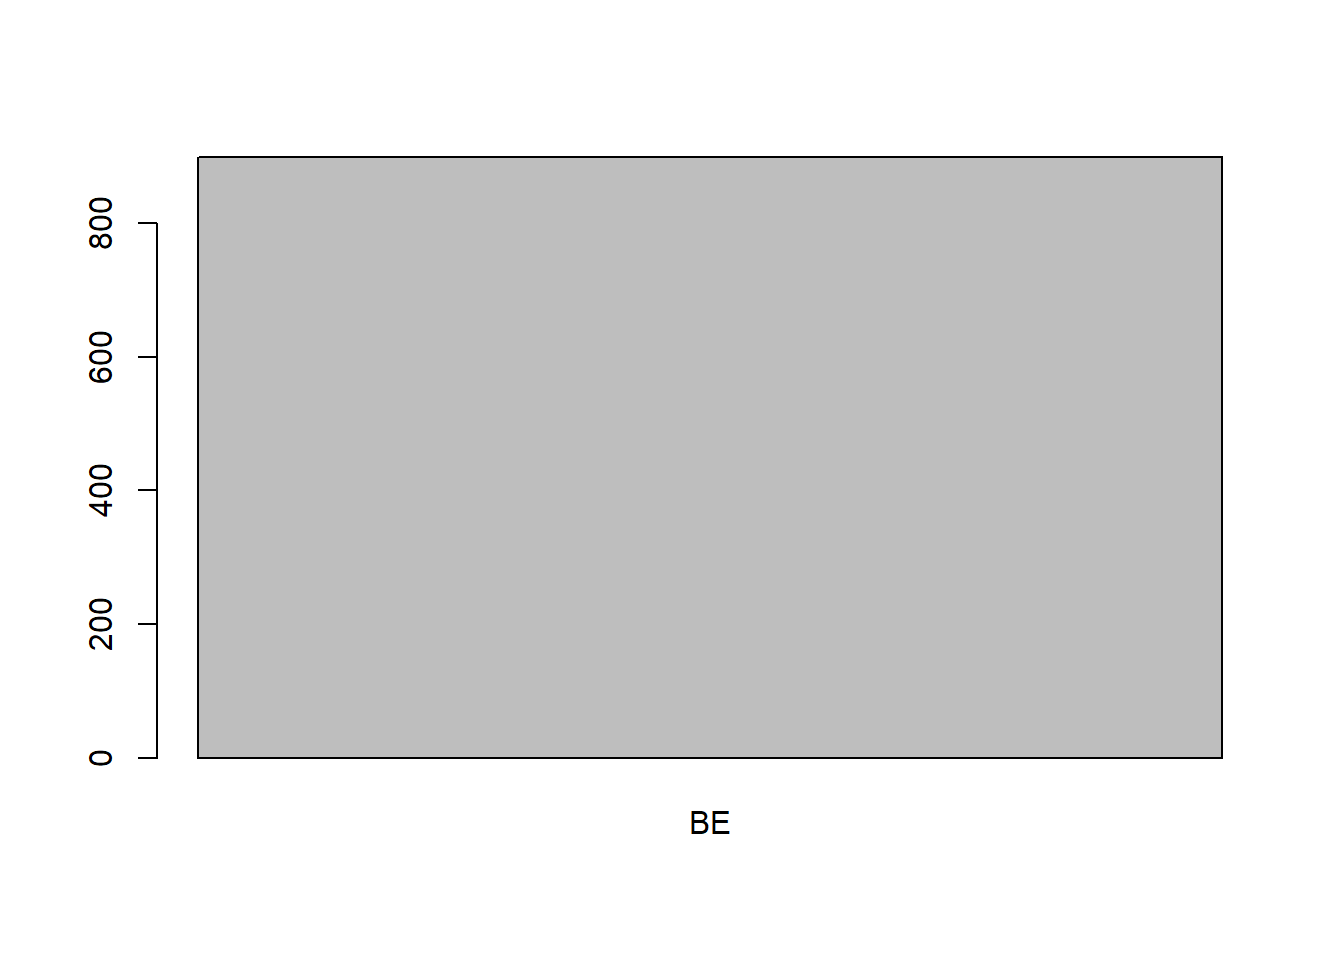
\includegraphics{bookdown-demo_files/figure-latex/unnamed-chunk-42-1.pdf}

\begin{verbatim}
## Country 
##       Frequency Percent
## BE          899     100
## Total       899     100
\end{verbatim}

\begin{Shaded}
\begin{Highlighting}[]
\FunctionTok{freq}\NormalTok{(ESS9\_BE\_Women}\SpecialCharTok{$}\NormalTok{gndr)}
\end{Highlighting}
\end{Shaded}

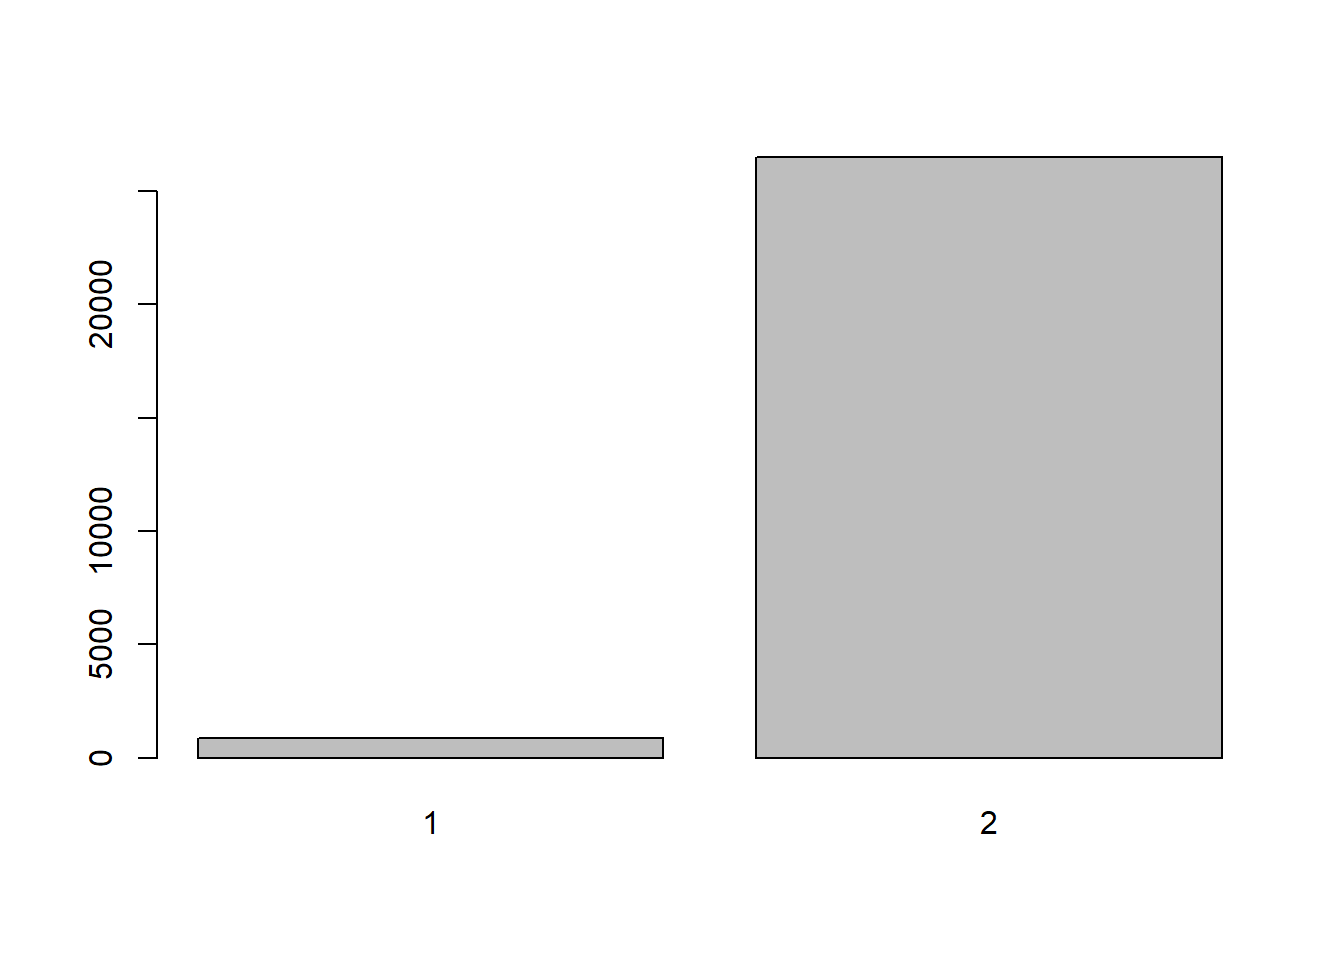
\includegraphics{bookdown-demo_files/figure-latex/unnamed-chunk-42-2.pdf}

\begin{verbatim}
## Gender 
##       Frequency Percent
## 2           899     100
## Total       899     100
\end{verbatim}

\begin{itemize}
\tightlist
\item
  Imaginons que vous vouliez garder toutes les observations en Belgique et toutes les femmes: dans ce cas, vous devriez séparer les deux conditions par le symbole ``\textbar{}''. Les observations sélectionnées doivent être en Belgique \emph{OU} des femmes. Toutes les observations belges sont alors sélectionnées et toutes les observations ``femmes''. Les observations en Belgique qui ne sont pas des femmes seront sélectionnées tout comme les femmes qui ne sont pas en Belgique. Le code serait alors:
\end{itemize}

\begin{Shaded}
\begin{Highlighting}[]
\NormalTok{ESS9\_BE\_OR\_Women}\OtherTok{\textless{}{-}}\FunctionTok{filter}\NormalTok{(ESS9,cntry}\SpecialCharTok{==}\StringTok{"BE"} \SpecialCharTok{|}\NormalTok{ gndr}\SpecialCharTok{==}\DecValTok{2}\NormalTok{)}

\CommentTok{\#Regardez le résultat:}
\FunctionTok{freq}\NormalTok{(ESS9\_BE\_OR\_Women}\SpecialCharTok{$}\NormalTok{cntry)}
\end{Highlighting}
\end{Shaded}

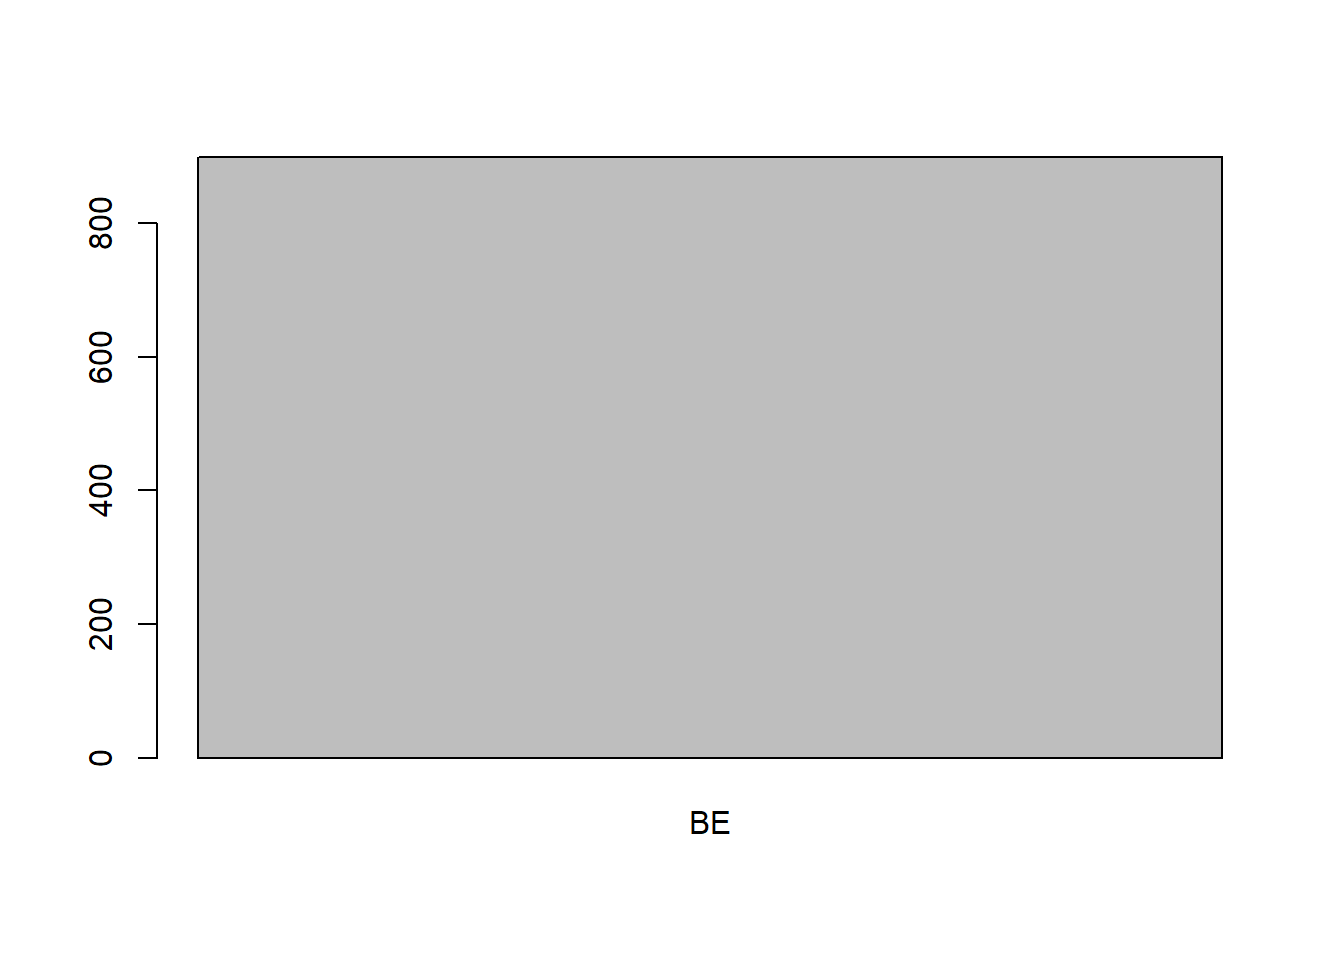
\includegraphics{bookdown-demo_files/figure-latex/unnamed-chunk-43-1.pdf}

\begin{verbatim}
## Country 
##       Frequency Percent
## AT         1346   4.918
## BE         1767   6.457
## BG         1222   4.465
## CH          767   2.803
## CY          415   1.516
## CZ         1349   4.929
## DE         1146   4.188
## DK          726   2.653
## EE         1067   3.899
## ES          821   3.000
## FI          907   3.314
## FR         1097   4.008
## GB         1206   4.407
## HR         1082   3.954
## HU          955   3.490
## IE         1161   4.242
## IS          440   1.608
## IT         1447   5.287
## LT         1261   4.608
## LV          621   2.269
## ME          592   2.163
## NL          840   3.069
## NO          629   2.298
## PL          790   2.887
## PT          610   2.229
## RS         1058   3.866
## SE          757   2.766
## SI          708   2.587
## SK          580   2.119
## Total     27367 100.000
\end{verbatim}

\begin{Shaded}
\begin{Highlighting}[]
\FunctionTok{freq}\NormalTok{(ESS9\_BE\_OR\_Women}\SpecialCharTok{$}\NormalTok{gndr)}
\end{Highlighting}
\end{Shaded}

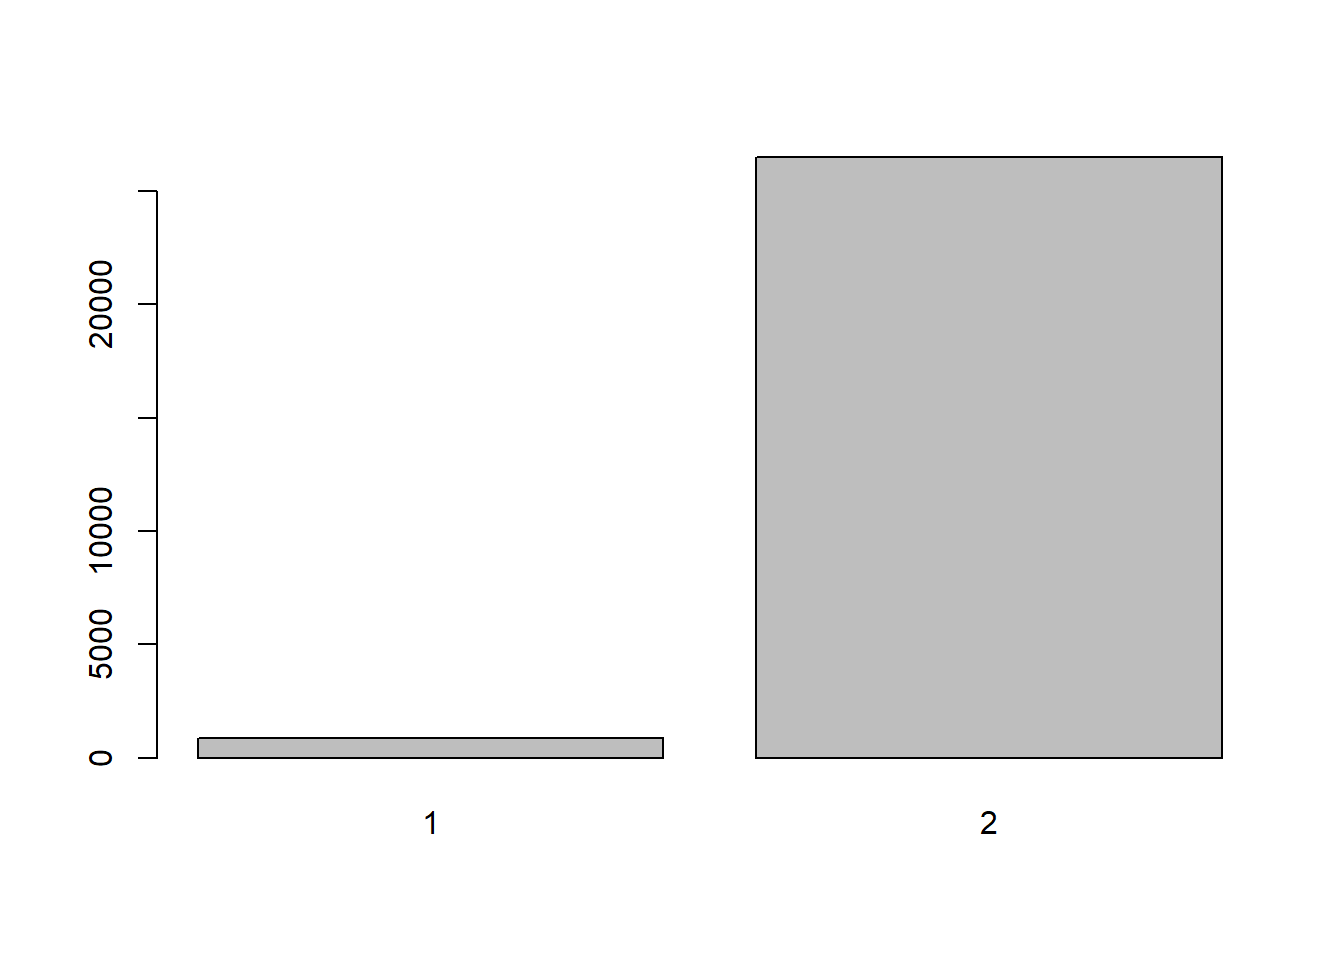
\includegraphics{bookdown-demo_files/figure-latex/unnamed-chunk-43-2.pdf}

\begin{verbatim}
## Gender 
##       Frequency Percent
## 1           868   3.172
## 2         26499  96.828
## Total     27367 100.000
\end{verbatim}

Une fois que nous avons exécuté la fonction \href{https://dplyr.tidyverse.org/reference/filter.html}{\emph{filter()}} pour garder uniquement les observations en Belgique créant la base de données nommée \emph{ESS9\_BE}, nous allons vérifier qu'elle contient plus que des observations belges avec la fonction \href{https://www.rdocumentation.org/packages/base/versions/3.6.2/topics/table}{\emph{table()}} et \href{https://www.rdocumentation.org/packages/descr/versions/1.1.5/topics/freq}{\emph{freq()}}:

\begin{Shaded}
\begin{Highlighting}[]
\NormalTok{ESS9\_BE}\OtherTok{\textless{}{-}}\FunctionTok{filter}\NormalTok{(ESS9,cntry}\SpecialCharTok{==}\StringTok{"BE"}\NormalTok{)}

\FunctionTok{table}\NormalTok{(ESS9\_BE}\SpecialCharTok{$}\NormalTok{cntry) }\CommentTok{\# Attention à bien sélectionner la base de données ESS9\_BE}
\end{Highlighting}
\end{Shaded}

\begin{verbatim}
## 
##   BE 
## 1767
\end{verbatim}

\begin{Shaded}
\begin{Highlighting}[]
\FunctionTok{freq}\NormalTok{(ESS9\_BE}\SpecialCharTok{$}\NormalTok{cntry) }\CommentTok{\# Attention à bien sélectionner la base de données ESS9\_BE}
\end{Highlighting}
\end{Shaded}

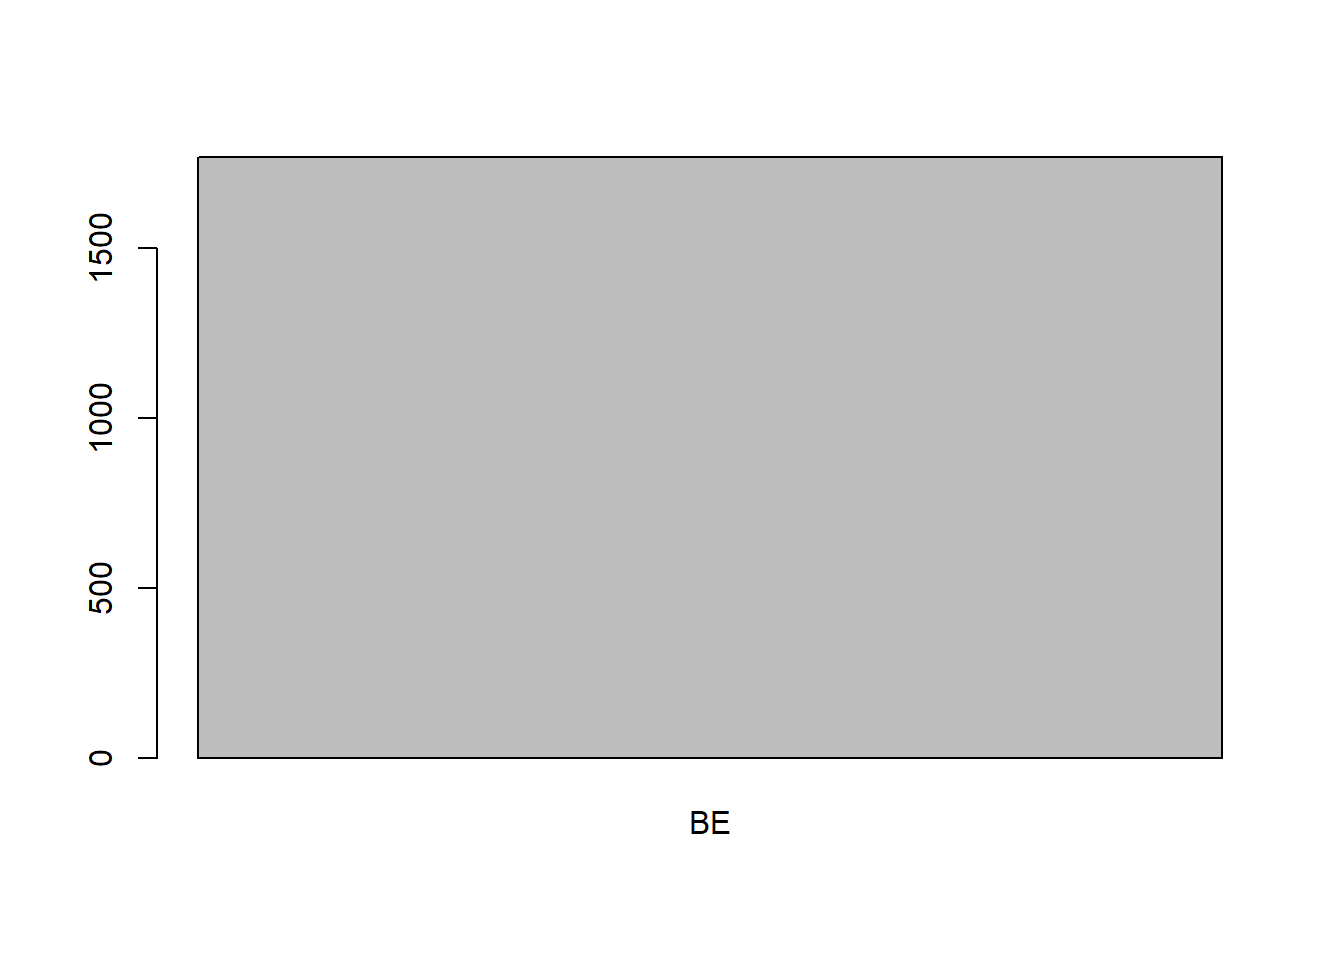
\includegraphics{bookdown-demo_files/figure-latex/unnamed-chunk-44-1.pdf}

\begin{verbatim}
## Country 
##       Frequency Percent
## BE         1767     100
## Total      1767     100
\end{verbatim}

Comme nous le voyons, le filtrage a fonctionné: il n'y plus que \(1767\) observations belges. Nous pouvons donc procéder à une analyse descriptive des salaires en Belgique dans le \protect\hyperlink{salaire_belge_stat_desc}{chapitre suivant}.

\hypertarget{salaire_belge_stat_desc}{%
\chapter{Le salaire de Belges}\label{salaire_belge_stat_desc}}

Si vous avez fermé R depuis le dernier chapitre, il faudra lancer les \emph{packages}. Vous pouvez le faire avec le code suivant:

\begin{Shaded}
\begin{Highlighting}[]
\ControlFlowTok{if}\NormalTok{ (}\SpecialCharTok{!}\FunctionTok{require}\NormalTok{(}\StringTok{"pacman"}\NormalTok{)) }\FunctionTok{install.packages}\NormalTok{(}\StringTok{"pacman"}\NormalTok{) }\CommentTok{\#Cela vérifie}
                             \CommentTok{\#si le package pacman est installé.}
                             \CommentTok{\#S\textquotesingle{}il ne l\textquotesingle{}est pas, il est installé.}

\NormalTok{pacman}\SpecialCharTok{::}\FunctionTok{p\_load}\NormalTok{(tidyverse, descr, rcompanion, codebook,}
\NormalTok{               DT, sjPlot, labelled) }\CommentTok{\#On lance les packages}
\end{Highlighting}
\end{Shaded}

\hypertarget{statistiques-descriptives-et-simples-graphiques-des-salaires-des-belges}{%
\section{Statistiques descriptives et simples graphiques des salaires des Belges}\label{statistiques-descriptives-et-simples-graphiques-des-salaires-des-belges}}

Si l'on veut étudier les salaires des Belges il faut que nous continuions à travailler avec la base de données \emph{ESS9\_BE} que nous avons créée dans le \protect\hyperlink{charge_code_filtrer}{chapitre précédent} précédemment qui contient exclusivement les observations belges. Par ailleurs, il faut que nous identifiions la variable de la base de données contenant les salaires. Il s'agit de la variable \emph{grspnum}. Nous pouvons obtenir des statistiques descriptives de cette variable avec la commande \href{https://www.rdocumentation.org/packages/base/versions/3.6.2/topics/summary}{\emph{summary()}}:

\begin{Shaded}
\begin{Highlighting}[]
\FunctionTok{summary}\NormalTok{(ESS9\_BE}\SpecialCharTok{$}\NormalTok{grspnum)}
\end{Highlighting}
\end{Shaded}

\begin{verbatim}
##    Min. 1st Qu.  Median    Mean 3rd Qu.    Max.    NA's 
##       0    2019    2800    3148    3700   40000    1068
\end{verbatim}

On voit que la valeur minimale est de \(0€\), la valeur maximale de \(40000€\). La moyenne s'élève à \(3148€\) tandis que la médiane est sensiblement plus basse à \(2800€\). Cela suggère qu'un nombre restreint de valeurs très élevées tirent la moyenne vers le haut. Il est à noter qu'il y a un nombre important de valeurs manquantes: \(1068\), soit \(60\%\) sur les \(1767\).

Faisons-nous une image de cette distribution. Vu qu'il s'agit d'une variable continue, nous représentons ceci sous forme d'histogramme avec la fonction de base \href{https://www.rdocumentation.org/packages/graphics/versions/3.6.2/topics/hist}{\emph{hist()}} et la fonction un peu plus avancée \href{https://www.rdocumentation.org/packages/rcompanion/versions/2.4.21/topics/plotNormalHistogram}{\emph{plotNormalHistogram}} du \emph{package} \href{https://rcompanion.org/handbook/}{rcompanion} y ajoutant une courbe de distribution normale (``cloche'')\footnote{Nous définissions qu'il y a 50 barres dans l'histogramme: ``breaks = 50'' comme second argument de la fonction \href{https://www.rdocumentation.org/packages/graphics/versions/3.6.2/topics/hist}{\emph{hist()}} et \href{https://www.rdocumentation.org/packages/rcompanion/versions/2.4.21/topics/plotNormalHistogram}{\emph{plotNormalHistogram}}.}:

\begin{Shaded}
\begin{Highlighting}[]
\FunctionTok{hist}\NormalTok{(ESS9\_BE}\SpecialCharTok{$}\NormalTok{grspnum, }\AttributeTok{breaks =} \DecValTok{50}\NormalTok{)}
\end{Highlighting}
\end{Shaded}

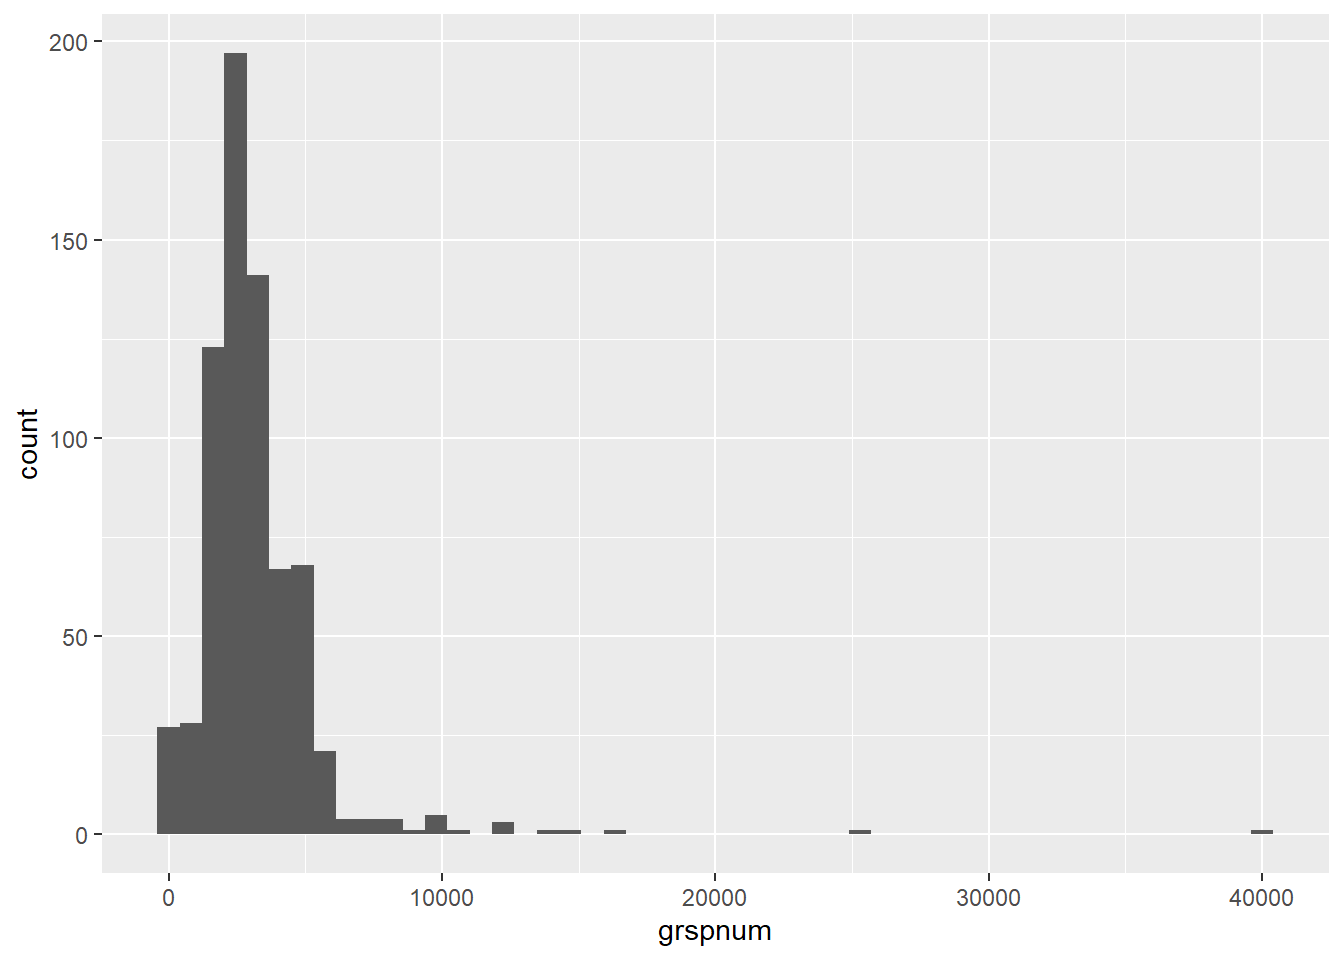
\includegraphics{bookdown-demo_files/figure-latex/unnamed-chunk-47-1.pdf}

\begin{Shaded}
\begin{Highlighting}[]
\FunctionTok{plotNormalHistogram}\NormalTok{(ESS9\_BE}\SpecialCharTok{$}\NormalTok{grspnum,}
                    \AttributeTok{breaks =} \DecValTok{50}\NormalTok{)}
\end{Highlighting}
\end{Shaded}

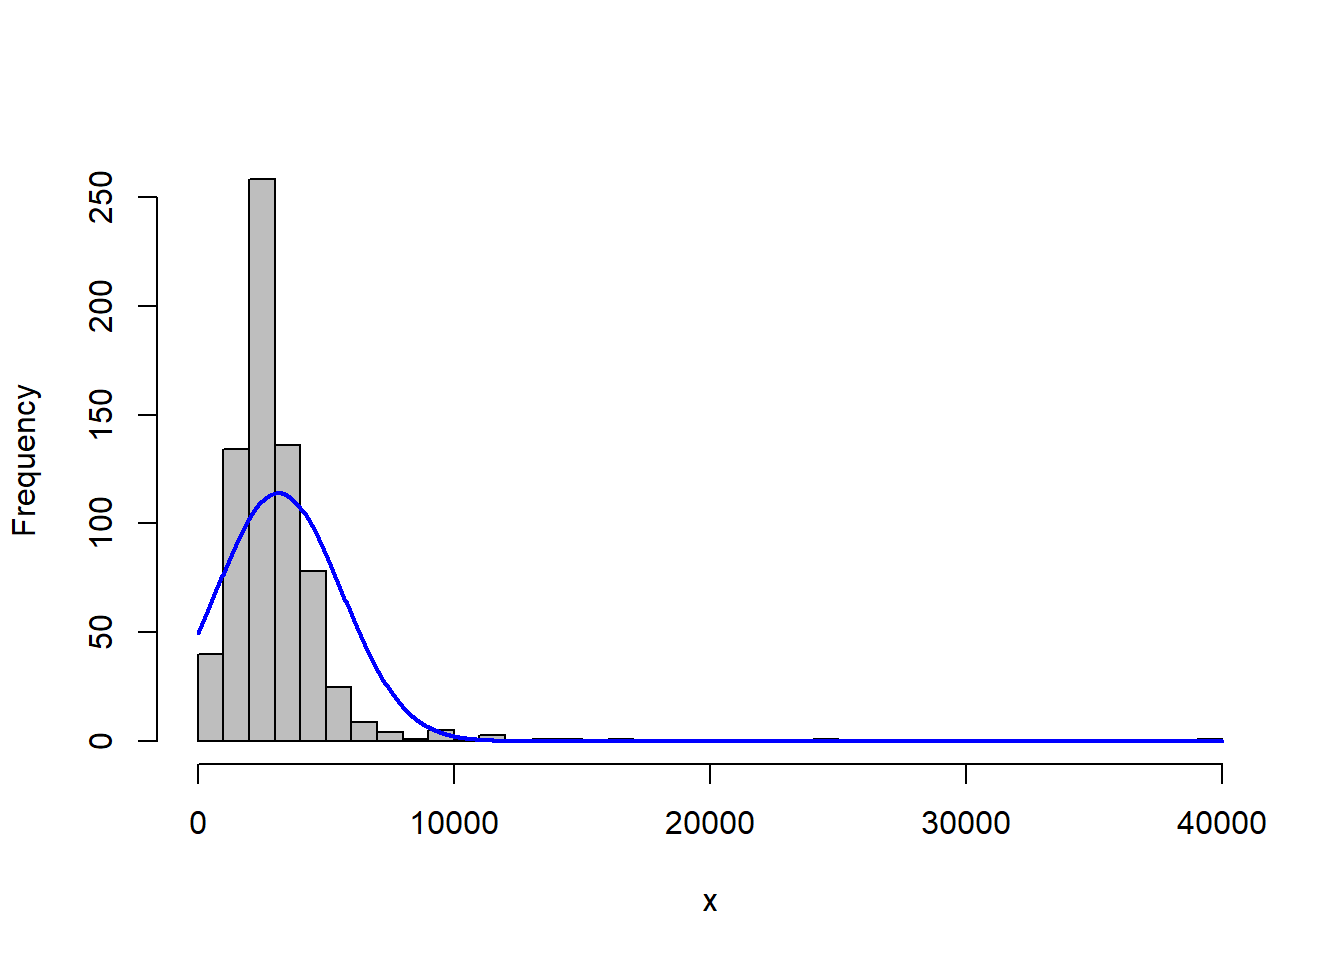
\includegraphics{bookdown-demo_files/figure-latex/unnamed-chunk-47-2.pdf}

On peut aussi faire de graphiques plus attrayants avec les fonctions du \emph{package} \href{https://ggplot2.tidyverse.org/}{\emph{ggplot2}} de l'ensemble \href{https://www.tidyverse.org/}{\emph{tidyverse}}\footnote{Nous définissons qu'il y a 50 barres dans l'histogramme: ``bins=50'' comme second argument de la fonction \href{https://ggplot2.tidyverse.org/reference/geom_histogram.html}{\emph{geom\_histogram}}.}:

\begin{Shaded}
\begin{Highlighting}[]
\FunctionTok{ggplot}\NormalTok{(ESS9\_BE, }\FunctionTok{aes}\NormalTok{(}\AttributeTok{x=}\NormalTok{grspnum)) }\SpecialCharTok{+}
  \FunctionTok{geom\_histogram}\NormalTok{(}\AttributeTok{bins=}\DecValTok{50}\NormalTok{)}
\end{Highlighting}
\end{Shaded}

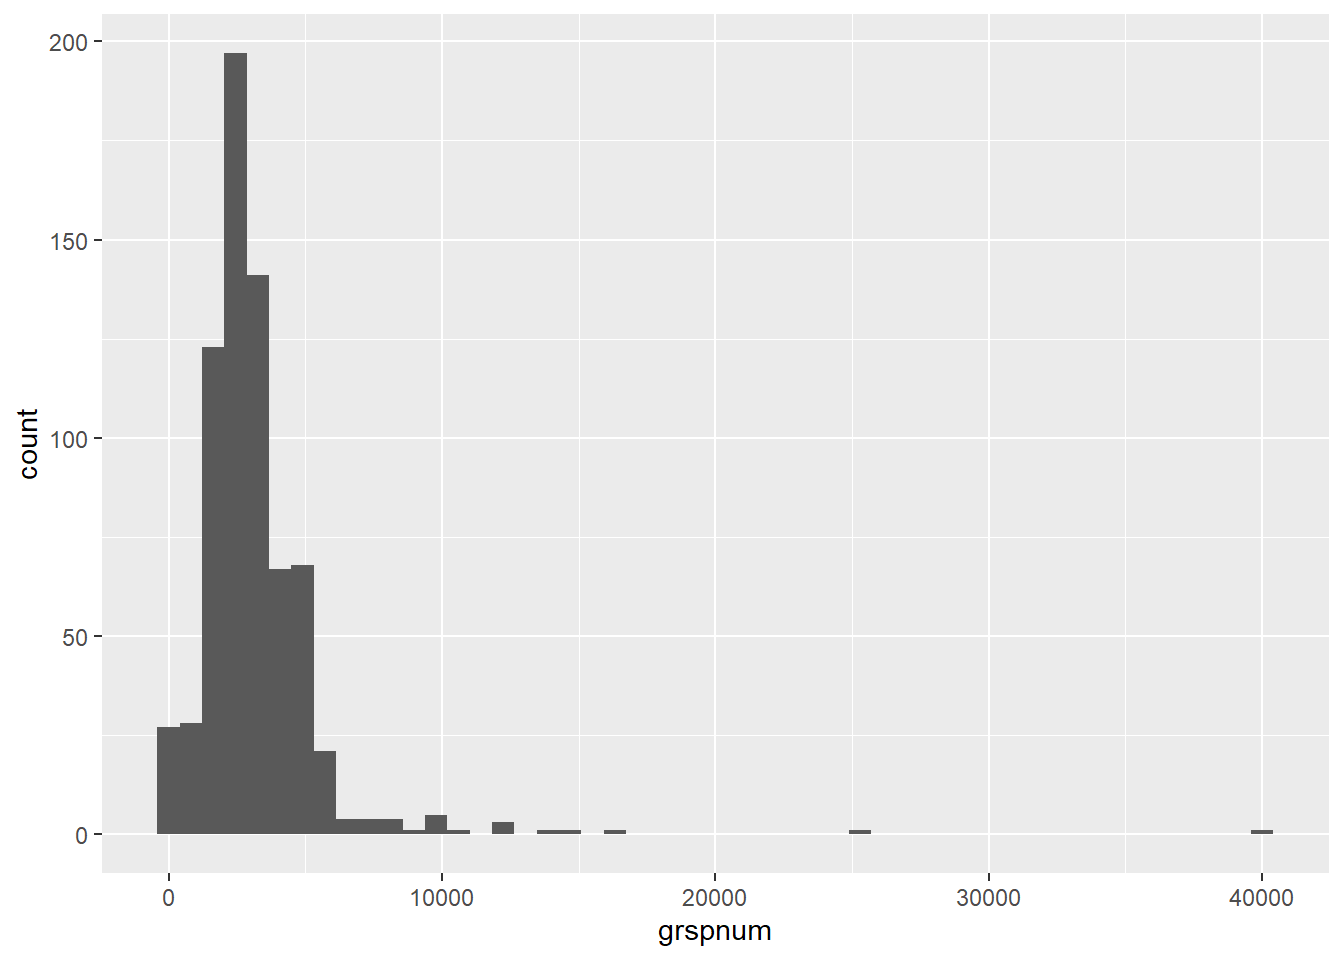
\includegraphics{bookdown-demo_files/figure-latex/unnamed-chunk-48-1.pdf}

On voit très clairement que la plupart des valeurs sont concentrées entre \(0€\) et \(5000€\) et qu'au-delà de \(10000\) il n'y a plus que quelques observations isolées. Celles-ci tirent la moyenne vers le haut. Un autre moyen de représenter cela est de le faire à l'aide d'une ``boîte à moustache'' (\emph{boxplot}):

\begin{Shaded}
\begin{Highlighting}[]
\FunctionTok{boxplot}\NormalTok{(ESS9\_BE}\SpecialCharTok{$}\NormalTok{grspnum)}
\end{Highlighting}
\end{Shaded}

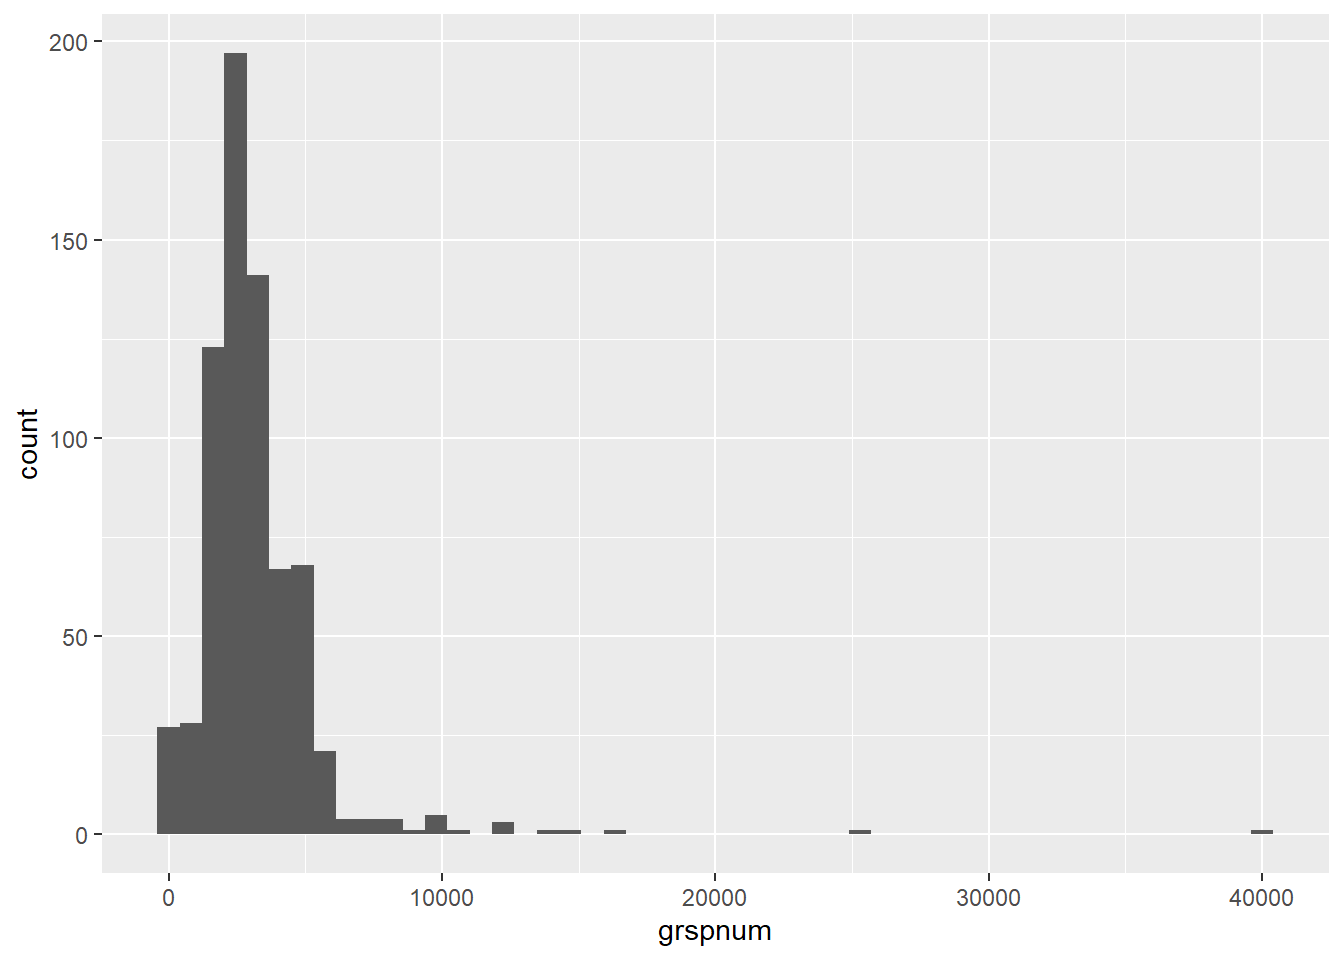
\includegraphics{bookdown-demo_files/figure-latex/unnamed-chunk-49-1.pdf}

Vous pouvez aussi la représenter à l'aide de du \emph{package} \href{https://ggplot2.tidyverse.org/}{\emph{ggplot2}}\footnote{Si vous comparer le code du \emph{boxplot} à l'histogramme avec \href{https://ggplot2.tidyverse.org/}{\emph{ggplot2}}, vous remarquerez, que seule la deuxième partie de la commande a changée. Cette similarité du code est un grand avantage du \emph{package} \href{https://ggplot2.tidyverse.org/}{\emph{ggplot2}}. Nous reviendrons plus tard sur la syntaxe et l'utilisation de \href{https://ggplot2.tidyverse.org/}{\emph{ggplot2}}.}:

\begin{Shaded}
\begin{Highlighting}[]
\FunctionTok{ggplot}\NormalTok{(ESS9\_BE, }\FunctionTok{aes}\NormalTok{(}\AttributeTok{x=}\NormalTok{grspnum)) }\SpecialCharTok{+}
  \FunctionTok{geom\_boxplot}\NormalTok{()}
\end{Highlighting}
\end{Shaded}

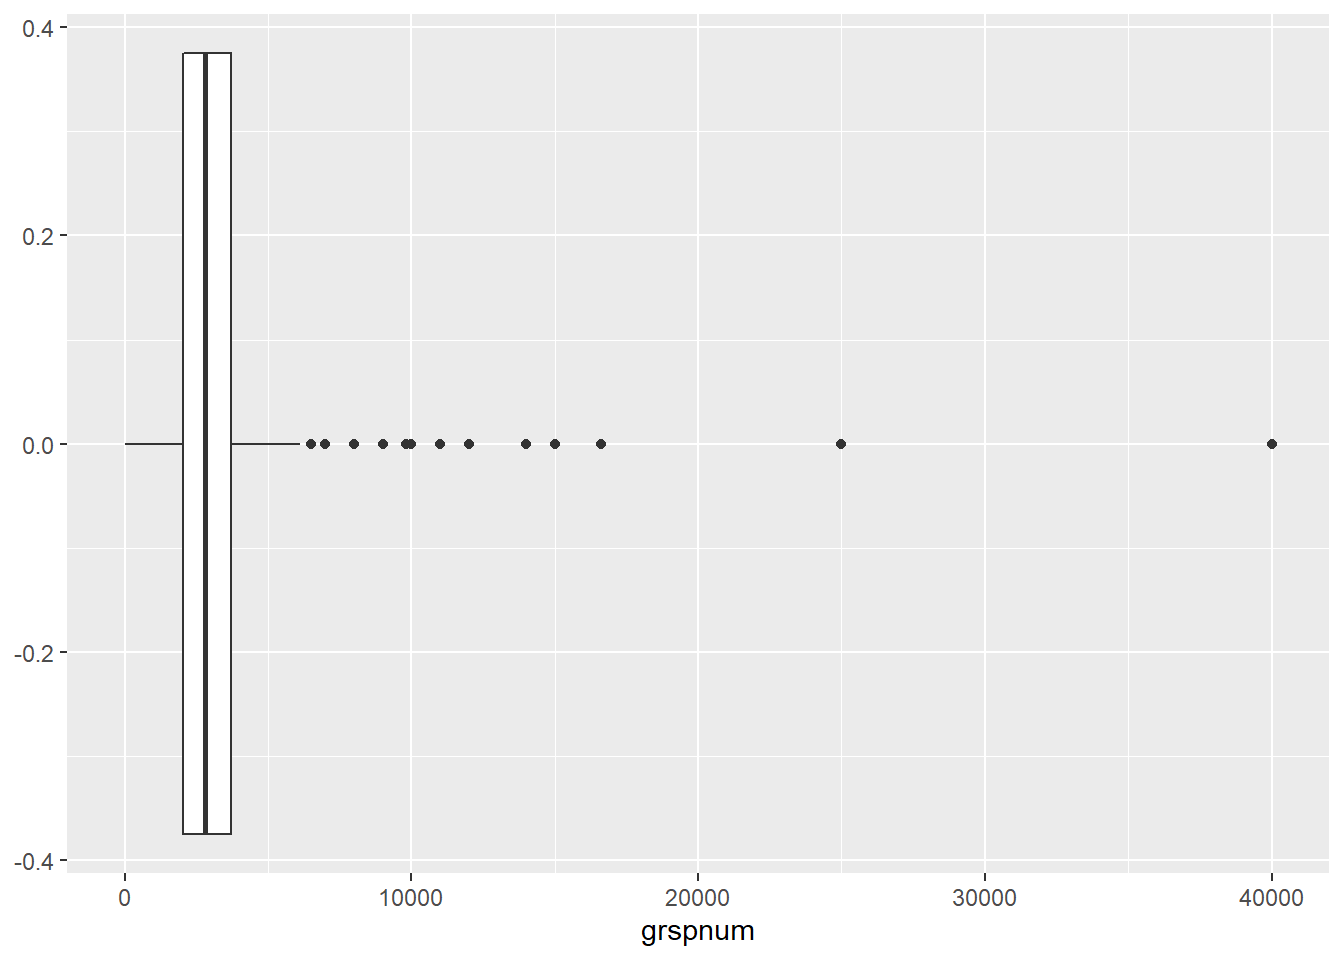
\includegraphics{bookdown-demo_files/figure-latex/unnamed-chunk-50-1.pdf}

Les \emph{boxplots} indiquent aussi très clairement qu'il y a quelques valeurs ``extrêmes'', très élevées, qui ``tirent'' la moyenne vers le haut. Par ailleurs, il y a un certain nombre d'observations avec des revenus très faibles, tels que \(0€\).

Il nous semble utile de considérer seulement les personnes travaillant à temps plein. Par ailleurs, il faut contrôler que les données soient cohérentes. La Belgique ayant un salaire minimum, il n'est pas légalement possible pour un salarié de percevoir un salaire de moins de \(1000€\) tout en travaillant à temps plein\footnote{Il est certainement possible qu'il y ait des cas très spécifiques où cela puisse se produire. Mais nous excluons ces cas de nos analyses.}.

Nous nous concentrons ainsi sur les Belges travaillant plus de 34 heures pas semaine (temps plein) et gagnant plus de \(1000€\) par mois, mais moins de \(15000€\) par mois. La variable ``\emph{wkhtot}'' indique le nombre d'heures travaillées par semaine. On utilise la fonction \href{https://dplyr.tidyverse.org/reference/filter.html}{\emph{filter()}} pour sélectionner les observations. On crée une nouvelle base de données nommée \emph{ESS9\_BE\_fulltime}:

\begin{Shaded}
\begin{Highlighting}[]
\NormalTok{ESS9\_BE\_fulltime}\OtherTok{\textless{}{-}}\FunctionTok{filter}\NormalTok{(ESS9\_BE, }\CommentTok{\#Base de donnés}
\NormalTok{                   wkhtot}\SpecialCharTok{\textgreater{}}\DecValTok{34} \SpecialCharTok{\&} \CommentTok{\# Travaillant plus de 34 heures}
\NormalTok{                     grspnum}\SpecialCharTok{\textgreater{}}\DecValTok{1000} \SpecialCharTok{\&} \CommentTok{\# Percevant plus de 1000€,}
\NormalTok{                     grspnum}\SpecialCharTok{\textless{}}\DecValTok{15000}\NormalTok{) }\CommentTok{\# mais moins de 15.000€.}
\end{Highlighting}
\end{Shaded}

Vous pouvez vérifier cette base de données, notamment en vous assurant qu'il n'y a personne qui ravitaille moins de 35 heures et percevant moins de \(1000€\) et plus de \(15000€\). Vous pouvez utiliser la fonction \href{https://www.rdocumentation.org/packages/base/versions/3.6.2/topics/summary}{\emph{summary()}} pour vérifier que les variables \emph{grspnum} et \emph{wkhtot} dans la base de données \emph{ESS9\_BE\_fulltime} ne contiennent plus que des valeurs compatibles avec le filtre que l'on vient d'appliquer:

\begin{Shaded}
\begin{Highlighting}[]
\FunctionTok{summary}\NormalTok{(ESS9\_BE\_fulltime}\SpecialCharTok{$}\NormalTok{grspnum)}
\end{Highlighting}
\end{Shaded}

\begin{verbatim}
##    Min. 1st Qu.  Median    Mean 3rd Qu.    Max. 
##    1200    2400    2986    3365    4000   14000
\end{verbatim}

\begin{Shaded}
\begin{Highlighting}[]
\FunctionTok{summary}\NormalTok{(ESS9\_BE\_fulltime}\SpecialCharTok{$}\NormalTok{wkhtot)}
\end{Highlighting}
\end{Shaded}

\begin{verbatim}
##    Min. 1st Qu.  Median    Mean 3rd Qu.    Max. 
##   35.00   38.00   40.00   45.58   46.00  168.00
\end{verbatim}

Le filtrage a fonctionné: dans notre échantillon, personne ne travaille moins de 35 heures et personne ne perçoit moins de \(1000€\) (le minimum est de \(1200€\)) et plus de \(15000€\) (le maximum est \(14000€\)). Cependant, des anomalies apparaissent au niveau du temps de travail. L'on peut s'en rendre compte avec les fonctions \href{https://www.rdocumentation.org/packages/base/versions/3.6.2/topics/table}{\emph{table()}} et \href{https://www.rdocumentation.org/packages/descr/versions/1.1.5/topics/freq}{\emph{freq()}}:

\begin{Shaded}
\begin{Highlighting}[]
\FunctionTok{table}\NormalTok{(ESS9\_BE\_fulltime}\SpecialCharTok{$}\NormalTok{wkhtot)}
\end{Highlighting}
\end{Shaded}

\begin{verbatim}
## 
##  35  36  37  38  39  40  41  42  43  44  45  46  47  48  49  50  52  53  55  56  60  62  65  70  72  75  80  84 100 105 147 168 
##  19  12  13 110  18 103   9  23   9   8  67   4   3   7   1  48   1   1   8   1  24   1   6  13   2   4   3   1   1   1   1   4
\end{verbatim}

\begin{Shaded}
\begin{Highlighting}[]
\FunctionTok{freq}\NormalTok{(ESS9\_BE\_fulltime}\SpecialCharTok{$}\NormalTok{wkhtot)}
\end{Highlighting}
\end{Shaded}

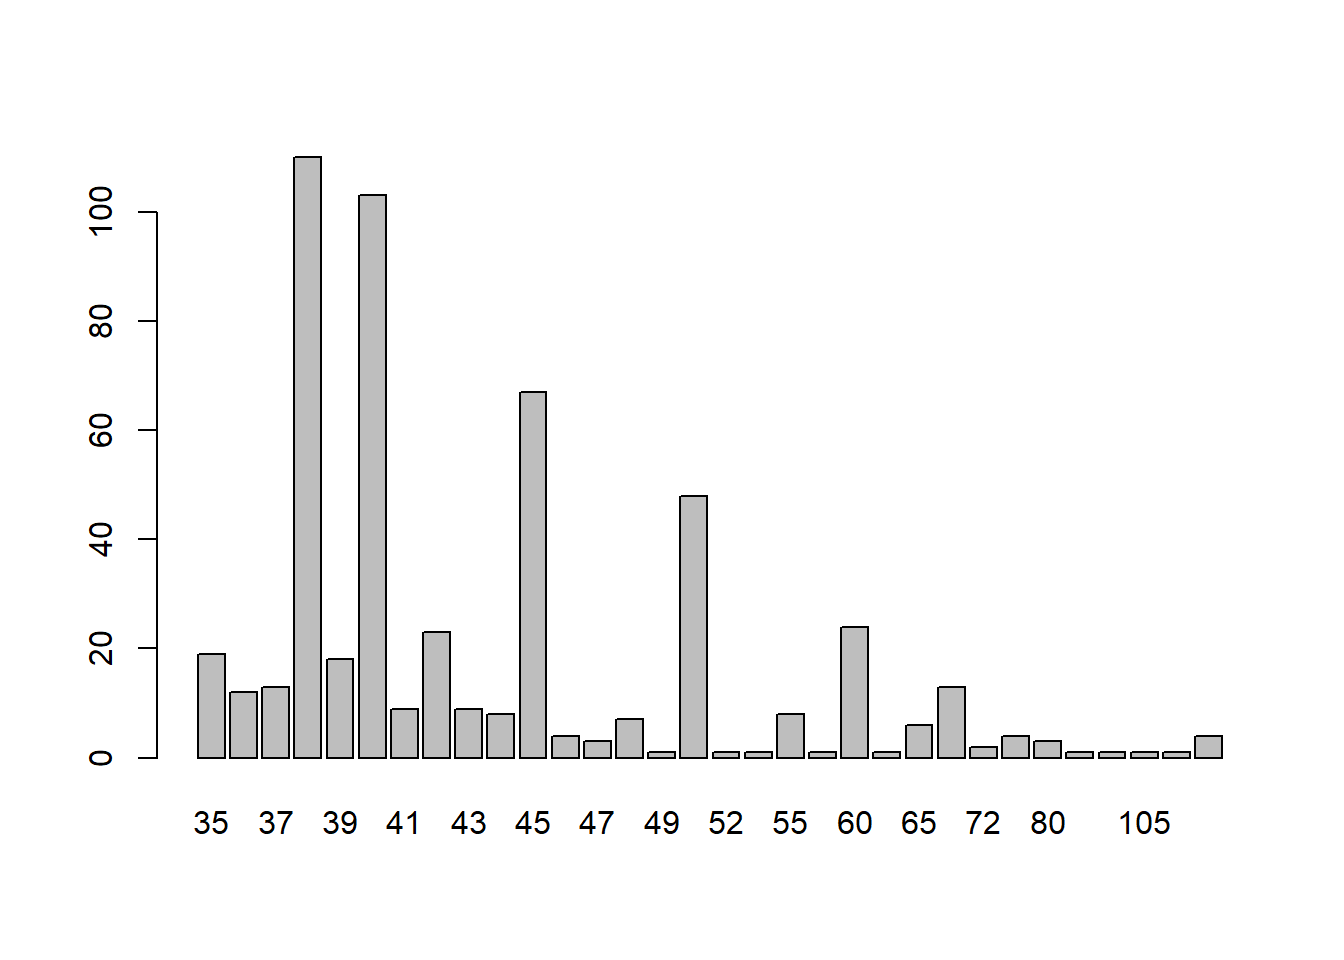
\includegraphics{bookdown-demo_files/figure-latex/unnamed-chunk-53-1.pdf}

\begin{verbatim}
## Total hours normally worked per week in main job overtime included 
##       Frequency  Percent
## 35           19   3.6122
## 36           12   2.2814
## 37           13   2.4715
## 38          110  20.9125
## 39           18   3.4221
## 40          103  19.5817
## 41            9   1.7110
## 42           23   4.3726
## 43            9   1.7110
## 44            8   1.5209
## 45           67  12.7376
## 46            4   0.7605
## 47            3   0.5703
## 48            7   1.3308
## 49            1   0.1901
## 50           48   9.1255
## 52            1   0.1901
## 53            1   0.1901
## 55            8   1.5209
## 56            1   0.1901
## 60           24   4.5627
## 62            1   0.1901
## 65            6   1.1407
## 70           13   2.4715
## 72            2   0.3802
## 75            4   0.7605
## 80            3   0.5703
## 84            1   0.1901
## 100           1   0.1901
## 105           1   0.1901
## 147           1   0.1901
## 168           4   0.7605
## Total       526 100.0000
\end{verbatim}

Ainsi 4 répondants affirment travailler \(168\) heures par semaine. Vu qu'une semaine compte \(168\) heures et que l'être humain a un besoin physiologique de sommeil, ces réponses semblent aberrantes\footnote{Il faudrait analyser plus en détail ces cas anormaux: peut-être que les personnes concernées exercent des professions en tant qu'indépendants et s'estiment ``de garde'' en permanence.}. Vue que l'analyse que nous voulons mener ne porte pas sur le temps de travail, nous n'allons ni investiguer ces cas plus en détail, ni les exclure de nos analyses.

La distribution de la variable dans la base de données que nous avons filtrée, se rapproche-t-elle d'une distribution normale? Analysons cela à nouveau avec les histogrammes et ``boxplots'':

\begin{Shaded}
\begin{Highlighting}[]
\CommentTok{\#Avec R de base:}

\FunctionTok{hist}\NormalTok{(ESS9\_BE\_fulltime}\SpecialCharTok{$}\NormalTok{grspnum,}
     \AttributeTok{breaks =} \DecValTok{50}\NormalTok{,}
     \AttributeTok{main=}\StringTok{"Histogramme: Salaire des Belges en 2018"}\NormalTok{,}
     \AttributeTok{xlab=}\StringTok{"Salaire des Belges en €"}\NormalTok{)}

\CommentTok{\#Avec ggplot2:}

\NormalTok{ESS9\_BE\_fulltime }\SpecialCharTok{\%\textgreater{}\%} \FunctionTok{ggplot}\NormalTok{(}\FunctionTok{aes}\NormalTok{(}\AttributeTok{x=}\NormalTok{grspnum)) }\SpecialCharTok{+} 
  \FunctionTok{geom\_histogram}\NormalTok{(}\AttributeTok{bins =} \DecValTok{50}\NormalTok{)}\SpecialCharTok{+}
  \FunctionTok{ggtitle}\NormalTok{(}\StringTok{"Histogramme: Salaire des Belges en 2018"}\NormalTok{) }\SpecialCharTok{+}
  \FunctionTok{xlab}\NormalTok{(}\StringTok{"Salaire des Belges en €"}\NormalTok{)}
\end{Highlighting}
\end{Shaded}

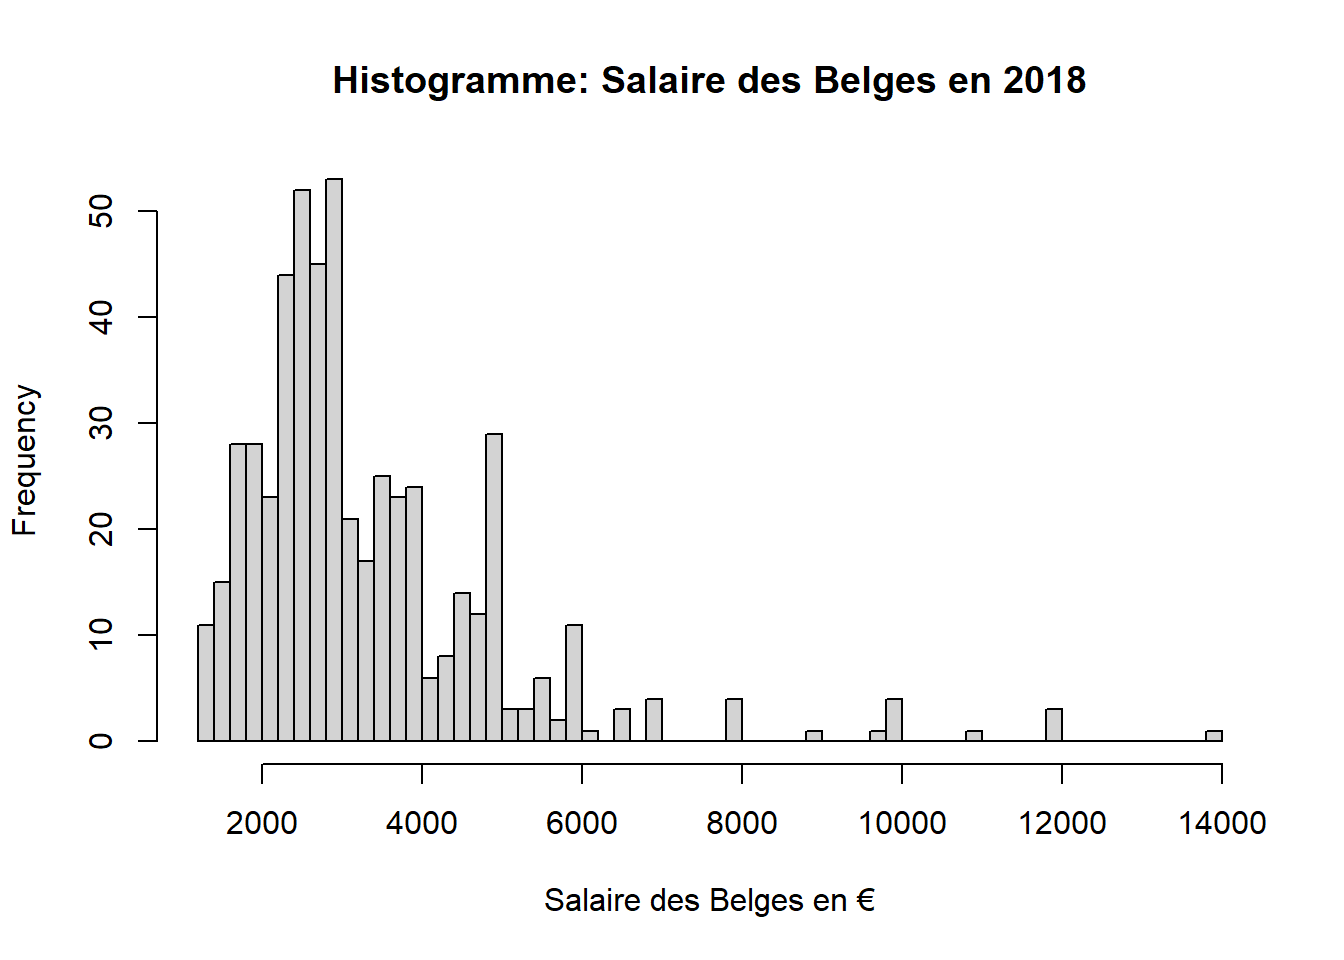
\includegraphics[width=0.5\linewidth]{bookdown-demo_files/figure-latex/unnamed-chunk-54-1} 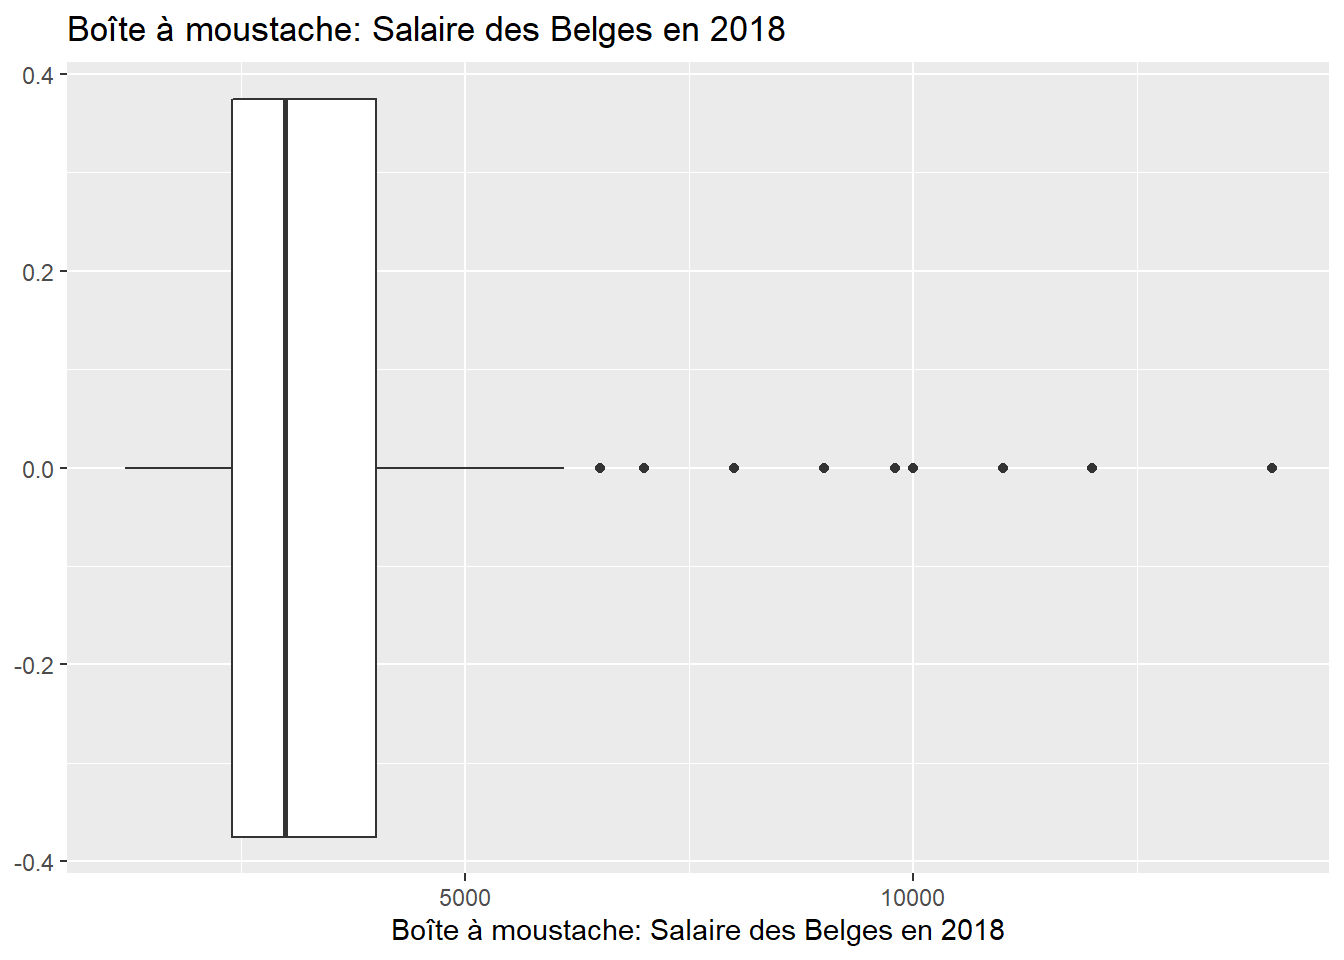
\includegraphics[width=0.5\linewidth]{bookdown-demo_files/figure-latex/unnamed-chunk-54-2}
Avec des \emph{boxplot}, la variable \emph{grspnum} donne le résultat suivant:

\begin{Shaded}
\begin{Highlighting}[]
\CommentTok{\#Avec R de base:}

\FunctionTok{boxplot}\NormalTok{(ESS9\_BE\_fulltime}\SpecialCharTok{$}\NormalTok{grspnum,}
        \AttributeTok{ylab =} \StringTok{"Salaire des Belges en €"}\NormalTok{,}
     \AttributeTok{main =} \StringTok{"Boîte à moustache: Salaire des Belges en 2018"}\NormalTok{) }

\CommentTok{\#Avec ggplot2:}

\NormalTok{ESS9\_BE\_fulltime }\SpecialCharTok{\%\textgreater{}\%} \FunctionTok{ggplot}\NormalTok{(}\FunctionTok{aes}\NormalTok{(}\AttributeTok{x=}\NormalTok{grspnum)) }\SpecialCharTok{+} 
  \FunctionTok{geom\_boxplot}\NormalTok{() }\SpecialCharTok{+} \FunctionTok{ggtitle}\NormalTok{(}\StringTok{"Boîte à moustache: Salaire des Belges en 2018"}\NormalTok{)}\SpecialCharTok{+}
  \FunctionTok{xlab}\NormalTok{(}\StringTok{"Boîte à moustache: Salaire des Belges en 2018"}\NormalTok{)}
\end{Highlighting}
\end{Shaded}

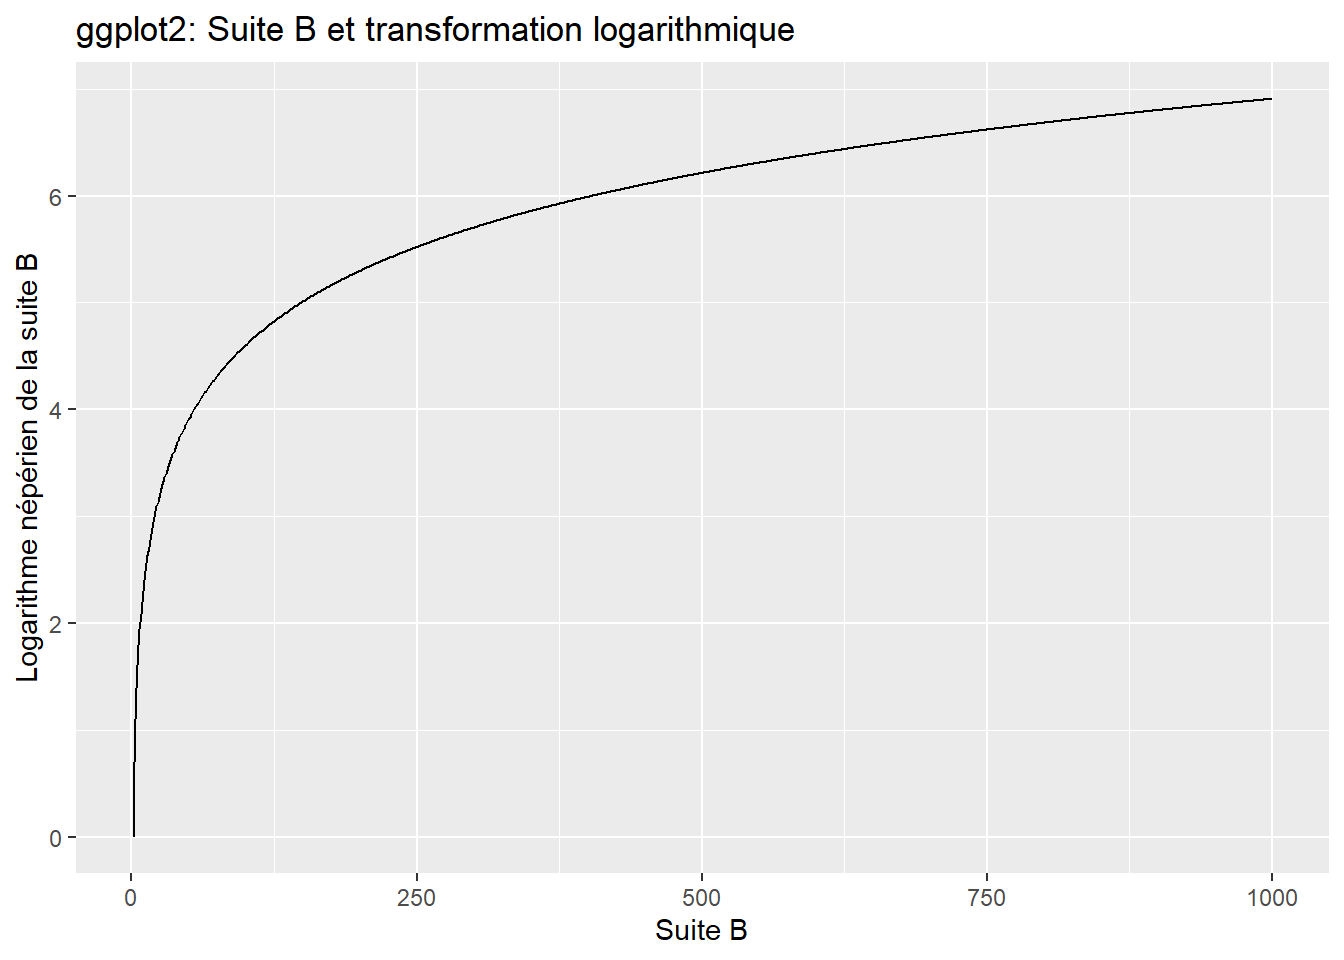
\includegraphics[width=0.5\linewidth]{bookdown-demo_files/figure-latex/unnamed-chunk-55-1} 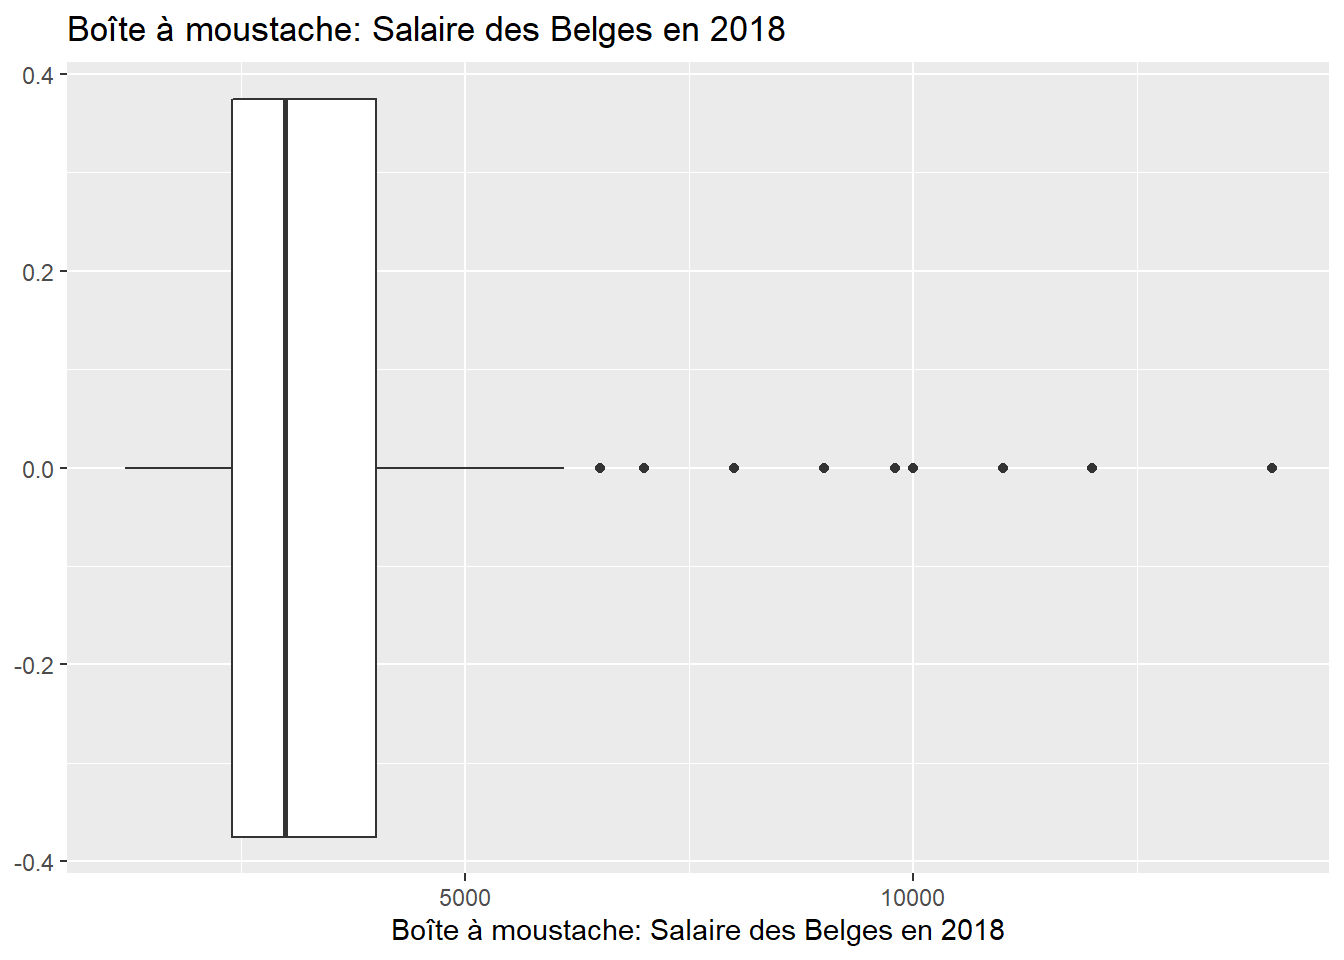
\includegraphics[width=0.5\linewidth]{bookdown-demo_files/figure-latex/unnamed-chunk-55-2}

L'histogramme et la boîte à moustache montrent une distribution moins ``écrasée''. Elle reste cependant asymétrique avec des valeurs très élevées -- et une ``coupure'' vers le bas à \(1200€\). La distribution semble donc toujours loin d'être normale.

\hypertarget{comparer-une-distribution-uxe0-une-distribution-normale}{%
\section{Comparer une distribution à une distribution normale}\label{comparer-une-distribution-uxe0-une-distribution-normale}}

Visuellement, la distribution de la variable des salaires (\emph{grspnum}) ne semble pas normale. Essayons d'objectiver cela. Nous rappelons quelques caractéristiques d'une distribution normale:

\begin{itemize}
\tightlist
\item
  la distribution est symétrique;
\item
  moyenne \(=\) médiane \(=\) mode;
\item
  \(\approx68\%\) des observations se trouvent dans l'intervalle entre \(-1\) écart type (\(\sigma\)) et \(+1\) écart type (\(\sigma\)) de la moyenne (\(\mu\)): \([\mu-\sigma;\mu+\sigma]\)
\item
  \(\approx95\%\) des observations se trouvent dans l'intervalle entre \(-1,96\) écart type (\(\sigma\)) et \(+1,96\) écart type (\(\sigma\)) de la moyenne (\(\mu\)): \([\mu-1,96\sigma;\mu+1,96\sigma]\)
\item
  \(\approx95,5\%\) des observations se trouvent dans l'intervalle entre \(-2\) écart type (\(\sigma\)) et \(+2\) écart type (\(\sigma\)) de la moyenne (\(\mu\)): \([\mu-2\sigma;\mu+2\sigma]\)
\item
  \(\approx2,5\%\) des observation sont supérieures à \(1,96\) écart type (\(\sigma\)) de la moyenne (\(\mu\)): \([\mu+1,96\sigma;+\infty)\)
\item
  \(\approx2,5\%\) des observation inférieurs à \(-1,96\) écart type (\(\sigma\)) de la moyenne (\(\mu\)): \([\mu-1,96\sigma;-\infty)\)
\end{itemize}

La fonction \emph{nonantecinq()} que nous définissions permet de comparer la distribution d'une variable avec les caractéristiques d'une distribution normale. Pour définir une nouvelle fonction, il faut utiliser la fonction \href{https://www.rdocumentation.org/packages/base/versions/3.6.2/topics/function}{\emph{fonction()}}\footnote{Vu qu'il ne s'agit pas d'une introduction à la programmation avec R, nous ne nous attardons pas sur l'écriture de fonctions dans R. Nous renvoyons à l'ouvrage \href{https://cran.r-project.org/doc/contrib/Goulet_introduction_programmation_R.pdf}{``Introduction à la programmation en R''} de Vincent Goulet et plus particulièrement au chapitre 5: ``Fonctions définies par l'usager''.}:

\begin{Shaded}
\begin{Highlighting}[]
\NormalTok{nonantecinq}\OtherTok{\textless{}{-}}\ControlFlowTok{function}\NormalTok{(x)\{}
  \CommentTok{\#On exclut les valeurs manquantes de la variable analysée}
\NormalTok{  x1}\OtherTok{\textless{}{-}}\NormalTok{x[}\FunctionTok{is.na}\NormalTok{(x)}\SpecialCharTok{!=}\NormalTok{T]}
  \CommentTok{\#On calcule l\textquotesingle{}effectif total}
\NormalTok{  x1\_l1}\OtherTok{\textless{}{-}}\FunctionTok{length}\NormalTok{(x[}\FunctionTok{is.na}\NormalTok{(x)}\SpecialCharTok{!=}\NormalTok{T])}
  \CommentTok{\#On calcule l\textquotesingle{}effectif se situant à {-}1,96 écart types de la moyenne}
\NormalTok{  x1\_low}\OtherTok{\textless{}{-}}\FunctionTok{length}\NormalTok{(x1[x1 }\SpecialCharTok{\textless{}} \FunctionTok{mean}\NormalTok{(x1, }\AttributeTok{na.rm=}\NormalTok{T)}\SpecialCharTok{{-}}\FloatTok{1.96}\SpecialCharTok{*}\FunctionTok{sd}\NormalTok{(x1, }\AttributeTok{na.rm=}\NormalTok{T)])}
  \CommentTok{\#On calcule l\textquotesingle{}effectif se situant à +1,96 écart types de la moyenne}
\NormalTok{  x1\_high}\OtherTok{\textless{}{-}}\FunctionTok{length}\NormalTok{(x1[x1 }\SpecialCharTok{\textgreater{}} \FunctionTok{mean}\NormalTok{(x1, }\AttributeTok{na.rm=}\NormalTok{T)}\SpecialCharTok{+}\FloatTok{1.96}\SpecialCharTok{*}\FunctionTok{sd}\NormalTok{(x1, }\AttributeTok{na.rm=}\NormalTok{T)])}
  \CommentTok{\#On calcule l\textquotesingle{}effectif se situant à {-}1 écarts types de la moyenne (point d\textquotesingle{}inflexion si normal)}
\NormalTok{  x1\_low\_inflex}\OtherTok{\textless{}{-}}\FunctionTok{length}\NormalTok{(x1[x1 }\SpecialCharTok{\textless{}} \FunctionTok{mean}\NormalTok{(x1, }\AttributeTok{na.rm=}\NormalTok{T)}\SpecialCharTok{{-}}\FunctionTok{sd}\NormalTok{(x1, }\AttributeTok{na.rm=}\NormalTok{T)])}
  \CommentTok{\#On calcule l\textquotesingle{}effectif se situant à +1 écart types de la moyenne (point d\textquotesingle{}inflexion si normal)}
\NormalTok{  x1\_high\_inflex}\OtherTok{\textless{}{-}}\FunctionTok{length}\NormalTok{(x1[x1 }\SpecialCharTok{\textgreater{}} \FunctionTok{mean}\NormalTok{(x1, }\AttributeTok{na.rm=}\NormalTok{T)}\SpecialCharTok{+}\FunctionTok{sd}\NormalTok{(x1, }\AttributeTok{na.rm=}\NormalTok{T)])}
  
  \CommentTok{\#Pourcentages:}
\NormalTok{  pourcent\_bas}\OtherTok{\textless{}{-}}\NormalTok{x1\_low}\SpecialCharTok{/}\NormalTok{x1\_l1}
\NormalTok{  pourcent\_haut}\OtherTok{\textless{}{-}}\NormalTok{x1\_high}\SpecialCharTok{/}\NormalTok{x1\_l1}
\NormalTok{  pourcent\_1}\FloatTok{.96}\OtherTok{\textless{}{-}}\NormalTok{(}\DecValTok{1}\SpecialCharTok{{-}}\NormalTok{(pourcent\_bas}\SpecialCharTok{+}\NormalTok{pourcent\_haut))}\SpecialCharTok{*}\DecValTok{100}
\NormalTok{  pourcent\_inflex\_bas}\OtherTok{\textless{}{-}}\NormalTok{x1\_low\_inflex}\SpecialCharTok{/}\NormalTok{x1\_l1}
\NormalTok{  pourcent\_inflex\_haut}\OtherTok{\textless{}{-}}\NormalTok{x1\_high\_inflex}\SpecialCharTok{/}\NormalTok{x1\_l1}
\NormalTok{  pourcent\_1\_inflex}\OtherTok{\textless{}{-}}\NormalTok{(}\DecValTok{1}\SpecialCharTok{{-}}\NormalTok{ (pourcent\_inflex\_bas }\SpecialCharTok{+}\NormalTok{ pourcent\_inflex\_haut))}\SpecialCharTok{*}\DecValTok{100}
  
  \CommentTok{\#Mode(s)}
\NormalTok{  mode\_func }\OtherTok{\textless{}{-}} \ControlFlowTok{function}\NormalTok{(x\_1) \{                    }
\NormalTok{    modes\_multi}\OtherTok{\textless{}{-}}\FunctionTok{which}\NormalTok{(}\FunctionTok{table}\NormalTok{(x\_1)}\SpecialCharTok{==}\FunctionTok{max}\NormalTok{(}\FunctionTok{table}\NormalTok{(x\_1)))}
\NormalTok{    mode\_final}\OtherTok{\textless{}{-}}\FunctionTok{as.numeric}\NormalTok{(}\FunctionTok{names}\NormalTok{(modes\_multi))}
    \FunctionTok{return}\NormalTok{(mode\_final)}
\NormalTok{  \}}
  
\NormalTok{  mode\_calc}\OtherTok{\textless{}{-}}\FunctionTok{mode\_func}\NormalTok{(x)}
  
  \CommentTok{\#Affichage des résultats}
  \FunctionTok{message}\NormalTok{(}\FunctionTok{paste}\NormalTok{(}\StringTok{" Moyenne="}\NormalTok{,}\FunctionTok{round}\NormalTok{(}\FunctionTok{mean}\NormalTok{(x1, }\AttributeTok{na.rm=}\NormalTok{T),}\DecValTok{2}\NormalTok{),}\StringTok{"}\SpecialCharTok{\textbackslash{}n}\StringTok{"}\NormalTok{,}
                \StringTok{"Écart type="}\NormalTok{,}\FunctionTok{round}\NormalTok{(}\FunctionTok{sd}\NormalTok{(x1, }\AttributeTok{na.rm=}\NormalTok{T),}\DecValTok{2}\NormalTok{),}\StringTok{"}\SpecialCharTok{\textbackslash{}n}\StringTok{"}\NormalTok{,}
                \StringTok{"Médiane="}\NormalTok{,}\FunctionTok{round}\NormalTok{(}\FunctionTok{median}\NormalTok{(x1, }\AttributeTok{na.rm=}\NormalTok{T),}\DecValTok{2}\NormalTok{),}\StringTok{"}\SpecialCharTok{\textbackslash{}n}\StringTok{"}\NormalTok{,}
                \StringTok{"Mode (si multiples, le plus faible)="}\NormalTok{,}\FunctionTok{ifelse}\NormalTok{(}\FunctionTok{length}\NormalTok{(mode\_calc)}\SpecialCharTok{\textgreater{}}\DecValTok{1}\NormalTok{, }\FunctionTok{round}\NormalTok{(mode\_calc[}\DecValTok{1}\NormalTok{],}\DecValTok{2}\NormalTok{), }\FunctionTok{round}\NormalTok{(mode\_calc,}\DecValTok{2}\NormalTok{)),}\StringTok{"}\SpecialCharTok{\textbackslash{}n}\StringTok{"}\NormalTok{,}
                \StringTok{"Le point d\textquotesingle{}inflexion (si la distribution est normale) à {-}1 écart type prend la valeur:"}\NormalTok{, }\FunctionTok{round}\NormalTok{(}\FunctionTok{mean}\NormalTok{(x1, }\AttributeTok{na.rm=}\NormalTok{T)}\SpecialCharTok{{-}}\FunctionTok{sd}\NormalTok{(x1, }\AttributeTok{na.rm=}\NormalTok{T),}\DecValTok{2}\NormalTok{),}\StringTok{"}\SpecialCharTok{\textbackslash{}n}\StringTok{"}\NormalTok{,}
                \StringTok{"Le point d\textquotesingle{}inflexion (si la distribution est normale) à +1 écart type prend la valeur:"}\NormalTok{, }\FunctionTok{round}\NormalTok{(}\FunctionTok{mean}\NormalTok{(x1, }\AttributeTok{na.rm=}\NormalTok{T)}\SpecialCharTok{+}\FunctionTok{sd}\NormalTok{(x1, }\AttributeTok{na.rm=}\NormalTok{T),}\DecValTok{2}\NormalTok{),}\StringTok{"}\SpecialCharTok{\textbackslash{}n}\StringTok{"}\NormalTok{,}
                \FunctionTok{round}\NormalTok{(pourcent\_1\_inflex,}\DecValTok{2}\NormalTok{),}\StringTok{"\%"}\NormalTok{,}\StringTok{" des valeurs se situent entre {-}1 et +1 écart types de la moyenne."}\NormalTok{, }\StringTok{"}\SpecialCharTok{\textbackslash{}n}\StringTok{"}\NormalTok{,}
                \FunctionTok{round}\NormalTok{(pourcent\_inflex\_bas}\SpecialCharTok{*}\DecValTok{100}\NormalTok{,}\DecValTok{2}\NormalTok{),}\StringTok{"\%"}\NormalTok{,}\StringTok{" des valeurs se situent en dessous de {-}1 écart types de la moyenne."}\NormalTok{,}\StringTok{"}\SpecialCharTok{\textbackslash{}n}\StringTok{"}\NormalTok{,}
                \FunctionTok{round}\NormalTok{(pourcent\_inflex\_haut}\SpecialCharTok{*}\DecValTok{100}\NormalTok{,}\DecValTok{2}\NormalTok{),}\StringTok{"\%"}\NormalTok{,}\StringTok{" des valeurs se situent au{-}dessus de 1 écart types de la moyenne."}\NormalTok{,}\StringTok{"}\SpecialCharTok{\textbackslash{}n}\StringTok{"}\NormalTok{,}
                \StringTok{"{-}1,96 écarts types prend la valeur:"}\NormalTok{, }\FunctionTok{round}\NormalTok{(}\FunctionTok{mean}\NormalTok{(x1, }\AttributeTok{na.rm=}\NormalTok{T)}\SpecialCharTok{{-}}\FloatTok{1.96}\SpecialCharTok{*}\FunctionTok{sd}\NormalTok{(x1, }\AttributeTok{na.rm=}\NormalTok{T),}\DecValTok{2}\NormalTok{), }\StringTok{"}\SpecialCharTok{\textbackslash{}n}\StringTok{"}\NormalTok{,}
                \StringTok{"+1,96 écarts types prend la valeur:"}\NormalTok{, }\FunctionTok{round}\NormalTok{(}\FunctionTok{mean}\NormalTok{(x1, }\AttributeTok{na.rm=}\NormalTok{T)}\SpecialCharTok{+}\FloatTok{1.96}\SpecialCharTok{*}\FunctionTok{sd}\NormalTok{(x1, }\AttributeTok{na.rm=}\NormalTok{T),}\DecValTok{2}\NormalTok{), }\StringTok{"}\SpecialCharTok{\textbackslash{}n}\StringTok{"}\NormalTok{,}
                \FunctionTok{round}\NormalTok{(pourcent\_1}\FloatTok{.96}\NormalTok{,}\DecValTok{2}\NormalTok{),}\StringTok{"\%"}\NormalTok{, }\StringTok{" des valeurs se situent entre {-}1,96 et +1,96 écart types de la moyenne."}\NormalTok{, }\StringTok{"}\SpecialCharTok{\textbackslash{}n}\StringTok{"}\NormalTok{,}
                \FunctionTok{round}\NormalTok{(pourcent\_bas}\SpecialCharTok{*}\DecValTok{100}\NormalTok{,}\DecValTok{2}\NormalTok{),}\StringTok{"\%"}\NormalTok{,}\StringTok{" des valeurs se situent en dessous de {-}1,96 écart types de la moyenne."}\NormalTok{,}\StringTok{"}\SpecialCharTok{\textbackslash{}n}\StringTok{"}\NormalTok{,}
                \FunctionTok{round}\NormalTok{(pourcent\_haut}\SpecialCharTok{*}\DecValTok{100}\NormalTok{,}\DecValTok{2}\NormalTok{),}\StringTok{"\%"}\NormalTok{, }\StringTok{" des valeurs se situent au{-}dessus de 1,96 écart types de la moyenne."}\NormalTok{)}
\NormalTok{  )}
\NormalTok{\}}
\end{Highlighting}
\end{Shaded}

Une fois que vous avez exécuté le code ci-dessus, la fonction \emph{nonantecinq()} apparaîtra dans l'\protect\hyperlink{objets_envir}{environnement global} de R. Si vous fermer R et que vous n'enregistrez pas cet \protect\hyperlink{objets_envir}{environnement global}, vous devrez récréer la fonction \emph{nonantecinq()} avec le code ci-dessus. Lorsque la fonction \emph{nonantecinq()} est définie, vous pouvez la lancer comme toutes les fonctions de R de base ou des \emph{packages}. Vous indiquez simplement le nom de la fonction avec les parenthèses dans lesquelles vous ajoutez, le cas échéant le ou les arguments. La fonction \emph{nonantecinq()} ne prend qu'un seul argument qui doit être un vecteur numérique (une variable contenant des nombres). Ici, nous voulons vérifier le salaire des Belges (\emph{grspnum}):

\begin{Shaded}
\begin{Highlighting}[]
\FunctionTok{nonantecinq}\NormalTok{(ESS9\_BE\_fulltime}\SpecialCharTok{$}\NormalTok{grspnum)}
\end{Highlighting}
\end{Shaded}

\begin{verbatim}
##  Moyenne= 3365.44 
##  Écart type= 1673.51 
##  Médiane= 2986 
##  Mode (si multiples, le plus faible)= 3000 
##  Le point d'inflexion (si la distribution est normale) à -1 écart type prend la valeur: 1691.93 
##  Le point d'inflexion (si la distribution est normale) à +1 écart type prend la valeur: 5038.96 
##  85.36 %  des valeurs se situent entre -1 et +1 écart types de la moyenne. 
##  5.51 %  des valeurs se situent en dessous de -1 écart types de la moyenne. 
##  9.13 %  des valeurs se situent au-dessus de 1 écart types de la moyenne. 
##  -1,96 écarts types prend la valeur: 85.35 
##  +1,96 écarts types prend la valeur: 6645.53 
##  96.39 %  des valeurs se situent entre -1,96 et +1,96 écart types de la moyenne. 
##  0 %  des valeurs se situent en dessous de -1,96 écart types de la moyenne. 
##  3.61 %  des valeurs se situent au-dessus de 1,96 écart types de la moyenne.
\end{verbatim}

On voit donc également de manière ``objective'' que la variable salaire (\emph{grspnum}) n'est absolument pas normale:

\begin{itemize}
\tightlist
\item
  La distribution n'est pas symétrique: \(5,51\%\) des valeurs se situent en dessous de -1 écart types de la moyenne, tandis que \(9,13\%\) des valeurs se situent au-dessus de 1 écart types de la moyenne.
\item
  La moyenne, la médiane et le mode sont différents. En particulier, la moyenne est plus élevée que le mode et la médiane.
\item
  \(\approx85\%\) des observations se trouvent entre -1 et +1 écart type (contre \(68\%\) pour une distribution normale)
\item
  \(0\%\) des observations se trouvent en dessous de \(1,96\) écart types (contre \(2,5\%\) pour une distribution normale)
\item
  \(3,6\%\) des observations se trouvent au-dessus de \(1,96\) écart types (contre \(2,5\%\) pour une distribution normale)
\end{itemize}

\hypertarget{trans_log_grspnum}{%
\section{Distribution normale et transformation logarithmique}\label{trans_log_grspnum}}

La distribution de la variable des salaires (\emph{grspnum}) est très éloignée d'une distribution normale. Quelques observations très élevées ``tirent'' la moyenne vers le haut. Cela est habituel pour les variables de type salaire ou patrimoine. Cependant, l'on peut souvent transformer ces variables de manière à les rapprocher d'une distribution normale. Une transformation très usitée pour cela est la transformation logarithmique (on prend souvent le \href{https://fr.wikipedia.org/wiki/Logarithme_naturel}{logarithme népérien}). Cela a pour effet de davantage espacer les valeurs faibles tout en réduisant les espaces entre les valeurs élevées. Nous vous illustrons cela graphiquement à l'aide une suite \(B\) allant de \(1\) à \(1000\):

\begin{Shaded}
\begin{Highlighting}[]
\NormalTok{suite\_B}\OtherTok{\textless{}{-}}\DecValTok{1}\SpecialCharTok{:}\DecValTok{1000} \CommentTok{\# Créons vecteur de 1 à 1000}
\NormalTok{log\_suite\_B}\OtherTok{\textless{}{-}}\FunctionTok{log}\NormalTok{(suite\_B) }\CommentTok{\# Vecteur du logarithme de la suite B}
\NormalTok{suite\_B\_matrix}\OtherTok{\textless{}{-}}\FunctionTok{cbind}\NormalTok{(suite\_B,log\_suite\_B) }\CommentTok{\# Nous créons une matrice avec les deux vecteurs}
\NormalTok{suite\_B\_df}\OtherTok{\textless{}{-}}\FunctionTok{as.data.frame}\NormalTok{(suite\_B\_matrix) }\CommentTok{\# Nous la transformons en base de données (dataframe)}
\NormalTok{suite\_B\_df }\SpecialCharTok{\%\textgreater{}\%} \CommentTok{\# nous utilisions une "pipe"}
  \FunctionTok{ggplot}\NormalTok{(}\FunctionTok{aes}\NormalTok{(}\AttributeTok{x=}\NormalTok{suite\_B,}\AttributeTok{y=}\NormalTok{log\_suite\_B)) }\SpecialCharTok{+}
  \FunctionTok{geom\_line}\NormalTok{() }\SpecialCharTok{+} \FunctionTok{xlab}\NormalTok{(}\StringTok{"Suite B"}\NormalTok{) }\SpecialCharTok{+}
  \FunctionTok{ylab}\NormalTok{(}\StringTok{"Logarithme népérien de la suite B"}\NormalTok{) }\SpecialCharTok{+}
  \FunctionTok{ggtitle}\NormalTok{(}\StringTok{"ggplot2: Suite B et transformation logarithmique"}\NormalTok{)}

\FunctionTok{plot}\NormalTok{(suite\_B\_df}\SpecialCharTok{$}\NormalTok{suite\_B, suite\_B\_df}\SpecialCharTok{$}\NormalTok{log\_suite\_B, }\AttributeTok{type =} \StringTok{"l"}\NormalTok{,}
     \AttributeTok{main=}\StringTok{"Base R: Suite B et transformation logarithmique"}\NormalTok{,}
     \AttributeTok{xlab =} \StringTok{"Suite B"}\NormalTok{,}
     \AttributeTok{ylab=}\StringTok{"Logarithme népérien de la suite B"}\NormalTok{)}
\end{Highlighting}
\end{Shaded}

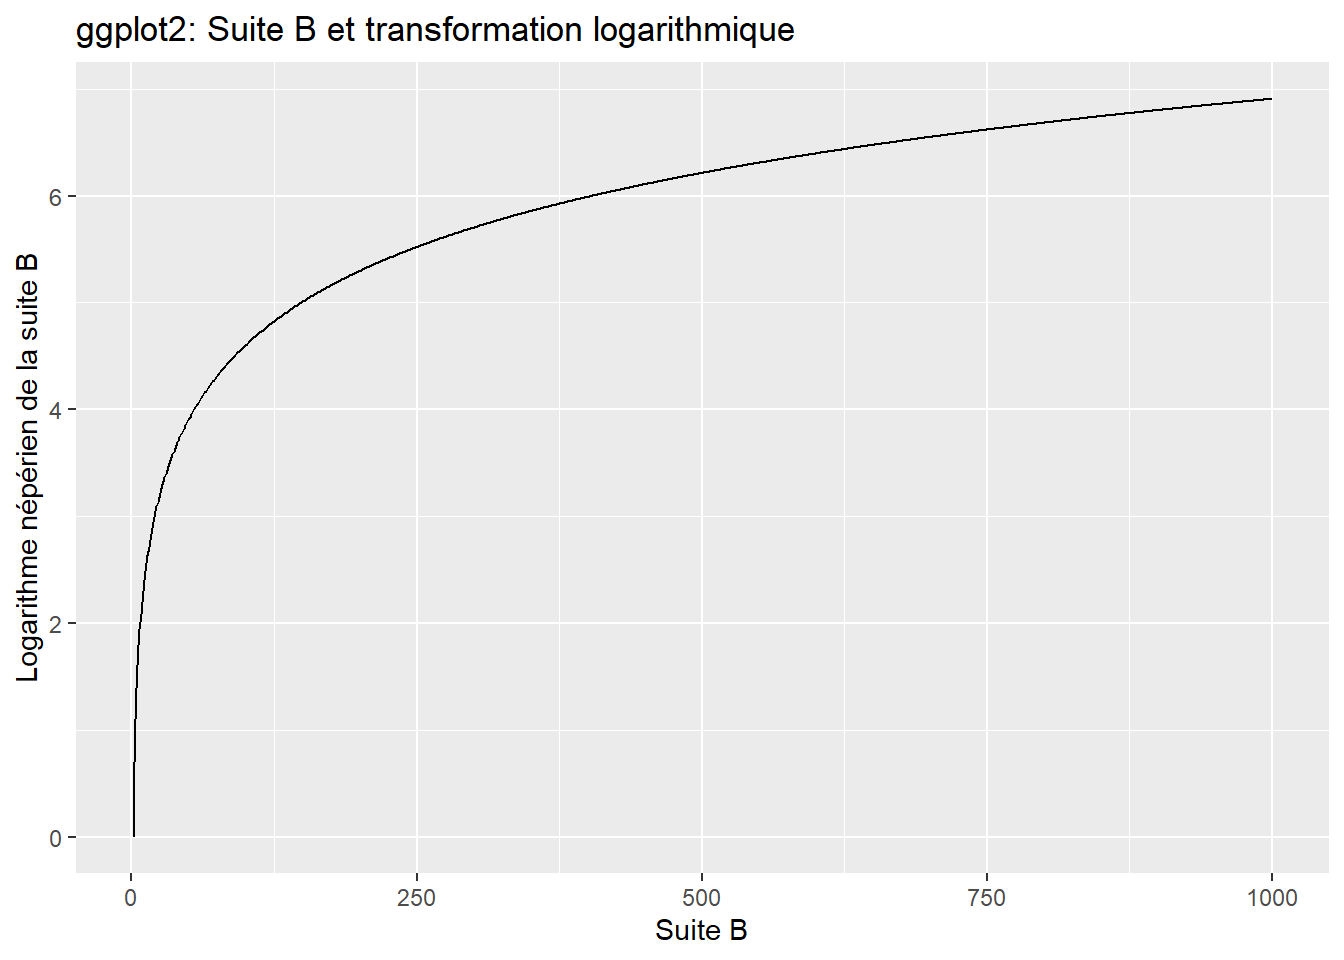
\includegraphics[width=0.5\linewidth]{bookdown-demo_files/figure-latex/unnamed-chunk-58-1} 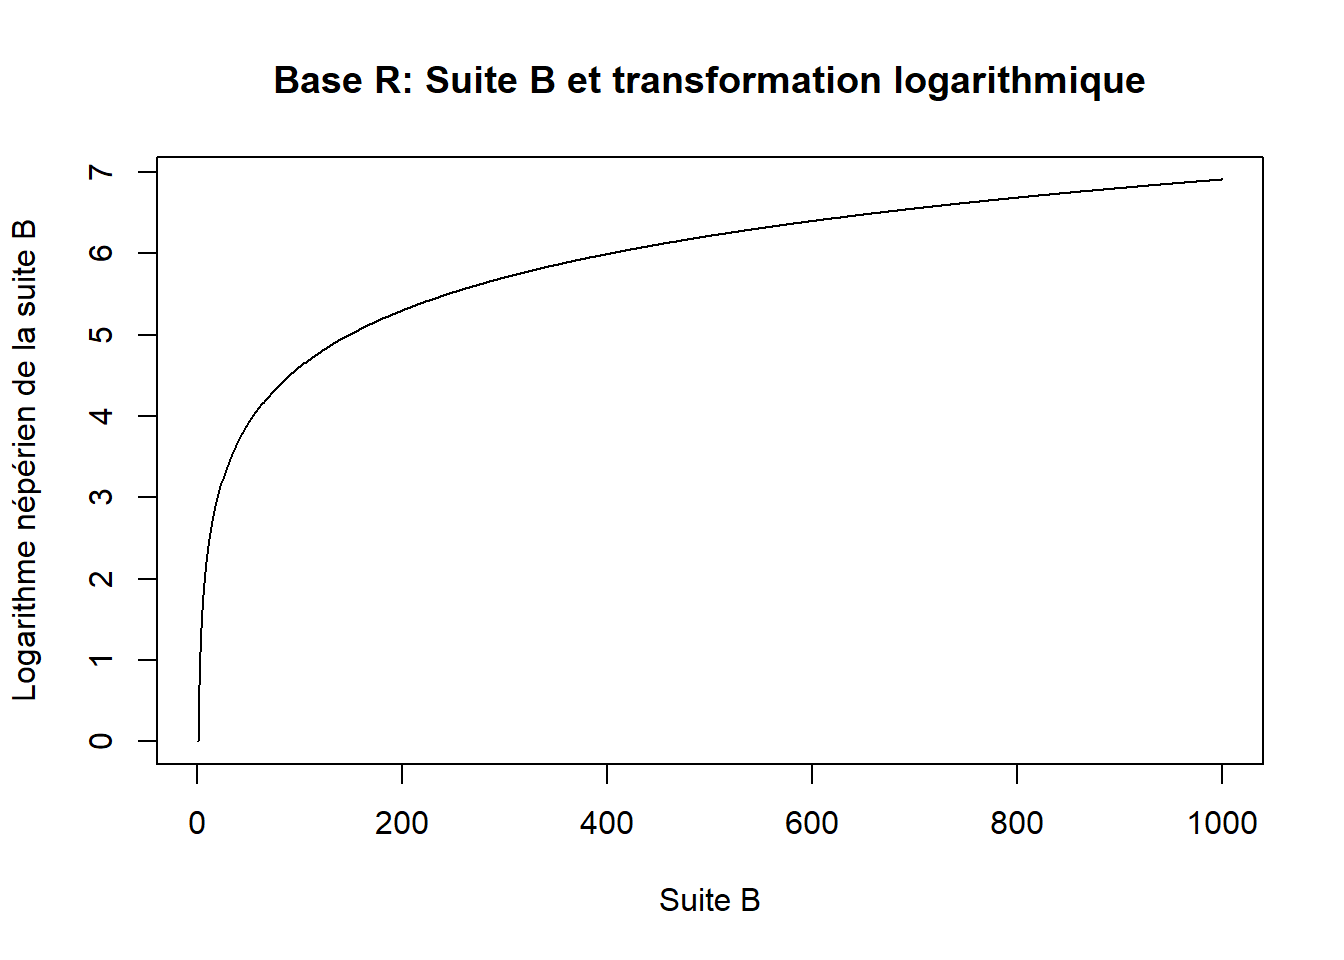
\includegraphics[width=0.5\linewidth]{bookdown-demo_files/figure-latex/unnamed-chunk-58-2}

En abscisse, l'on voit la suite \(B\) (l'objet \emph{suite\_B}) allant de 1 à 1000. En ordonné, nous avons cette même suite \(B\) transformée de manière logarithmique. L'on voit, très clairement que la courbe augmente fortement lors de faibles valeurs puis s'aplanit. Cela correspond à l'augmentation de l'espacement des valeurs faibles et au rapprochement des grandes valeurs.

Nous allons donc appliquer cette transformation à la variable \emph{grspnum} reprenant les salaires. Pour effectuer cette transformation, nous utilisons la fonction \href{https://dplyr.tidyverse.org/reference/mutate.html}{\emph{mutate()}} du \emph{package} \href{https://dplyr.tidyverse.org/}{\emph{dplyr}}: celle-ci permet de créer de nouvelles variables dans une base de données. Cette fonction s'utilise de la manière suivante: vous indiquez comme premier argument, la base de donnés dans laquelle vous souhaitez ajouter une variable. Le deuxième argument correspond au nom de cette nouvelle variable suivie du signe \(=\) et de la/des valeur(s) que doit prendre cette nouvelle variable. L'on peut ainsi indiquer que cette nouvelle variable doit correspondre au \emph{logarithme népérien} de la variable \emph{grspnum}. Le logarithme népérien se calcule avec la fonction \href{https://www.rdocumentation.org/packages/base/versions/3.6.2/topics/log}{\emph{log()}}:

\begin{Shaded}
\begin{Highlighting}[]
\NormalTok{ESS9\_BE\_fulltime }\OtherTok{\textless{}{-}} \FunctionTok{mutate}\NormalTok{(ESS9\_BE\_fulltime,}\AttributeTok{log\_grspnum=}\FunctionTok{log}\NormalTok{(grspnum))}
\end{Highlighting}
\end{Shaded}

Regardons, dans quelle mesure la distribution a changée et si l'on s'est rapproché d'une distribution normale. Vérifions à l'aide d'un histogramme et d'un \emph{boxplot} :

\begin{Shaded}
\begin{Highlighting}[]
\CommentTok{\#Avec R de base:}

\FunctionTok{hist}\NormalTok{(ESS9\_BE\_fulltime}\SpecialCharTok{$}\NormalTok{log\_grspnum,}
     \AttributeTok{breaks =} \DecValTok{30}\NormalTok{,}
   \AttributeTok{xlab =} \StringTok{"Logarithme du salaire des Belges"}\NormalTok{, }\CommentTok{\# Libellé de l\textquotesingle{}abscisse.}
     \AttributeTok{main =} \StringTok{"Histogramme: Logarithme du salaire des Belges en 2018"}\NormalTok{) }\CommentTok{\# Titre du graphique}

\CommentTok{\#Avec ggplot2:}

\NormalTok{ESS9\_BE\_fulltime }\SpecialCharTok{\%\textgreater{}\%} \FunctionTok{ggplot}\NormalTok{(}\FunctionTok{aes}\NormalTok{(}\AttributeTok{x=}\NormalTok{log\_grspnum)) }\SpecialCharTok{+} 
  \FunctionTok{geom\_histogram}\NormalTok{(}\AttributeTok{bins =} \DecValTok{30}\NormalTok{) }\SpecialCharTok{+}
  \FunctionTok{ggtitle}\NormalTok{(}\StringTok{"Histogramme: Logarithme du salaire des Belges en 2018"}\NormalTok{) }\SpecialCharTok{+}
  \FunctionTok{xlab}\NormalTok{(}\StringTok{"Logarithme du salaire des Belges"}\NormalTok{)}
\end{Highlighting}
\end{Shaded}

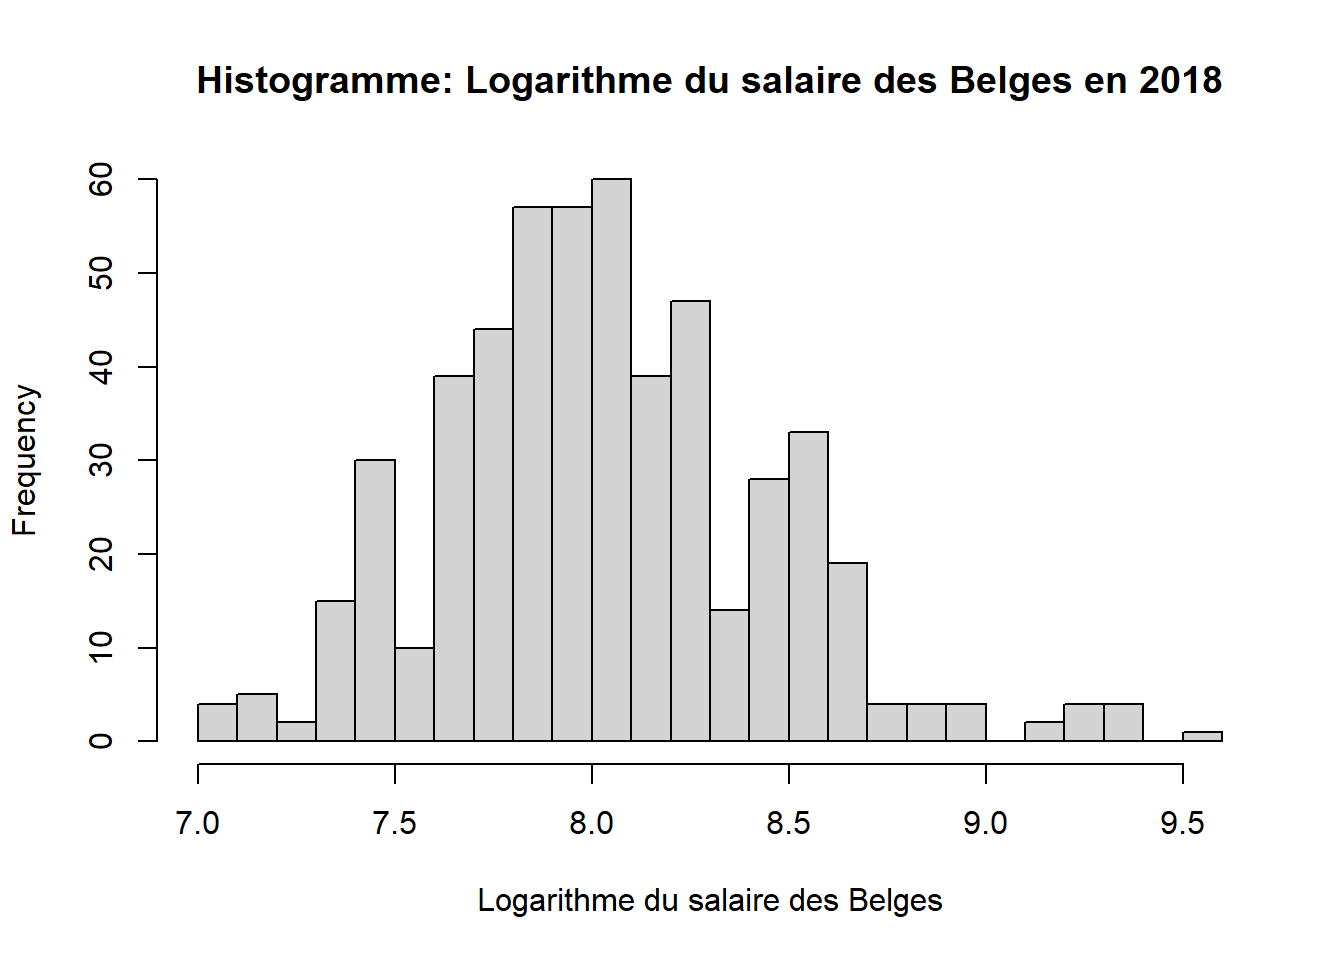
\includegraphics[width=0.5\linewidth]{bookdown-demo_files/figure-latex/unnamed-chunk-60-1} 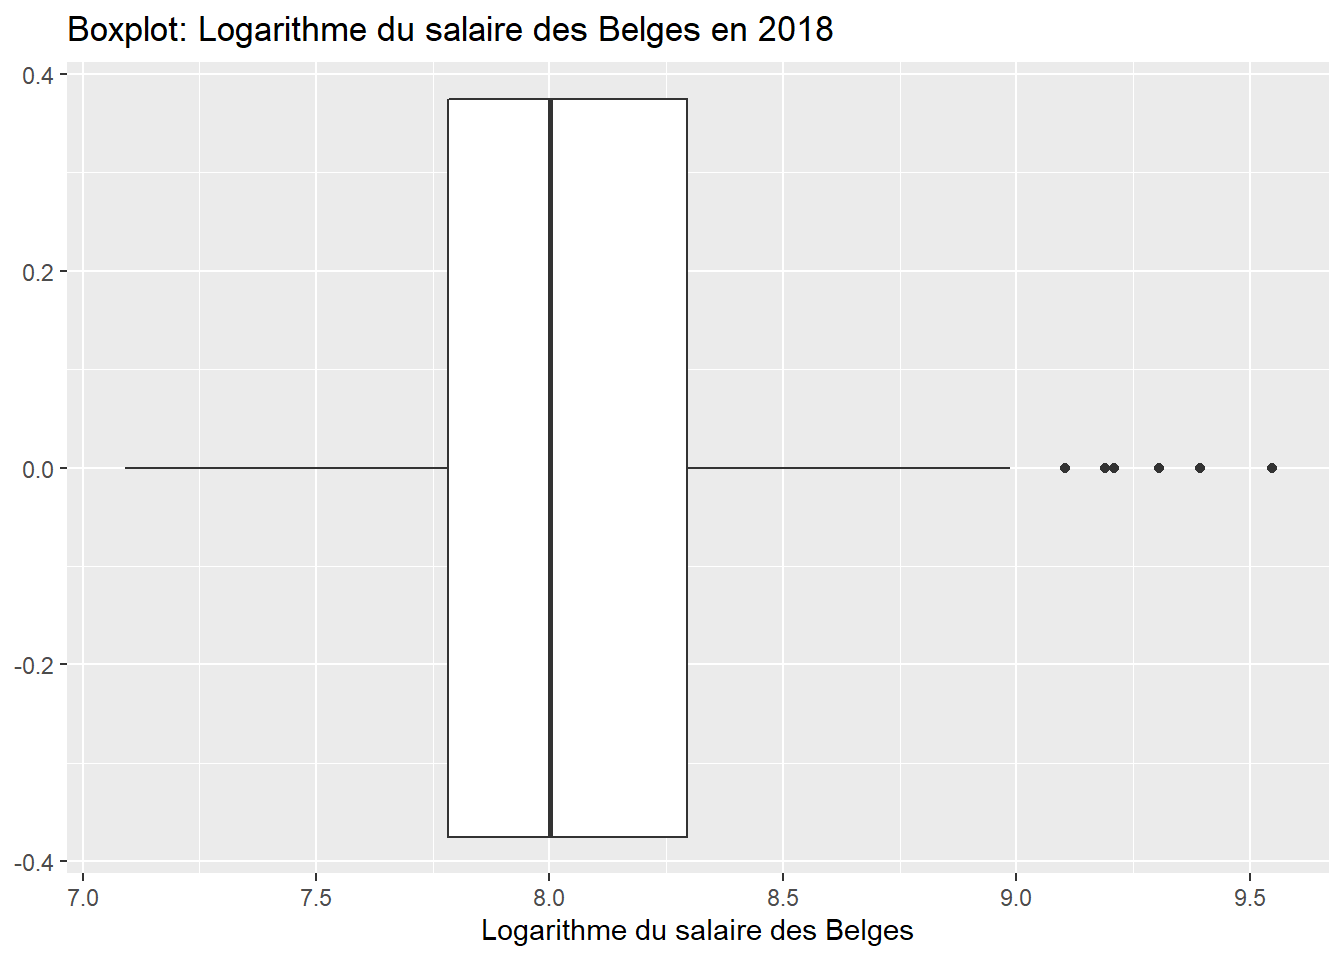
\includegraphics[width=0.5\linewidth]{bookdown-demo_files/figure-latex/unnamed-chunk-60-2}

\begin{Shaded}
\begin{Highlighting}[]
\CommentTok{\#Avec R de base:}

\FunctionTok{boxplot}\NormalTok{(ESS9\_BE\_fulltime}\SpecialCharTok{$}\NormalTok{log\_grspnum,}
   \AttributeTok{xlab =} \StringTok{"Logarithme du salaire des Belges"}\NormalTok{, }\CommentTok{\# Libellé de l\textquotesingle{}abscisse.}
     \AttributeTok{main =} \StringTok{"Histogramme: Logarithme du salaire des Belges en 2018"}\NormalTok{) }\CommentTok{\# Titre du graphique}

\CommentTok{\#Avec ggplot2:}

\NormalTok{ESS9\_BE\_fulltime }\SpecialCharTok{\%\textgreater{}\%} \FunctionTok{ggplot}\NormalTok{(}\FunctionTok{aes}\NormalTok{(}\AttributeTok{x=}\NormalTok{log\_grspnum)) }\SpecialCharTok{+} 
  \FunctionTok{geom\_boxplot}\NormalTok{() }\SpecialCharTok{+}
  \FunctionTok{ggtitle}\NormalTok{(}\StringTok{"Boxplot: Logarithme du salaire des Belges en 2018"}\NormalTok{) }\SpecialCharTok{+}
  \FunctionTok{xlab}\NormalTok{(}\StringTok{"Logarithme du salaire des Belges"}\NormalTok{)}
\end{Highlighting}
\end{Shaded}

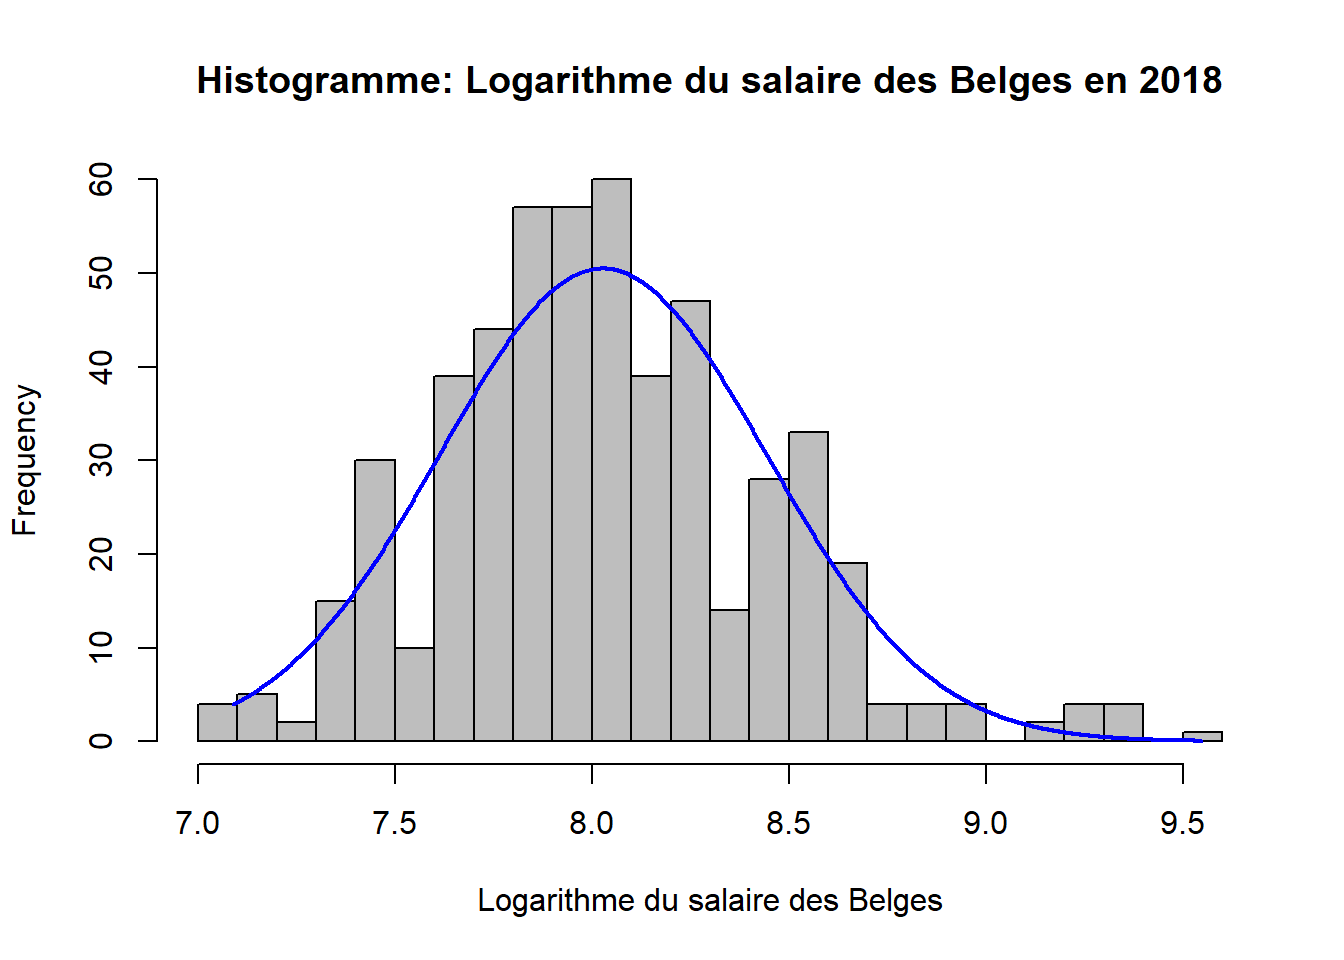
\includegraphics[width=0.5\linewidth]{bookdown-demo_files/figure-latex/unnamed-chunk-61-1} 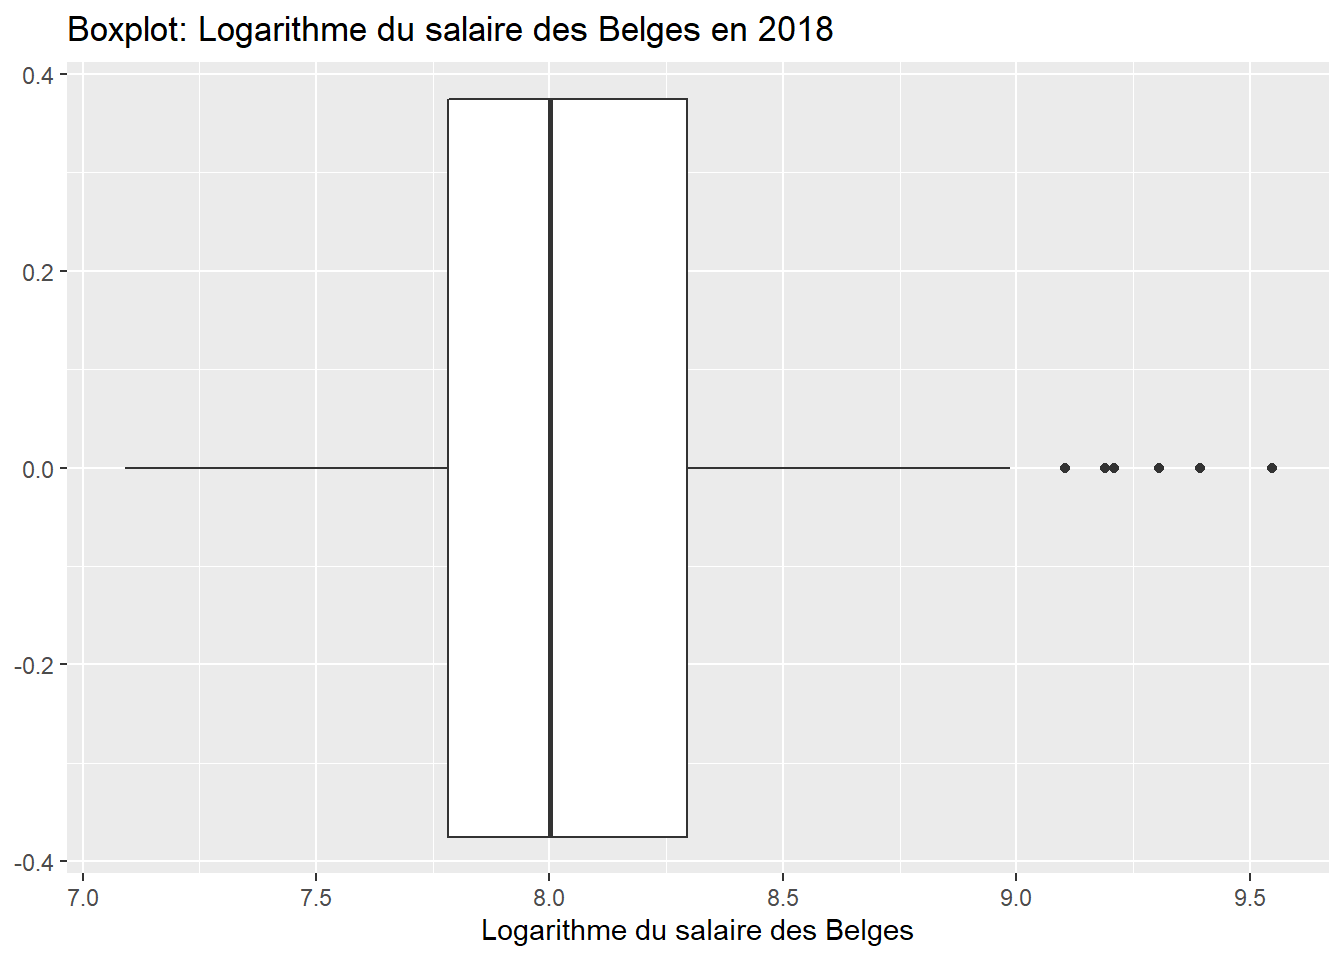
\includegraphics[width=0.5\linewidth]{bookdown-demo_files/figure-latex/unnamed-chunk-61-2}

La distribution est sensiblement moins étirée. Cela ressemble plus à une distribution normale. Comparons l'histogramme avec une courbe de densité d'une distribution normale:

\begin{Shaded}
\begin{Highlighting}[]
\CommentTok{\#Avec R de base:}

\FunctionTok{plotNormalHistogram}\NormalTok{(ESS9\_BE\_fulltime}\SpecialCharTok{$}\NormalTok{log\_grspnum,}
     \AttributeTok{breaks =} \DecValTok{30}\NormalTok{,}
   \AttributeTok{xlab =} \StringTok{"Logarithme du salaire des Belges"}\NormalTok{, }\CommentTok{\# Libellé de l\textquotesingle{}abscisse.}
     \AttributeTok{main =} \StringTok{"Histogramme: Logarithme du salaire des Belges en 2018"}\NormalTok{) }\CommentTok{\# Titre du graphique}

\CommentTok{\#Avec ggplot2:}

\NormalTok{ESS9\_BE\_fulltime }\SpecialCharTok{\%\textgreater{}\%} \FunctionTok{ggplot}\NormalTok{(}\FunctionTok{aes}\NormalTok{(}\AttributeTok{x=}\NormalTok{log\_grspnum)) }\SpecialCharTok{+} 
  \FunctionTok{geom\_histogram}\NormalTok{(}\FunctionTok{aes}\NormalTok{(}\AttributeTok{y =}\NormalTok{..density..), }\AttributeTok{bins =} \DecValTok{30}\NormalTok{) }\SpecialCharTok{+}
  \FunctionTok{stat\_function}\NormalTok{(}\AttributeTok{fun =}\NormalTok{ dnorm,}
                \AttributeTok{args =} \FunctionTok{list}\NormalTok{(}\AttributeTok{mean =} \FunctionTok{mean}\NormalTok{(ESS9\_BE\_fulltime}\SpecialCharTok{$}\NormalTok{log\_grspnum),}
                \AttributeTok{sd =} \FunctionTok{sd}\NormalTok{(ESS9\_BE\_fulltime}\SpecialCharTok{$}\NormalTok{log\_grspnum)),}
                \AttributeTok{col=}\StringTok{"blue"}\NormalTok{, }\AttributeTok{size=}\FloatTok{1.25}\NormalTok{) }\SpecialCharTok{+}
  \FunctionTok{ggtitle}\NormalTok{(}\StringTok{"Histogramme: Logarithme du salaire des Belges en 2018"}\NormalTok{) }\SpecialCharTok{+}
  \FunctionTok{xlab}\NormalTok{(}\StringTok{"Logarithme du salaire des Belges"}\NormalTok{)}
\end{Highlighting}
\end{Shaded}

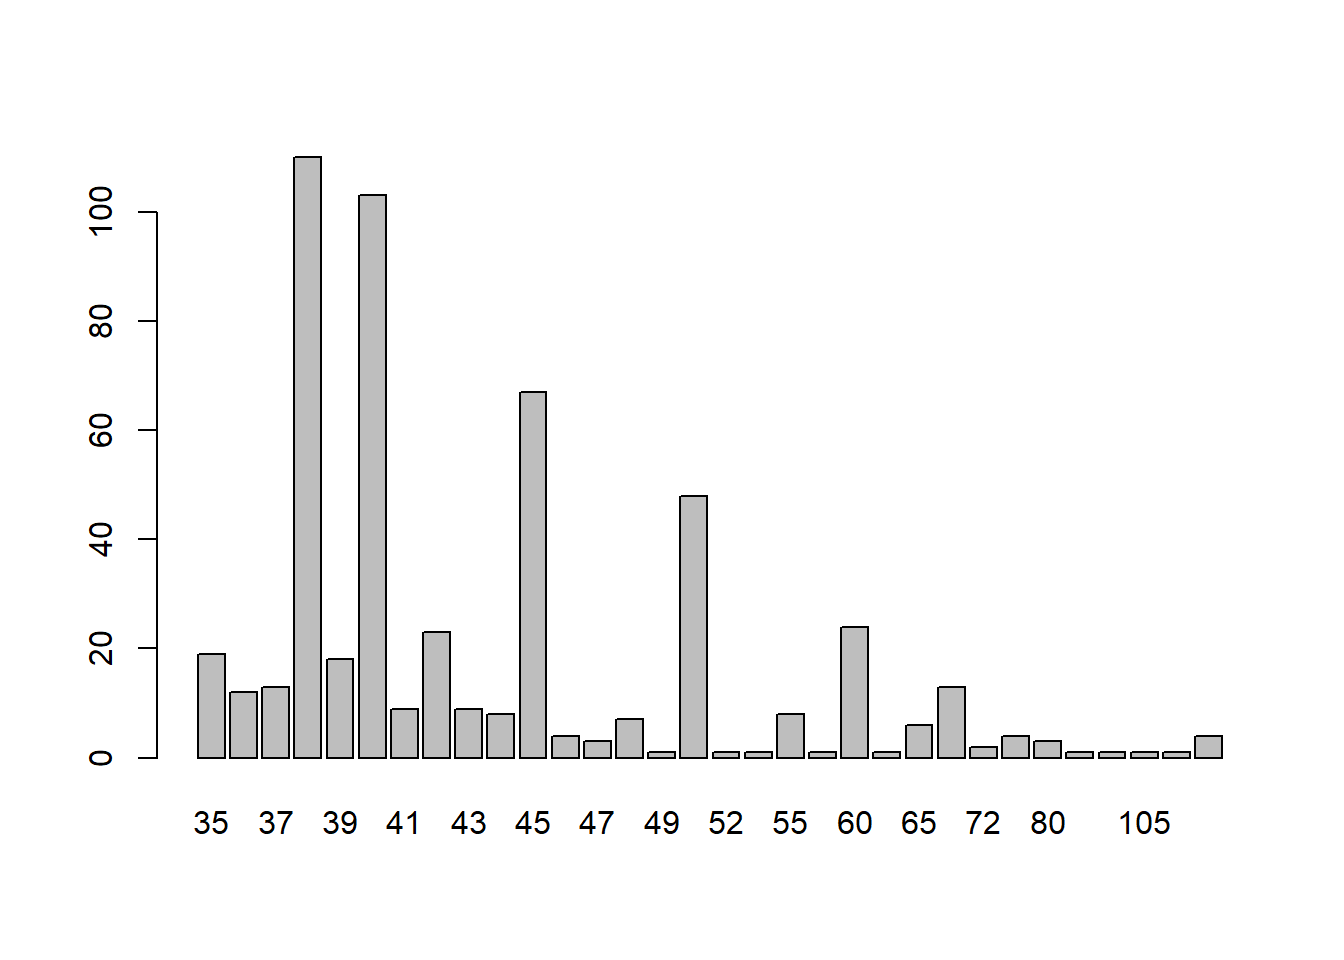
\includegraphics[width=0.5\linewidth]{bookdown-demo_files/figure-latex/unnamed-chunk-62-1} 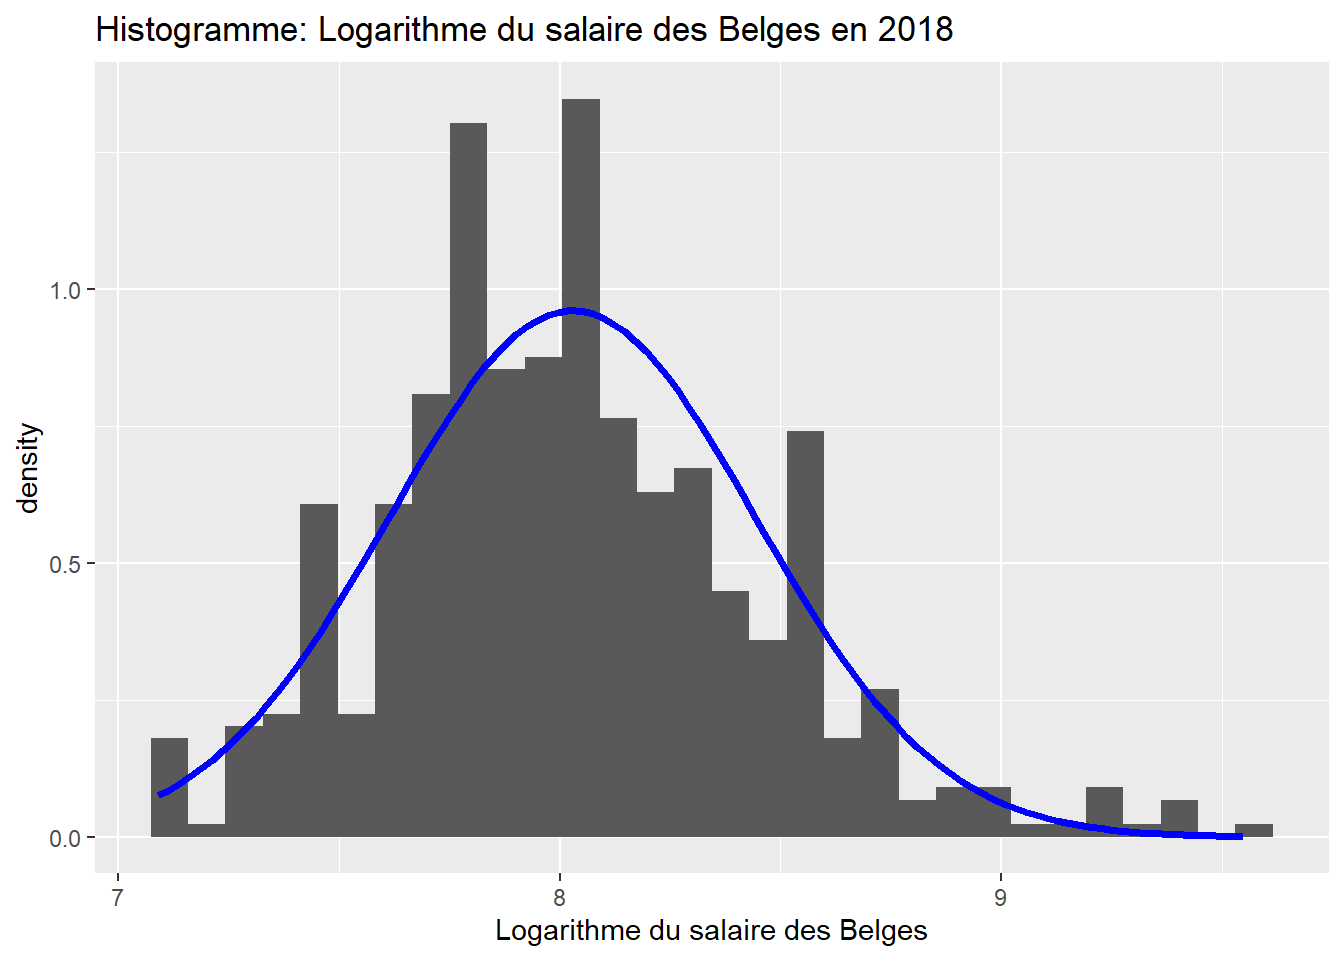
\includegraphics[width=0.5\linewidth]{bookdown-demo_files/figure-latex/unnamed-chunk-62-2}

Vérifions cela à l'aide de la fonction \emph{nonantecinq}:

\begin{Shaded}
\begin{Highlighting}[]
\FunctionTok{nonantecinq}\NormalTok{(ESS9\_BE\_fulltime}\SpecialCharTok{$}\NormalTok{log\_grspnum)}
\end{Highlighting}
\end{Shaded}

\begin{verbatim}
##  Moyenne= 8.03 
##  Écart type= 0.42 
##  Médiane= 8 
##  Mode (si multiples, le plus faible)= 8.01 
##  Le point d'inflexion (si la distribution est normale) à -1 écart type prend la valeur: 7.61 
##  Le point d'inflexion (si la distribution est normale) à +1 écart type prend la valeur: 8.44 
##  67.3 %  des valeurs se situent entre -1 et +1 écart types de la moyenne. 
##  15.78 %  des valeurs se situent en dessous de -1 écart types de la moyenne. 
##  16.92 %  des valeurs se situent au-dessus de 1 écart types de la moyenne. 
##  -1,96 écarts types prend la valeur: 7.21 
##  +1,96 écarts types prend la valeur: 8.84 
##  94.68 %  des valeurs se situent entre -1,96 et +1,96 écart types de la moyenne. 
##  1.71 %  des valeurs se situent en dessous de -1,96 écart types de la moyenne. 
##  3.61 %  des valeurs se situent au-dessus de 1,96 écart types de la moyenne.
\end{verbatim}

Les données numériques sont tout autant instructives que le diagnostic visuel:

\begin{itemize}
\tightlist
\item
  Le mode, la médiane et la moyenne sont tous très proches de \(8\) (et donc presque identiques).
\item
  \(67\%\) des observations se trouvent entre \(-1\) et \(+1\) écart type (contre \(\approx68\%\) d'une distribution normale).
\item
  \(\approx95\%\) des observations se trouvent entre \(-1,96\) et \(+1,96\) écart types (comme pour une distribution normale).
\item
  \(2\%\) des observations se trouvent en dessous de \(-1,96\) écart types et \(4%
  \) se trouvent au-dessus de \(+1,96\) écart types (contre \(2,5\%\) en dessous et au-dessus dans une distribution normale).
\end{itemize}

Empiriquement, nous ne sommes pas face à une distribution tout à fait normale, mais nous en sommes très proches. Cela d'autant plus que le salaire (\emph{grspnum}, d'où \emph{log\_grspnum}) est une variable continue, que la réponse est une déclaration spontanée (les sondés auront tendance à donner des chiffres ``ronds'')\footnote{Si l'on avait accès aux données de revenus comme l'a l'administration fiscale (en Belgique: \href{https://finances.belgium.be/fr}{SPF Finances}) et les organismes de la sécurité sociale (en Belgique notamment par le biais de la \href{https://www.ksz-bcss.fgov.be/fr}{BCSS}), la distribution serait vraisemblablement encore plus proche de la distribution normale.} et que l'échantillon est assez grand (\(n=526\)). Il y a donc une très forte probabilité que la variable sous-jacente dans la population suive une distribution normale. L'on peut donc traiter la variable salaire transformée (\emph{log\_grspnum}) comme une distribution normale. Cela nous permet à calculer des probabilités comme nous allons le voir dans le \protect\hyperlink{distribution_normale_proba}{prochain chapitre}.

\hypertarget{distribution_normale_proba}{%
\section{Distribution normale et probabilités}\label{distribution_normale_proba}}

La distribution normale a un certain nombre de propriétés très intéressantes. L'une d'entre elles et que lorsqu'on connait la moyenne et la variance/l'écart type (ou qu'on l'estime) d'une distribution normale, l'on peut facilement connaître la probabilité d'obtenir une valeur dans un certain intervalle. On se sert de cette propriété dans la statistique inférentielle (qui vise à apporter des connaissances sur la population et pas seulement sur l'échantillon), car les moyennes d'échantillons d'assez grande taille (\(n>30\)) tirés d'une même population suivent une loi normale (même si la variable étudiée ne suit pas une distribution normale). Cela permet de calculer des intervalles de confiance et le risque de faux positifs (\emph{p-valeur}) et de tirer des conclusions sur la population dont est issu l'échantillon\footnote{Pour les concepts d'échantillon et de population, d'intervalles de confiance, de \emph{p-valeur} nous renvoyons aux ouvrages d'introduction aux statistiques. Notons que contrairement à des formulations que l'on peut trouver ça et là, les ``vraies'' valeurs dans la population sont et restent toujours inconnues. Les estimations que l'on peut obtenir par des procédés mathématiques ne permettent pas de connaître cette ``vraie'' valeur. L'on peut simplement connaître la probabilité d'obtenir une valeur dans l'intervalle calculée si l'on prend un nouvel échantillon dans la population.}.

\hypertarget{connauxeetre-la-probabilituxe9-des-salaires}{%
\section{Connaître la probabilité des salaires}\label{connauxeetre-la-probabilituxe9-des-salaires}}

La variable \emph{log\_grspnum} que l'on a créée dans le \protect\hyperlink{trans_log_grspnum}{chapitre précédent} reprend la transformation logarithmique du revenu mensuel des Belges travaillant à temps plein (\(>34\) heures de travail), sans des valeurs aberrantes (trop faibles pour un travail à temps plein) et des revenus dépassant les \(15.000€\). Cette variable \emph{log\_grspnum} peut être considérée comme suivant une distribution normale. Par conséquent, l'on peut facilement déterminer la probabilité qu'un Belge travaillant à temps plein touche un salaire dans un certain intervalle. On peut, par exemple, déterminer quelle est la probabilité de bénéficier d'un revenu supérieur à \(3000€\), inférieur à \(1000€\) ou située entre \(1350€\) et \(1400€\).

R permet de calculer cette probabilité de manière très simple à l'aide de la fonction \href{https://www.rdocumentation.org/packages/stats/versions/3.6.2/topics/Normal}{\emph{pnorm()}}. Celle-ci permet de calculer la probabilité qu'une valeur se trouve dans un certain intervalle, en indiquant la valeur dont on veut connaitre la probabilité, la moyenne, l'écart type et si l'on cherche l'intervalle supérieur ou inférieur à la valeur recherchée. R permet, par ailleurs, de représenter graphiquement assez simples ces intervalles.

Notre exemple comporte une difficulté supplémentaire, car nous avons transformé le salaire avec le logarithme népérien. En effet, nous ne pouvons pas directement indiquer l'intervalle de revenu dont nous souhaitons connaître la probabilité. Il faut que nous transformions le salaire que nous voulons tester à l'aide du logarithme népérien\footnote{Attention: Si nous travaillons avec des données qui ne sont pas transformées, il n'y pas besoin de faire une telle transformation!}. Vu que R permet d'imbriquer des fonctions, l'on peut assez facilement surmonter cette difficulté.

Si vous nous voulions connaitre la probabilité de bénéficier d'un revenu supérieur à \(2500€\), nous pouvons le faire ainsi:

\begin{Shaded}
\begin{Highlighting}[]
\FunctionTok{pnorm}\NormalTok{(}\FunctionTok{log}\NormalTok{(}\DecValTok{2500}\NormalTok{), }\CommentTok{\# Le logarithme népérien de 2500}
      \AttributeTok{mean =} \FunctionTok{mean}\NormalTok{(ESS9\_BE\_fulltime}\SpecialCharTok{$}\NormalTok{log\_grspnum), }\CommentTok{\#la moyenne de la variable log\_grspnum}
      \AttributeTok{sd=}\FunctionTok{sd}\NormalTok{(ESS9\_BE\_fulltime}\SpecialCharTok{$}\NormalTok{log\_grspnum),}\CommentTok{\#l\textquotesingle{}écart type de la variable log\_grspnum}
      \AttributeTok{lower.tail =}\NormalTok{ F }\CommentTok{\#Nous voulons connaitre la probabilité que la valeur soit au{-}dessus de 2500}
\NormalTok{      )}
\end{Highlighting}
\end{Shaded}

\begin{verbatim}
## [1] 0.6882183
\end{verbatim}

La probabilité de percevoir un salaire supérieur à \(2500€\) est exprimé en probabilité: \(0,69\), ce qui correspond à \(69\%\).

Si l'on voulait calculer la probabilité de percevoir un salaire inférieur à \(2500€\), l'on indiquerait le code suivant:.

\begin{Shaded}
\begin{Highlighting}[]
\FunctionTok{pnorm}\NormalTok{(}\FunctionTok{log}\NormalTok{(}\DecValTok{2500}\NormalTok{), }\CommentTok{\# Le logarithme népérien de 2500}
      \AttributeTok{mean =} \FunctionTok{mean}\NormalTok{(ESS9\_BE\_fulltime}\SpecialCharTok{$}\NormalTok{log\_grspnum), }\CommentTok{\#la moyenne de la variable log\_grspnum}
      \AttributeTok{sd=}\FunctionTok{sd}\NormalTok{(ESS9\_BE\_fulltime}\SpecialCharTok{$}\NormalTok{log\_grspnum),}\CommentTok{\#l\textquotesingle{}écart type de la variable log\_grspnum}
      \AttributeTok{lower.tail =}\NormalTok{ T }\CommentTok{\#Nous voulons connaitre la probabilité que la valeur soit en dessous de 2500}
\NormalTok{      )}
\end{Highlighting}
\end{Shaded}

\begin{verbatim}
## [1] 0.3117817
\end{verbatim}

La probabilité de percevoir un salaire inférieur à \(2500€\) est donc de \(0,31\) soit \(31\%\). Vous aurez noté que la probabilité cumulé de percevoir un salaire inférieur à \(2500€\) et supérieur à \(2500€\) est de \(1\) (\(0,69+0,31=1\)). L'on peut utiliser cela pour calculer la probabilité e percevoir un salaire dans un certain intervalle. Si l'on voulait connaître la probabilité de percevoir un salaire supérieur à \(2500€\),mais inférieur à \(2800€\), l'on calcule simplement:

\begin{Shaded}
\begin{Highlighting}[]
\CommentTok{\#La probabilité de bénéficier d\textquotesingle{}un salaire inférieur à 2800 €}
\NormalTok{proba\_inf\_2800}\OtherTok{\textless{}{-}}\FunctionTok{pnorm}\NormalTok{(}\FunctionTok{log}\NormalTok{(}\DecValTok{2800}\NormalTok{), }\CommentTok{\# Le logarithme népérien de 2800}
      \AttributeTok{mean =} \FunctionTok{mean}\NormalTok{(ESS9\_BE\_fulltime}\SpecialCharTok{$}\NormalTok{log\_grspnum), }\CommentTok{\#la moyenne de la variable log\_grspnum}
      \AttributeTok{sd=}\FunctionTok{sd}\NormalTok{(ESS9\_BE\_fulltime}\SpecialCharTok{$}\NormalTok{log\_grspnum),}\CommentTok{\#l\textquotesingle{}écart type de la variable log\_grspnum}
      \AttributeTok{lower.tail =}\NormalTok{ T }\CommentTok{\#Nous voulons connaitre la probabilité que la valeur soit en dessous de 2800}
\NormalTok{      )}
\NormalTok{proba\_inf\_2800}
\end{Highlighting}
\end{Shaded}

\begin{verbatim}
## [1] 0.413685
\end{verbatim}

\begin{Shaded}
\begin{Highlighting}[]
\CommentTok{\#La probabilité de bénéficier d\textquotesingle{}un salaire inférieur à 2500 €}
\NormalTok{proba\_sup\_2500}\OtherTok{\textless{}{-}}\FunctionTok{pnorm}\NormalTok{(}\FunctionTok{log}\NormalTok{(}\DecValTok{2500}\NormalTok{), }\CommentTok{\# Le logarithme népérien de 2500}
      \AttributeTok{mean =} \FunctionTok{mean}\NormalTok{(ESS9\_BE\_fulltime}\SpecialCharTok{$}\NormalTok{log\_grspnum), }\CommentTok{\#la moyenne de la variable log\_grspnum}
      \AttributeTok{sd=}\FunctionTok{sd}\NormalTok{(ESS9\_BE\_fulltime}\SpecialCharTok{$}\NormalTok{log\_grspnum),}\CommentTok{\#l\textquotesingle{}écart type de la variable log\_grspnum}
      \AttributeTok{lower.tail =}\NormalTok{ T }\CommentTok{\#Nous voulons connaitre la probabilité que la valeur soit au dessous de 2500}
\NormalTok{      )}
\NormalTok{proba\_sup\_2500}
\end{Highlighting}
\end{Shaded}

\begin{verbatim}
## [1] 0.3117817
\end{verbatim}

\begin{Shaded}
\begin{Highlighting}[]
\CommentTok{\#La différence entre la probabilité de bénéficier d\textquotesingle{}un salaire supérieur à 2500 € et la probabilité de bénéficier d\textquotesingle{}un salaire inférieur à 2800 €}
\NormalTok{proba\_combi\_2500\_2800}\OtherTok{\textless{}{-}}\NormalTok{proba\_inf\_2800}\SpecialCharTok{{-}}\NormalTok{proba\_sup\_2500}

\NormalTok{proba\_combi\_2500\_2800}
\end{Highlighting}
\end{Shaded}

\begin{verbatim}
## [1] 0.1019033
\end{verbatim}

La probabilité de bénéficier d'un salaire entre \(2500€\) et \(2800€\) est donc de \(0,1\), soit \(10\%\). En effet, la probabilité de bénéficier d'un salaire de moins de \(2800€\) est de \(0,41\) (\(41\%\)). La probabilité de bénéficier d'un salaire de moins de \(2500€\) est de \(0,31\) (\(31\%\)). D'où, si l'on prend la différence entre les deux l'on trouve la probabilité de bénéficier d'un salaire entre \(2500€\) et \(2800€\) (\(0,41-0,31=0,1\)).

L'on peut représenter cela de manière visuelle. Par simplicité, nous utilisions le code généré par l'interface graphique ``\emph{R Commander}'' (\href{https://cran.r-project.org/web/packages/Rcmdr/index.html}{\emph{Rcmdr}})\footnote{Ce syllabus ne s'attarde pas sur le fonctionemnt de cet interface graphique. Vous trouverez des explications en ligne, notamment: \url{https://lms.fun-mooc.fr/c4x/UPSUD/42001S02/asset/introRcmdr.html}}. D'autres manière de représenter cela impliquent de combiner, voir d'imbriquer, des fonctions telles que \href{https://www.rdocumentation.org/packages/graphics/versions/3.6.2/topics/polygon}{polygon()}/\href{https://ggplot2.tidyverse.org/reference/geom_polygon.html}{geom\_polygon()}, \href{https://stat.ethz.ch/R-manual/R-devel/library/stats/html/Normal.html}{dnorm()} et éventuellement \href{https://www.rdocumentation.org/packages/base/versions/3.6.2/topics/rev}{rev()} et \href{https://www.rdocumentation.org/packages/base/versions/3.6.2/topics/rep}{rep()} qui nous semble trop complliqués à expliquer dans ce syllabus. pour utiliser les fonctions issues du \emph{package} \href{https://cran.r-project.org/web/packages/Rcmdr/index.html}{\emph{Rcmdr}}, lancez le ainsi:

\begin{Shaded}
\begin{Highlighting}[]
\FunctionTok{p\_load}\NormalTok{(Rcmdr)}
\end{Highlighting}
\end{Shaded}

Ensuite, vous pouvez soit faire les manipulations dans ``R Commander'' ou utiliser le code dans le \emph{R Script }. Si vous souhaiter utiliser le code dans le R Script, je vous conseille de fermer la fenêtre du ``R Commander'' pour que les graphiques générés n'apparaissent pas dans la fenêtre du ``R Commander'' pas à leur emplacment habituel:

\begin{Shaded}
\begin{Highlighting}[]
\NormalTok{.x }\OtherTok{\textless{}{-}} \FunctionTok{seq}\NormalTok{(}\FloatTok{6.661}\NormalTok{, }\FloatTok{9.395}\NormalTok{, }\AttributeTok{length.out=}\DecValTok{1000}\NormalTok{)  }
  \FunctionTok{plotDistr}\NormalTok{(.x,}
            \FunctionTok{dnorm}\NormalTok{(.x,}
                  \AttributeTok{mean=}\FunctionTok{mean}\NormalTok{(ESS9\_BE\_fulltime}\SpecialCharTok{$}\NormalTok{log\_grspnum),}
                  \AttributeTok{sd=}\FunctionTok{sd}\NormalTok{(ESS9\_BE\_fulltime}\SpecialCharTok{$}\NormalTok{log\_grspnum)),}
            \AttributeTok{cdf=}\ConstantTok{FALSE}\NormalTok{,}
            \AttributeTok{xlab=}\StringTok{"Revneun en log(€)"}\NormalTok{,}
            \AttributeTok{ylab=}\StringTok{"Densité"}\NormalTok{, }
  \AttributeTok{main=}\FunctionTok{paste}\NormalTok{(}\StringTok{"Normal Distribution:  Mean=8.027993, Standard deviation=0.4155336"}\NormalTok{),}
  \AttributeTok{regions=}\FunctionTok{list}\NormalTok{(}\FunctionTok{c}\NormalTok{(}\FunctionTok{log}\NormalTok{(}\DecValTok{2500}\NormalTok{), }\FunctionTok{log}\NormalTok{(}\DecValTok{2800}\NormalTok{))),}
  \AttributeTok{col=}\FunctionTok{c}\NormalTok{(}\StringTok{\textquotesingle{}\#BEBEBE\textquotesingle{}}\NormalTok{, }\StringTok{\textquotesingle{}\#BEBEBE\textquotesingle{}}\NormalTok{),}
  \AttributeTok{legend.pos=}\StringTok{\textquotesingle{}topright\textquotesingle{}}\NormalTok{)}
\end{Highlighting}
\end{Shaded}

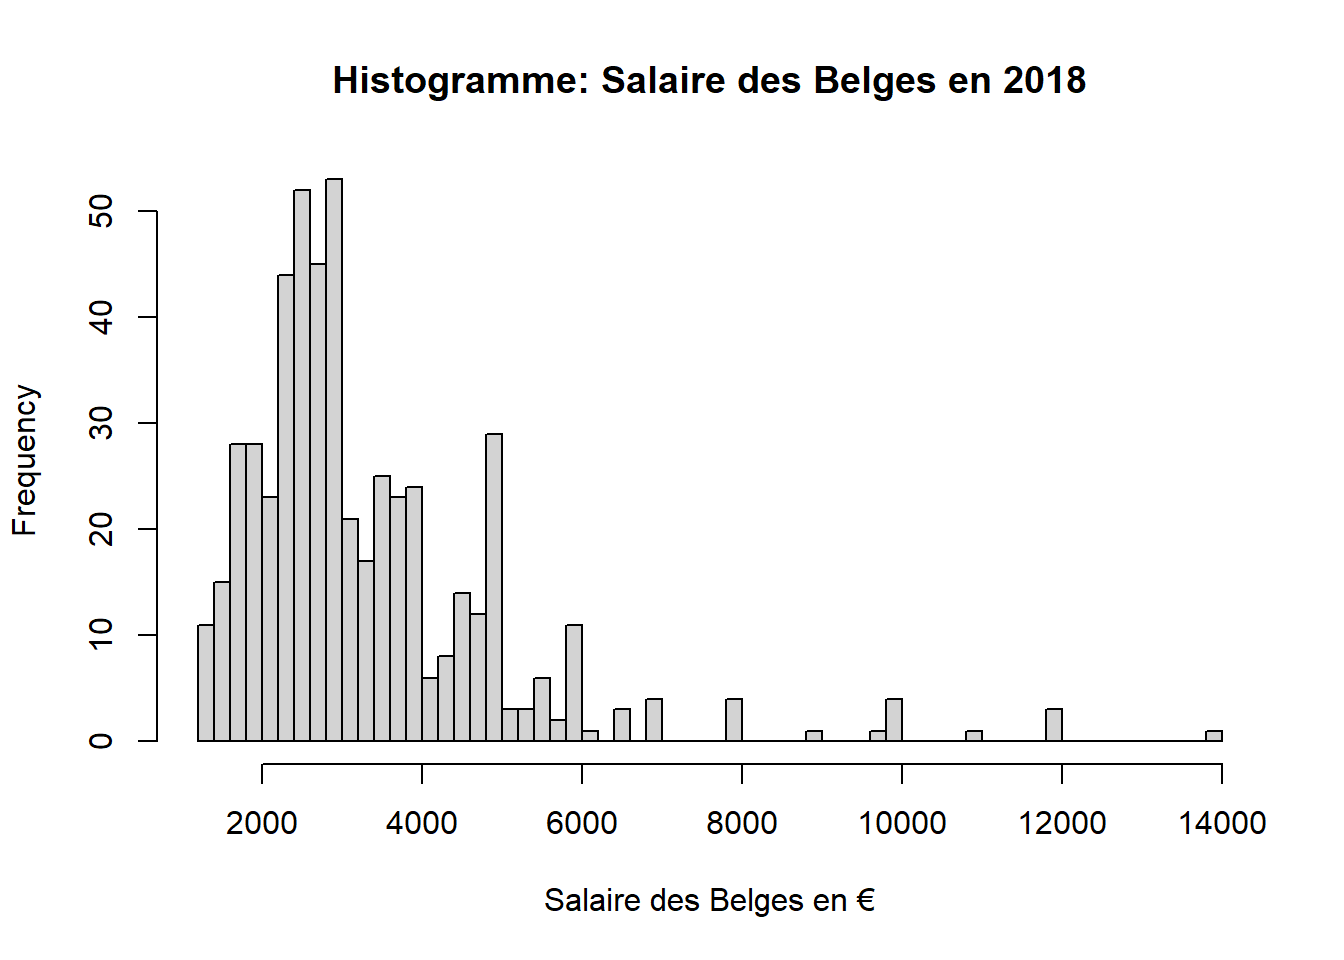
\includegraphics{bookdown-demo_files/figure-latex/unnamed-chunk-68-1.pdf}

Grâce à ce graphique l'on voit visuellement où se situent les \(10\%\) de probabilité de percevoir entre \(2500€\) et \(2800€\).

  \bibliography{book.bib,packages.bib}

\end{document}
